\clearpage
\begin{apendicesenv}
\partapendices

\chapter{Frontend Gallery}
\label{app:frontend}

This appendix brings together high-resolution captures of the \textit{G-FShield} operational interface. The purpose is to show navigation, analytical panels, and administrative screens without polluting the dissertation's main flow.
The images are organized by usage function so that the reader can clearly follow the progression from authentication to comparison, monitoring, and administration.

\section{Access and Overview}

The first screens present the platform entry point and the initial dashboard, and Figures~\ref{fig:app-front-sign-in} and~\ref{fig:app-front-overview} show that transition from access to consolidated overview.

\begin{figure}[!htb]
  \centering
  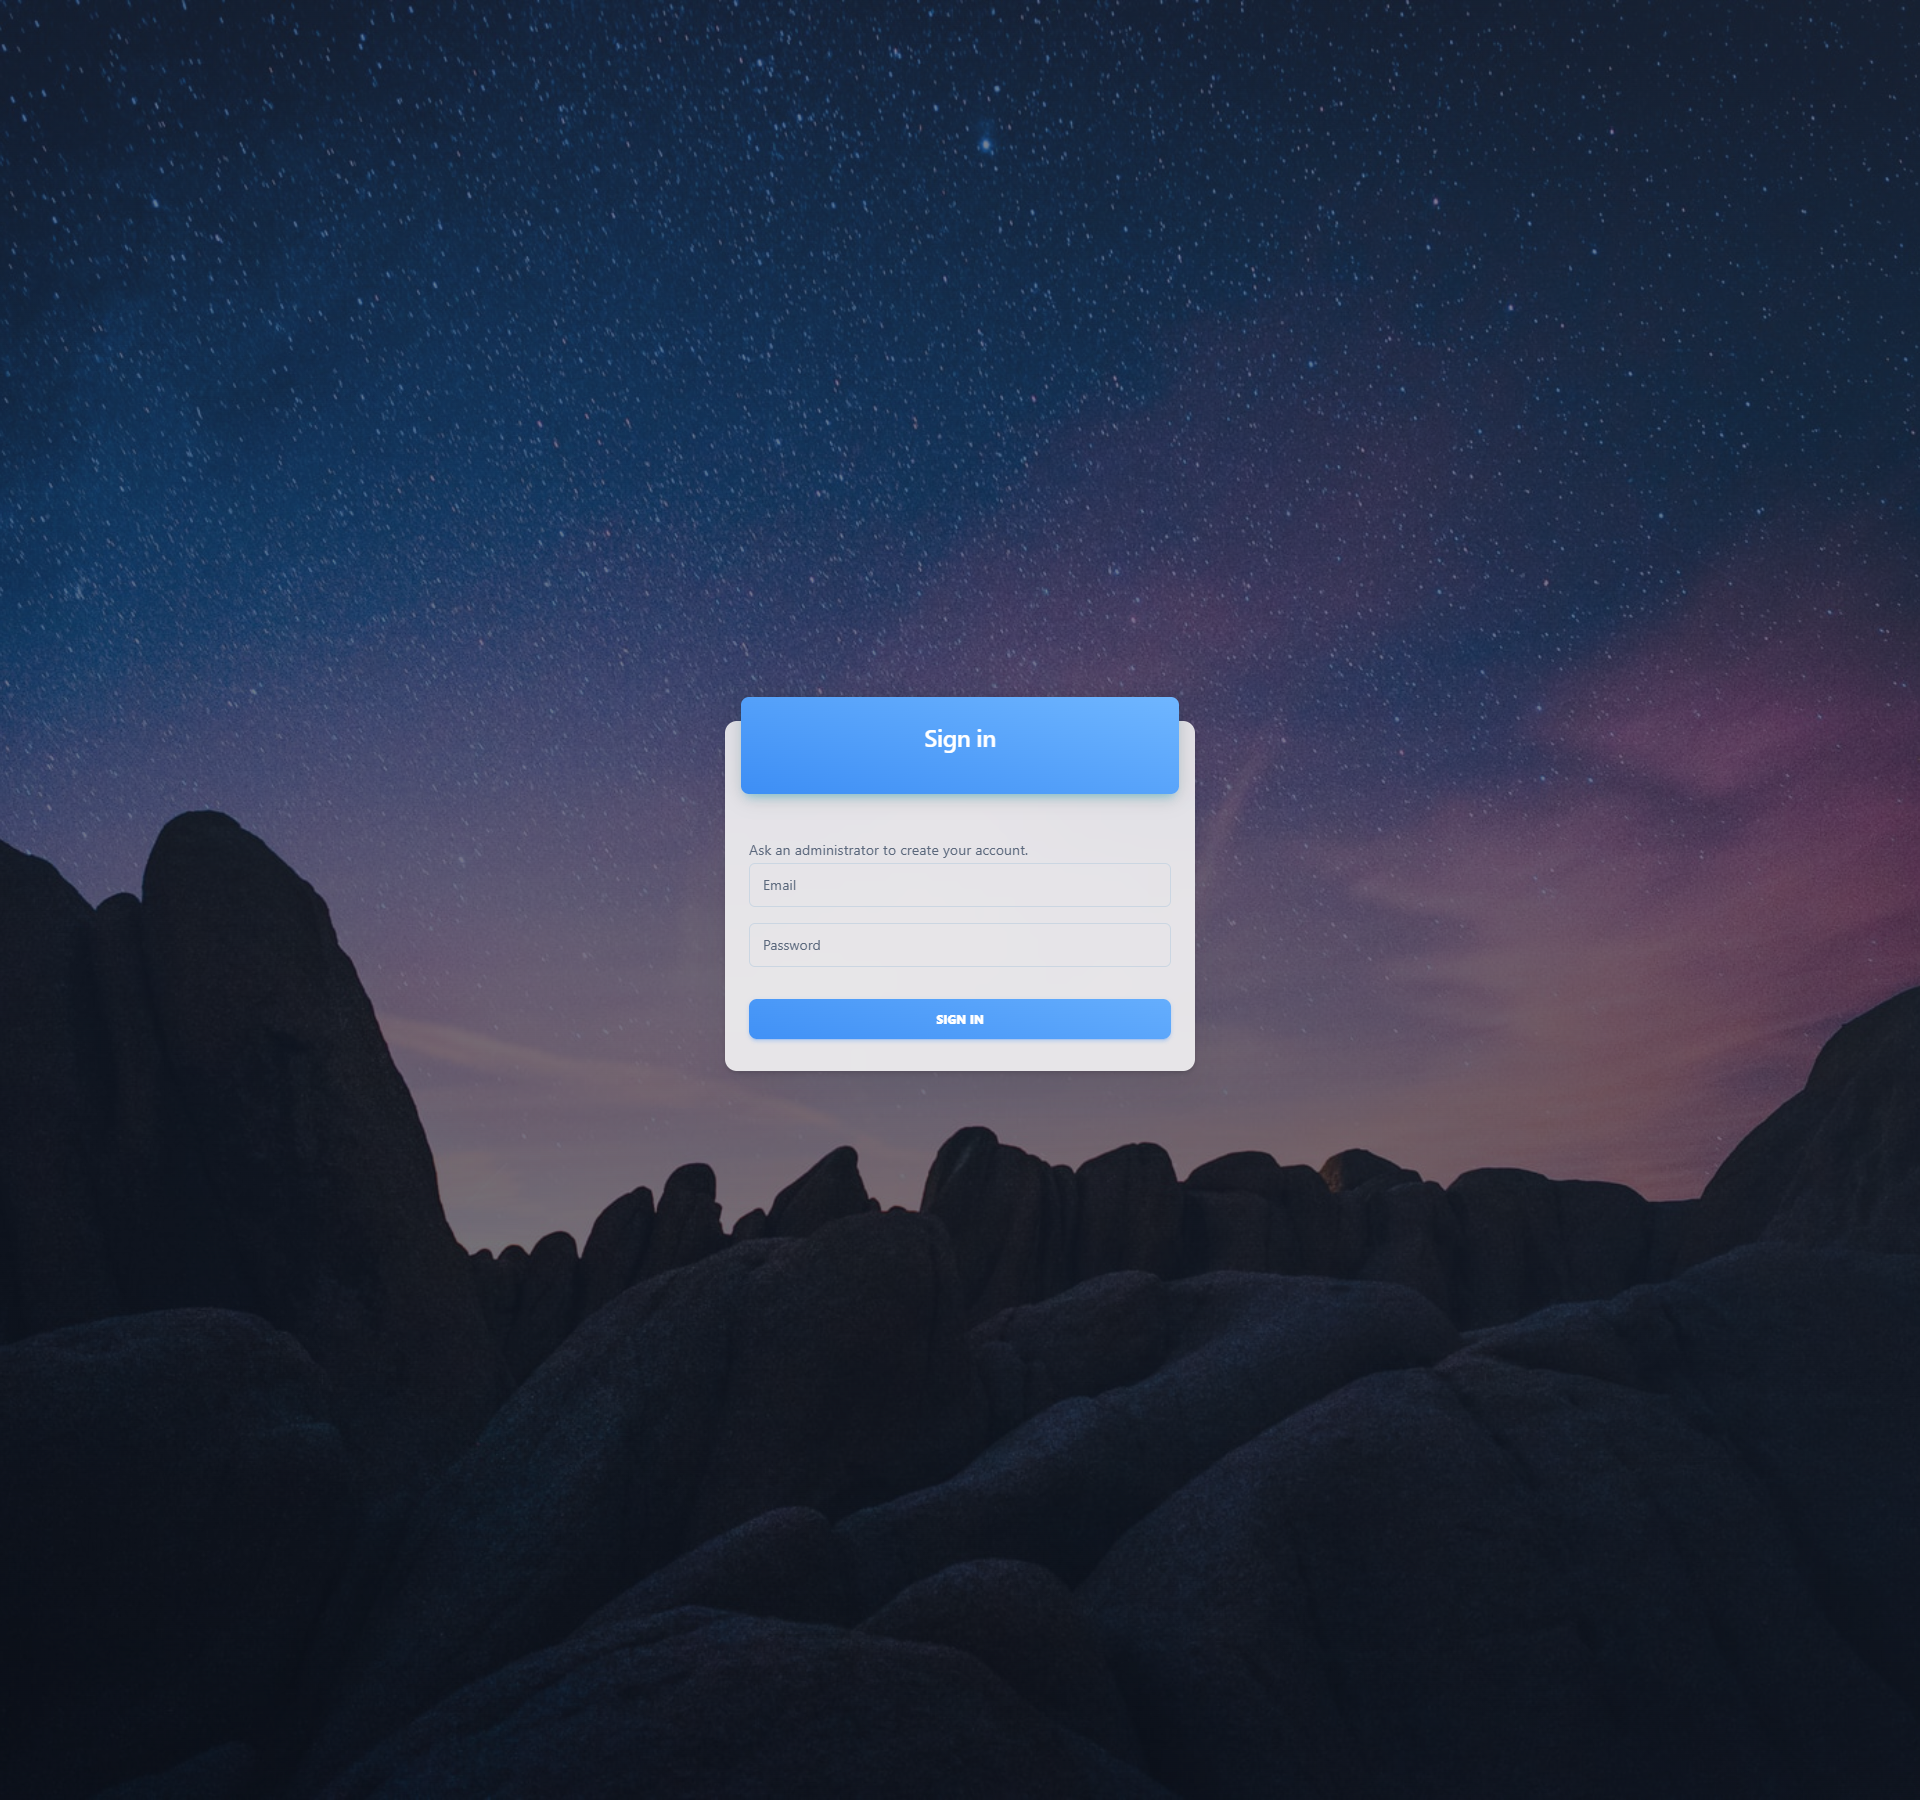
\includegraphics[width=\linewidth,height=0.80\textheight,keepaspectratio]{fig/front/00-sign-in.png}
  \caption{Authentication screen.}
  \label{fig:app-front-sign-in}
\end{figure}

\begin{figure}[!htb]
  \centering
  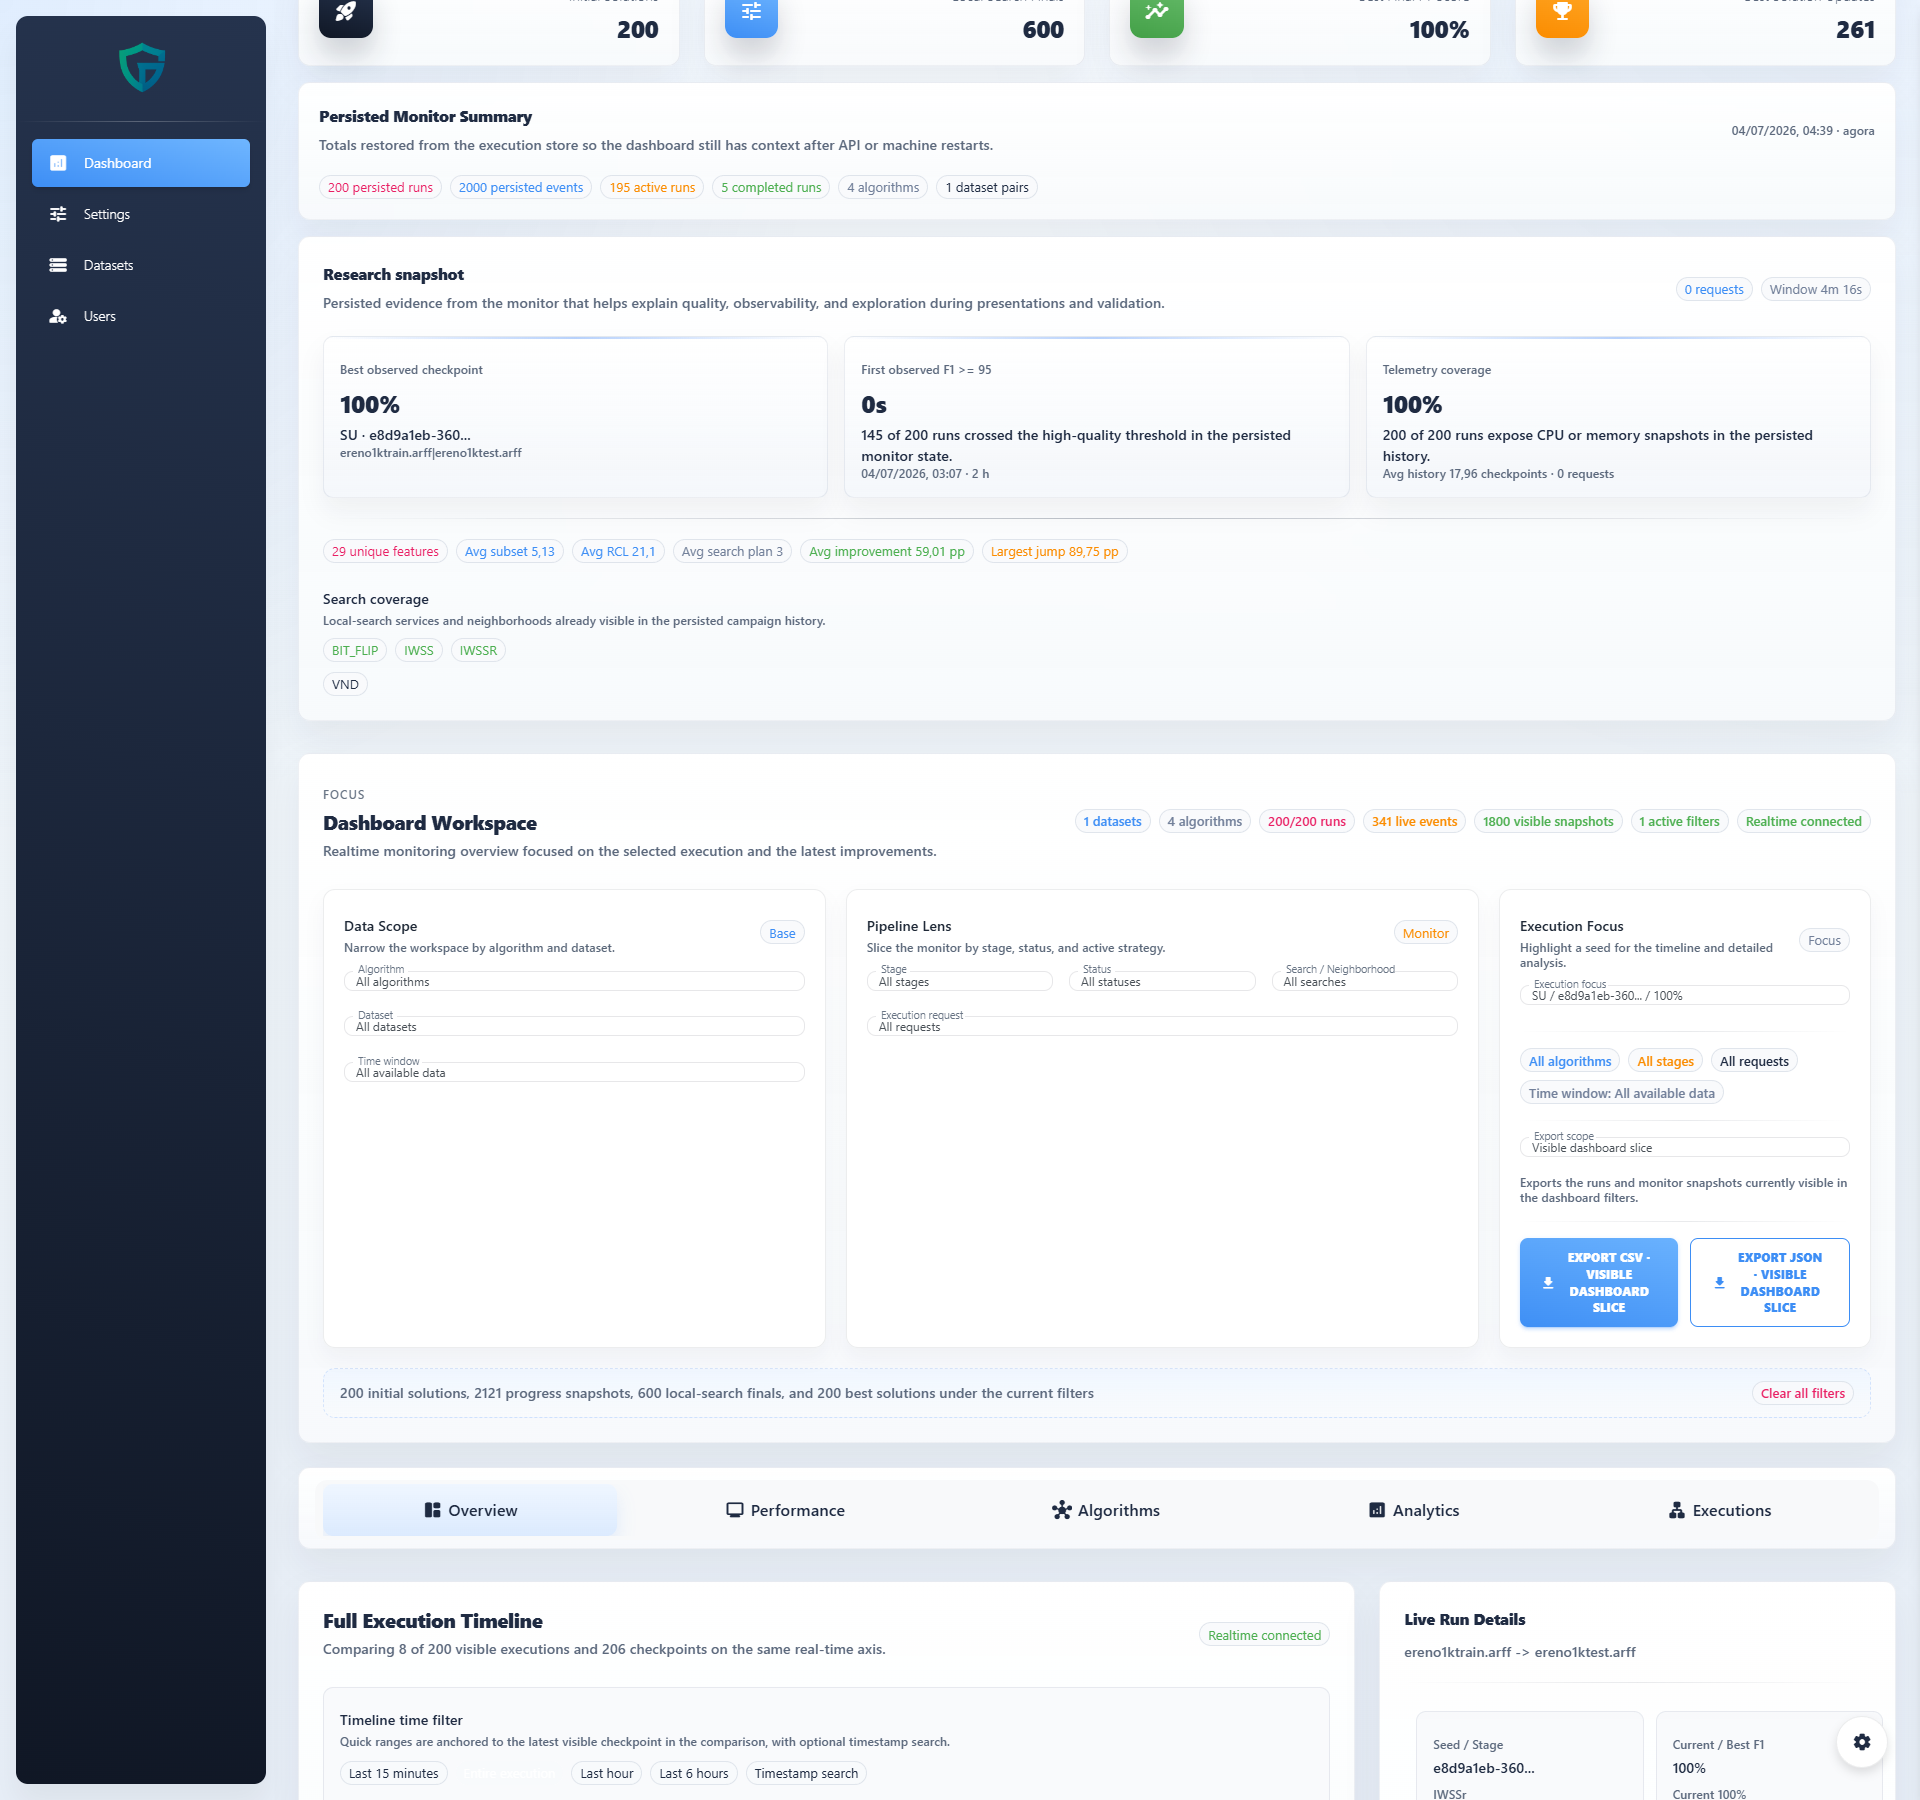
\includegraphics[width=\linewidth,height=0.80\textheight,keepaspectratio]{fig/front/01-dashboard-overview.png}
  \caption{Overview dashboard.}
  \label{fig:app-front-overview}
\end{figure}

\clearpage
\section{Performance and Algorithms}

This section shows how the user moves between the performance and algorithm-comparison panels, and Figures~\ref{fig:app-front-performance} and~\ref{fig:app-front-algorithms} detail that reading.

\begin{figure}[!htb]
  \centering
  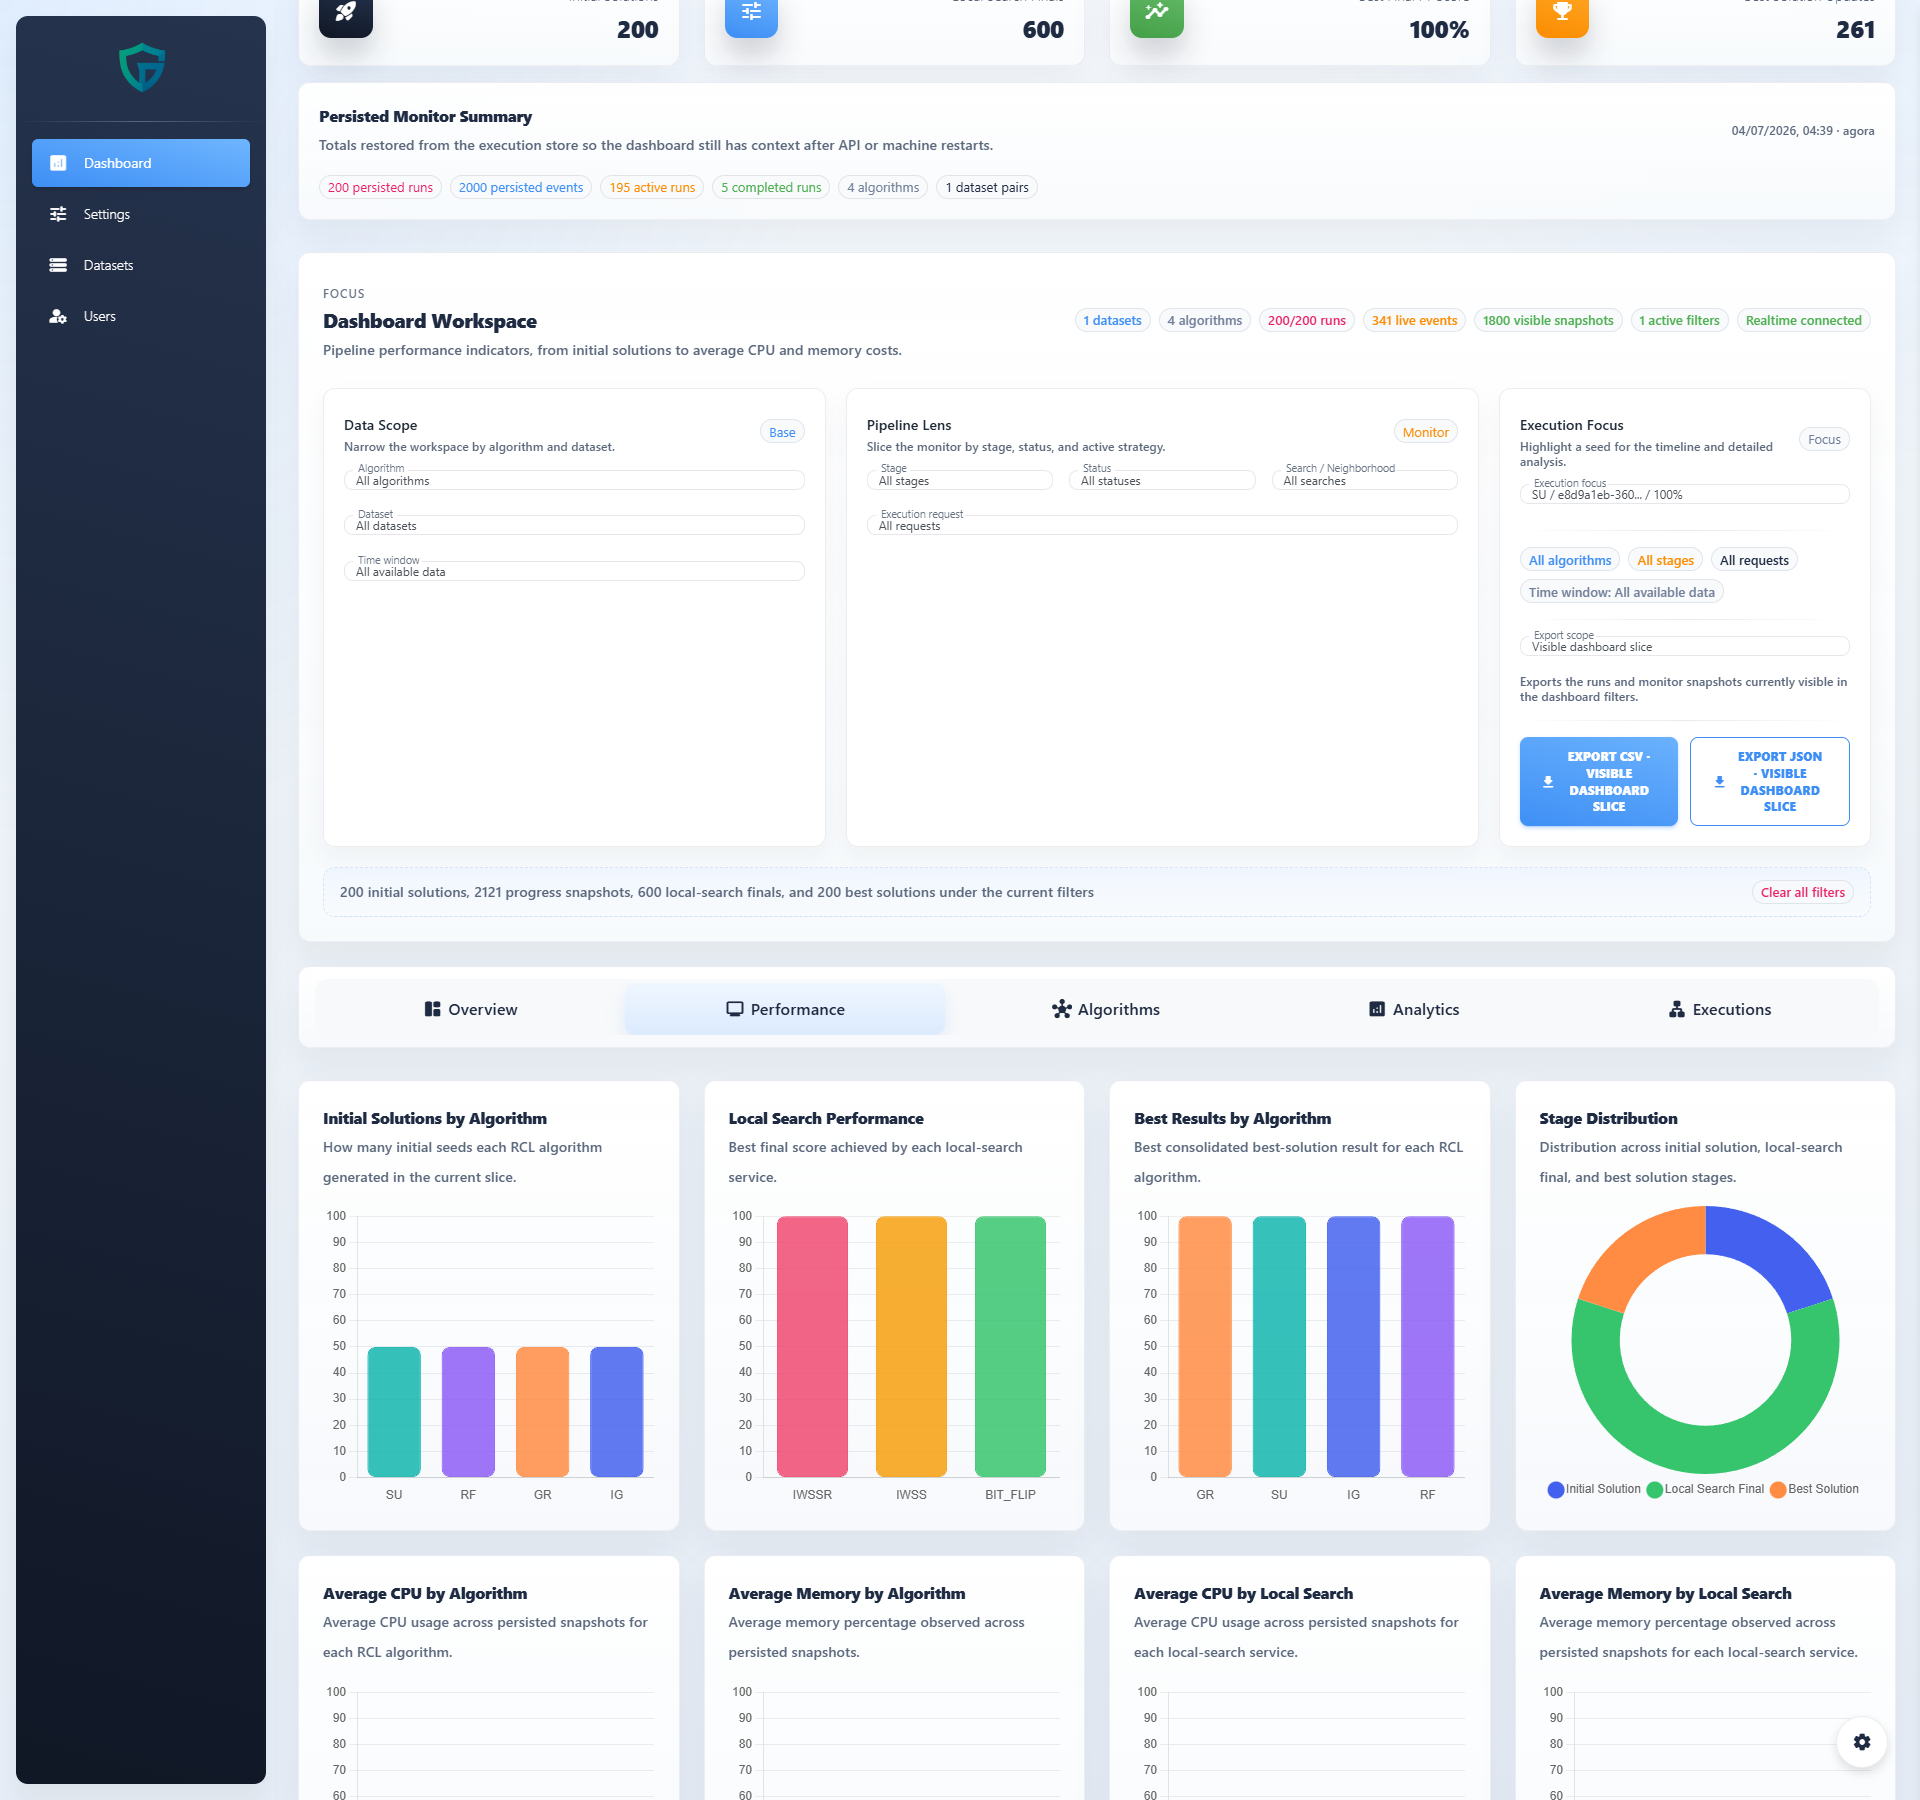
\includegraphics[width=\linewidth,height=0.80\textheight,keepaspectratio]{fig/front/02-dashboard-performance.png}
  \caption{Performance screen.}
  \label{fig:app-front-performance}
\end{figure}

\begin{figure}[!htb]
  \centering
  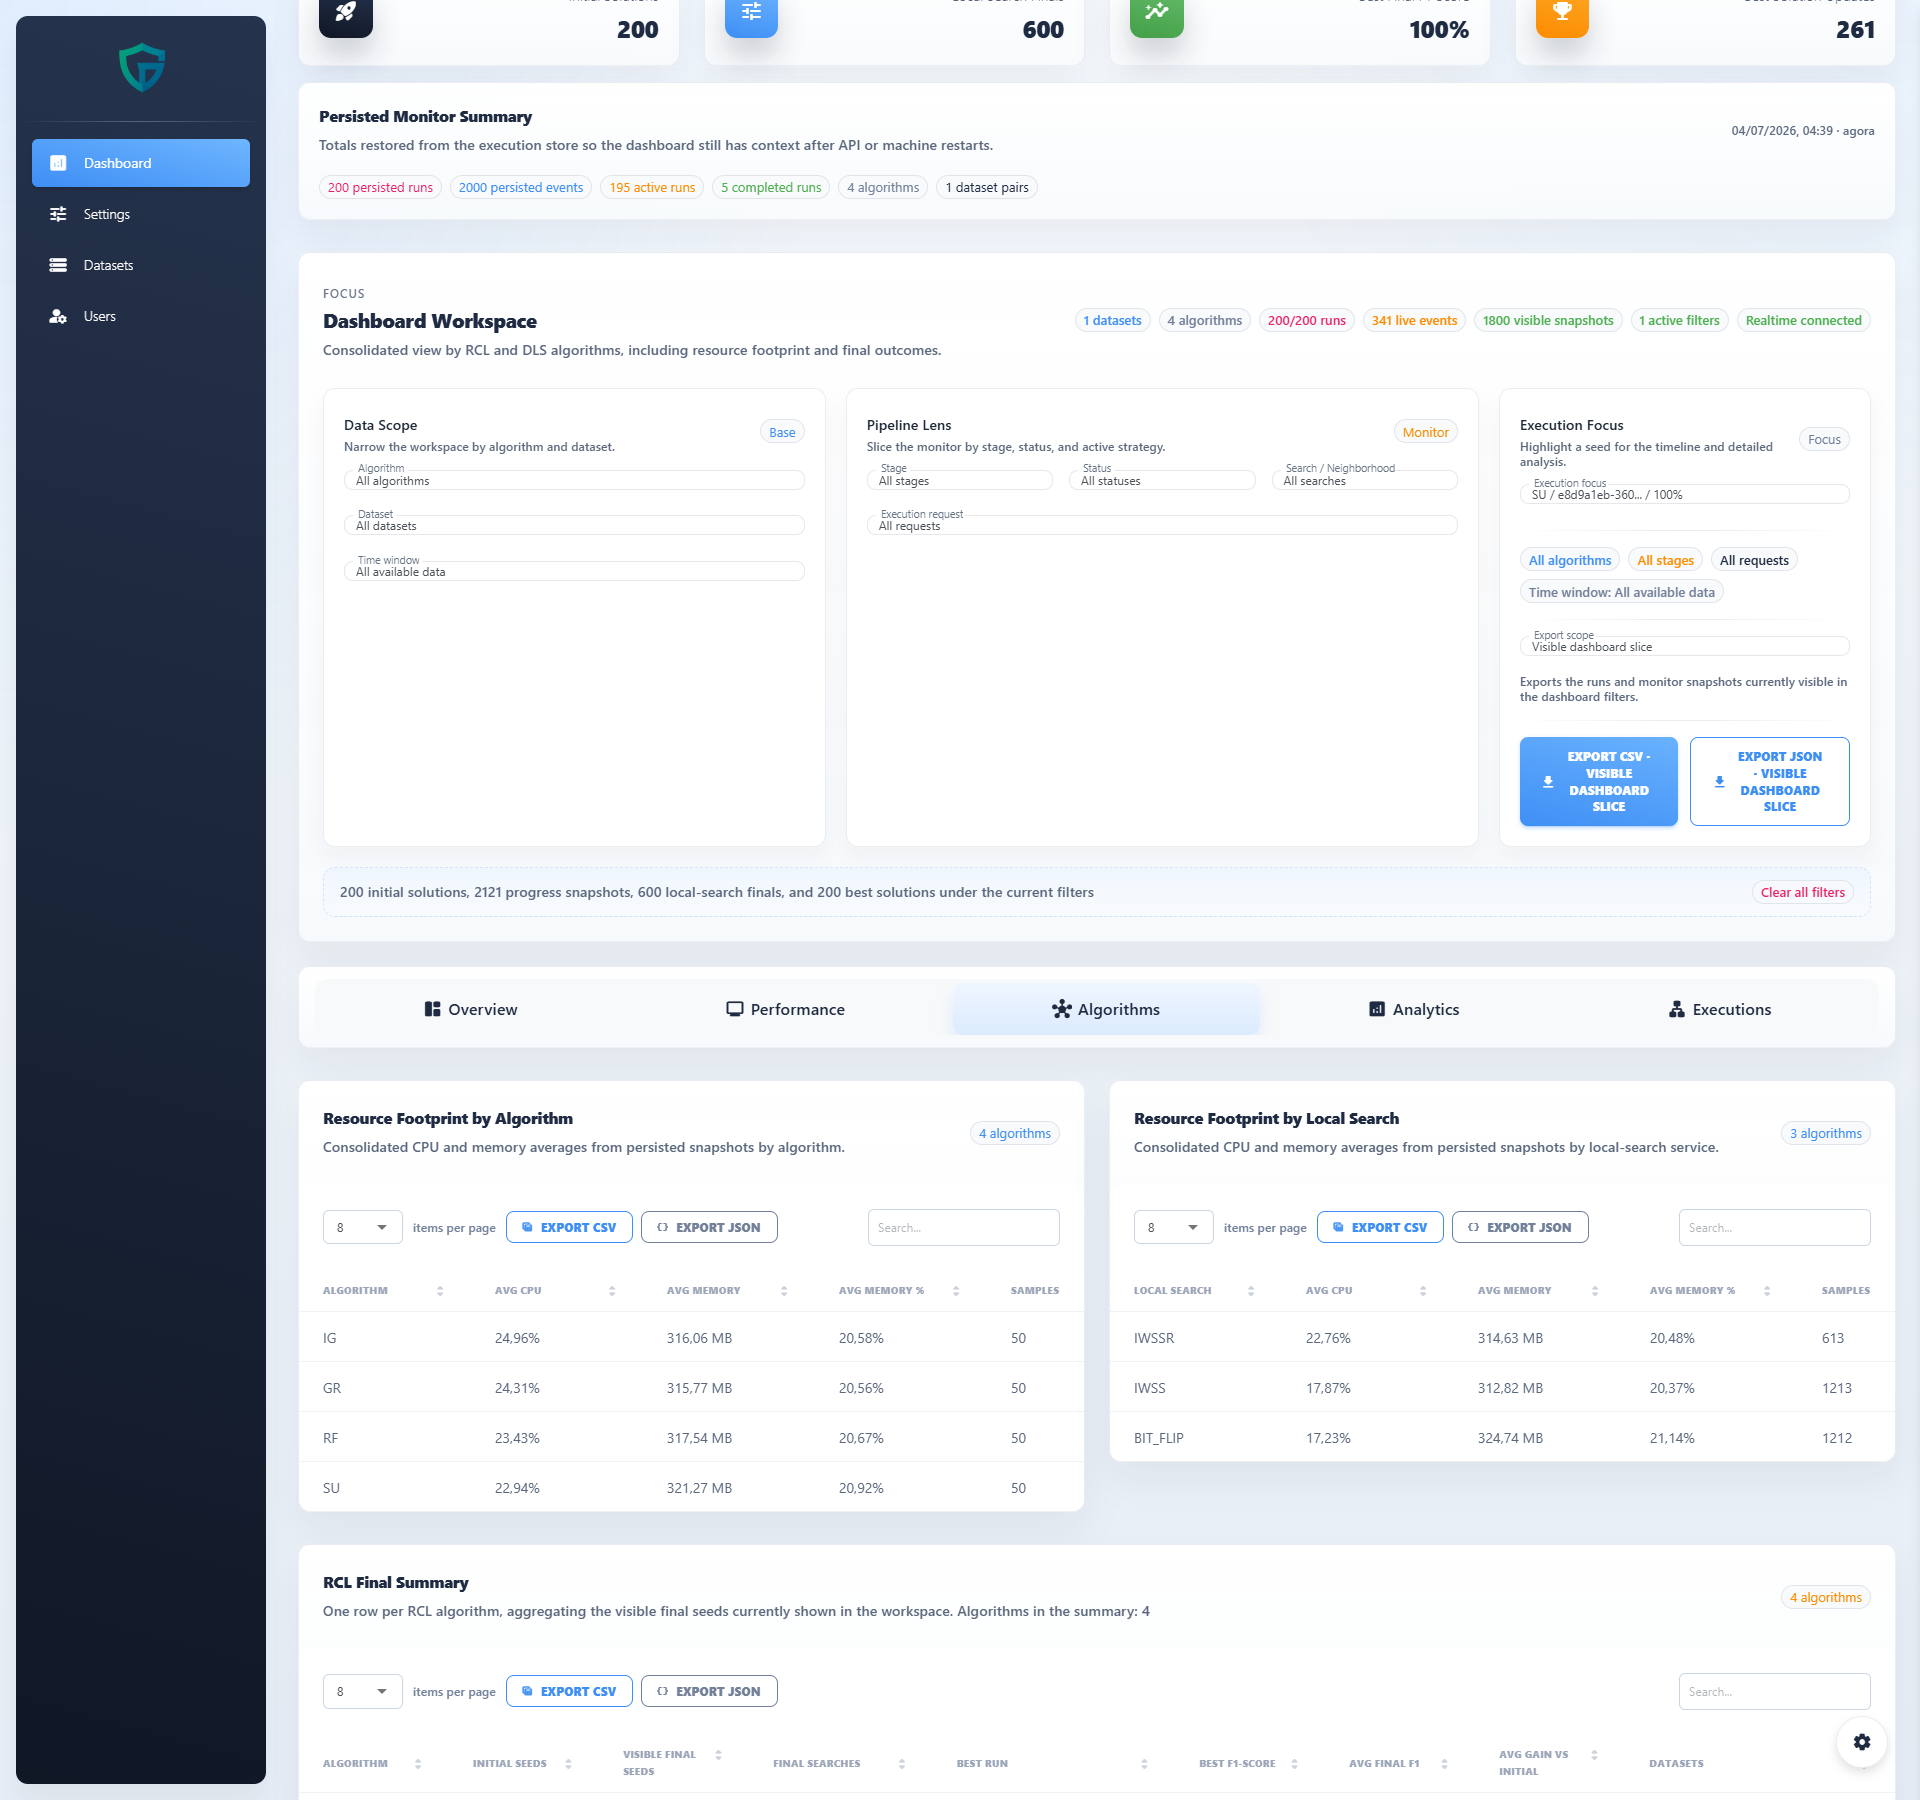
\includegraphics[width=\linewidth,height=0.80\textheight,keepaspectratio]{fig/front/03-dashboard-algorithms.png}
  \caption{Algorithm comparison screen.}
  \label{fig:app-front-algorithms}
\end{figure}

\clearpage
\section{Analytics}

The analytics panels summarize execution activity and help expose aggregate trends, event-level details, and persisted topics.
Figures~\ref{fig:app-front-analytics-activity},~\ref{fig:app-front-analytics-activity-detail},~\ref{fig:app-front-analytics-topics}, and~\ref{fig:app-front-analytics-feed} organize that view in layers.

\begin{figure}[!htb]
  \centering
  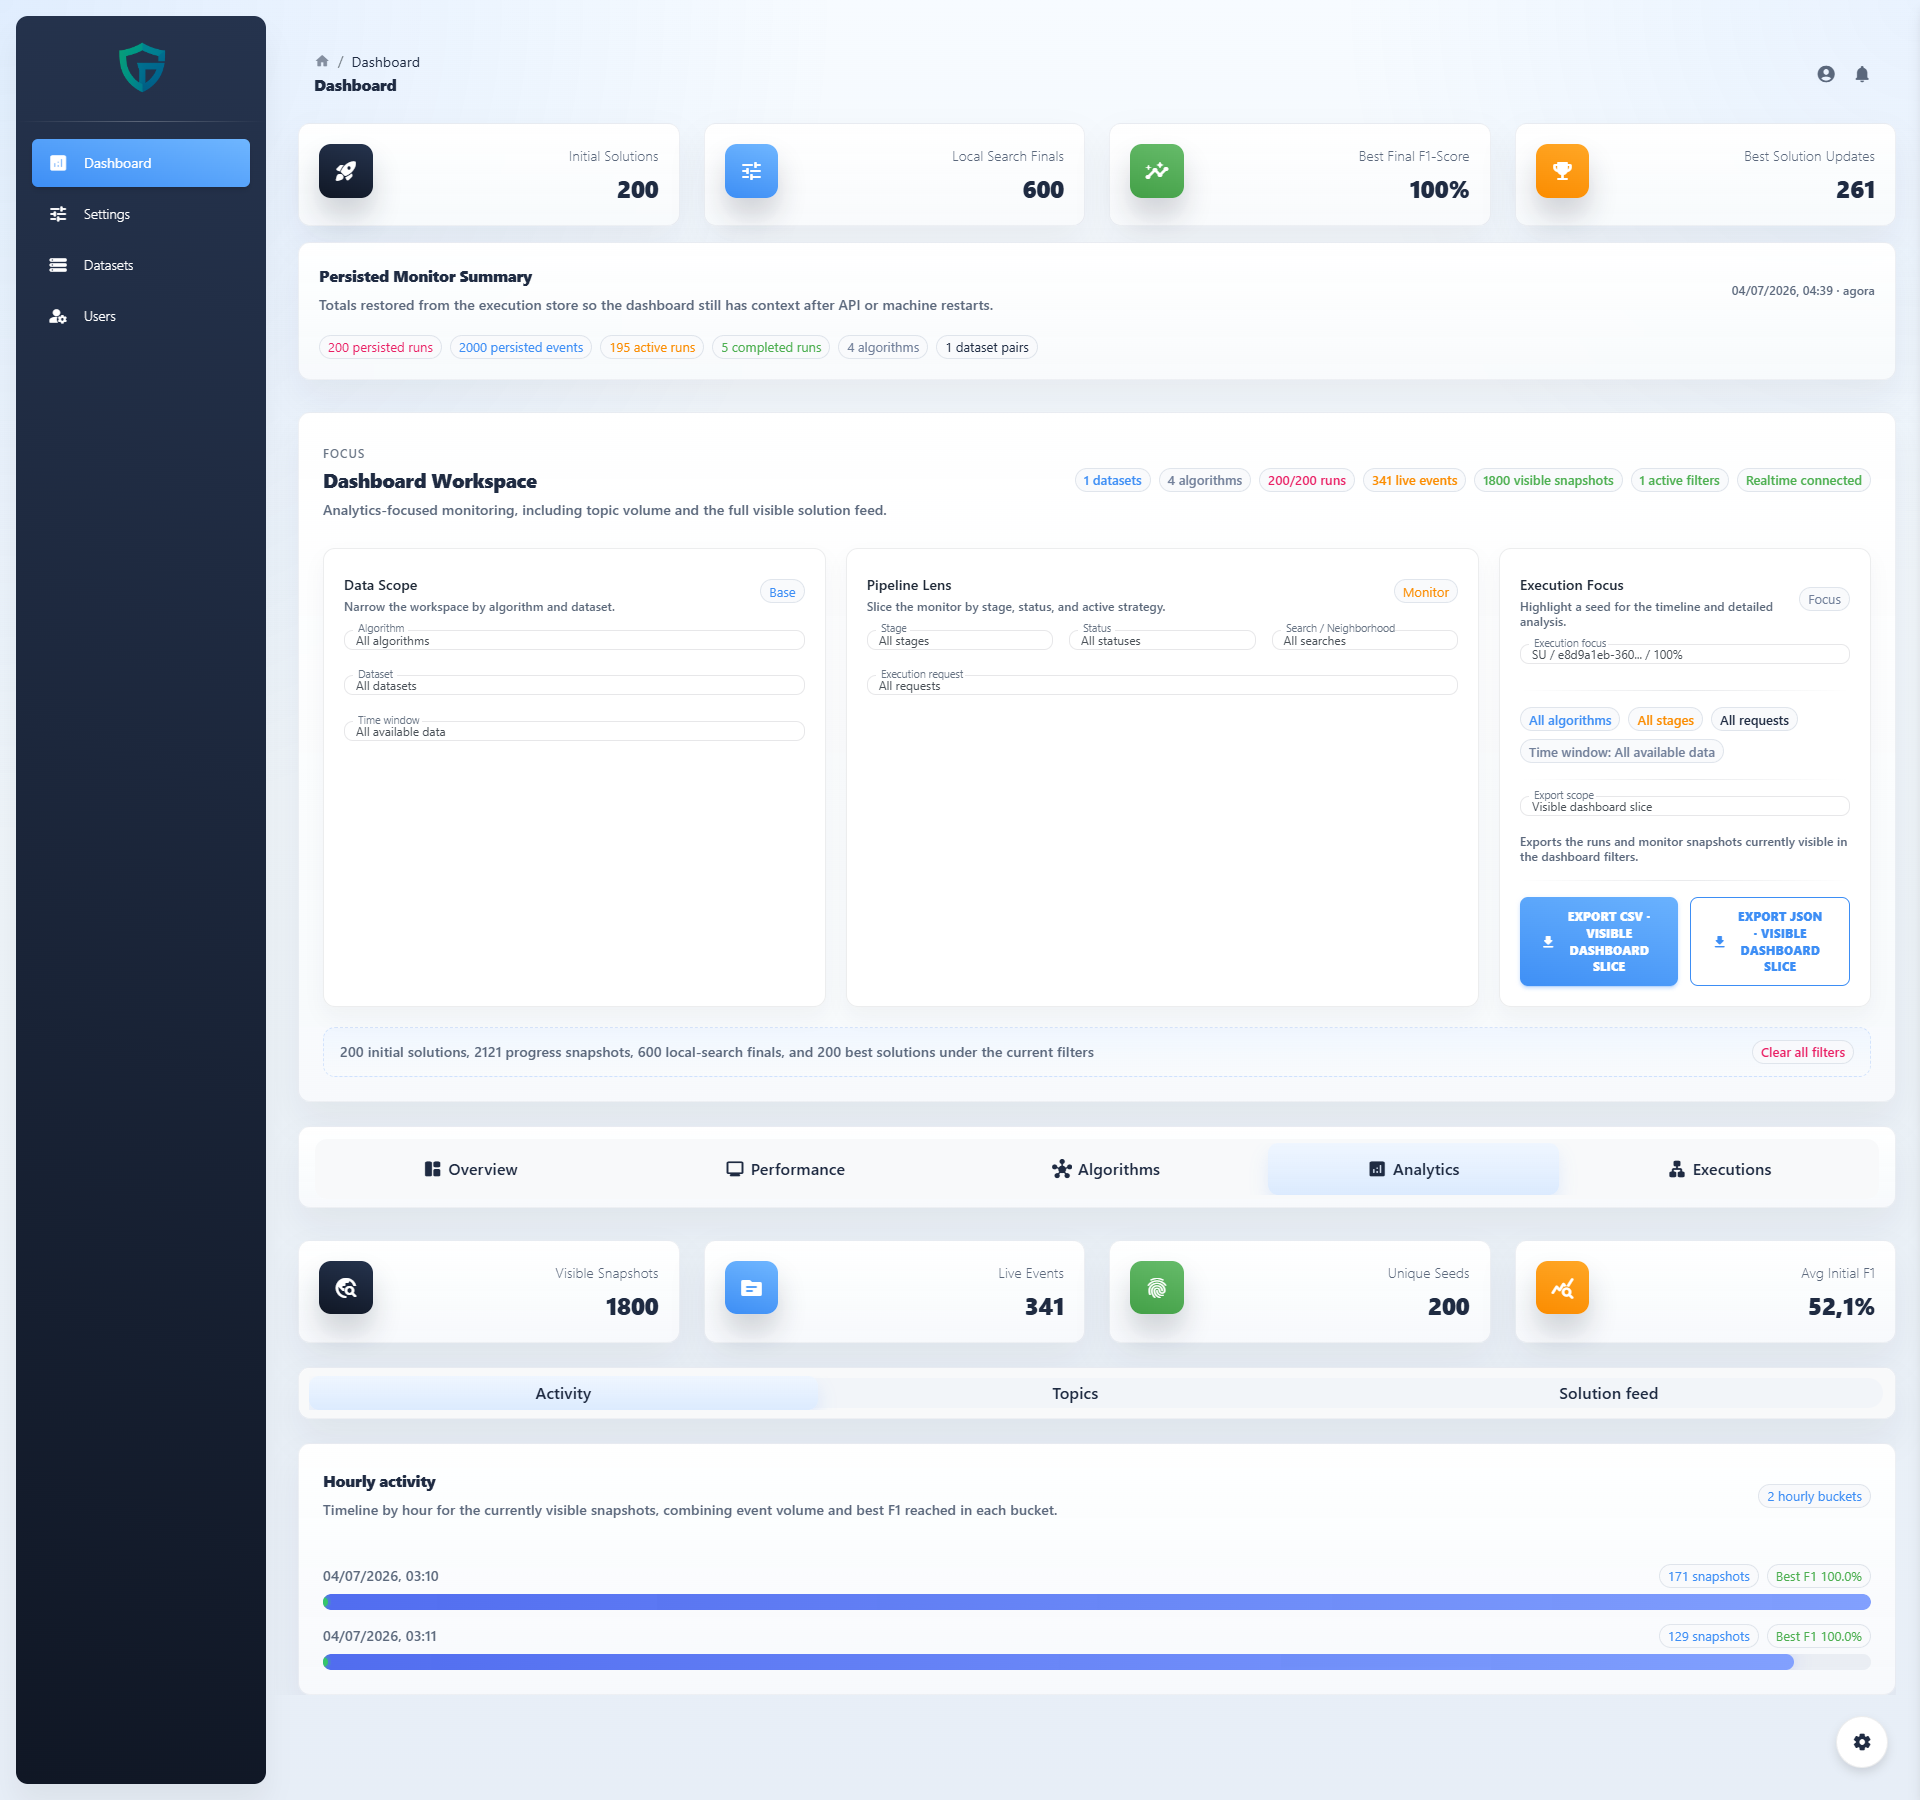
\includegraphics[width=\linewidth,height=0.80\textheight,keepaspectratio]{fig/front/04-dashboard-analytics-activity.png}
  \caption{Aggregated analytics activity.}
  \label{fig:app-front-analytics-activity}
\end{figure}

\begin{figure}[!htb]
  \centering
  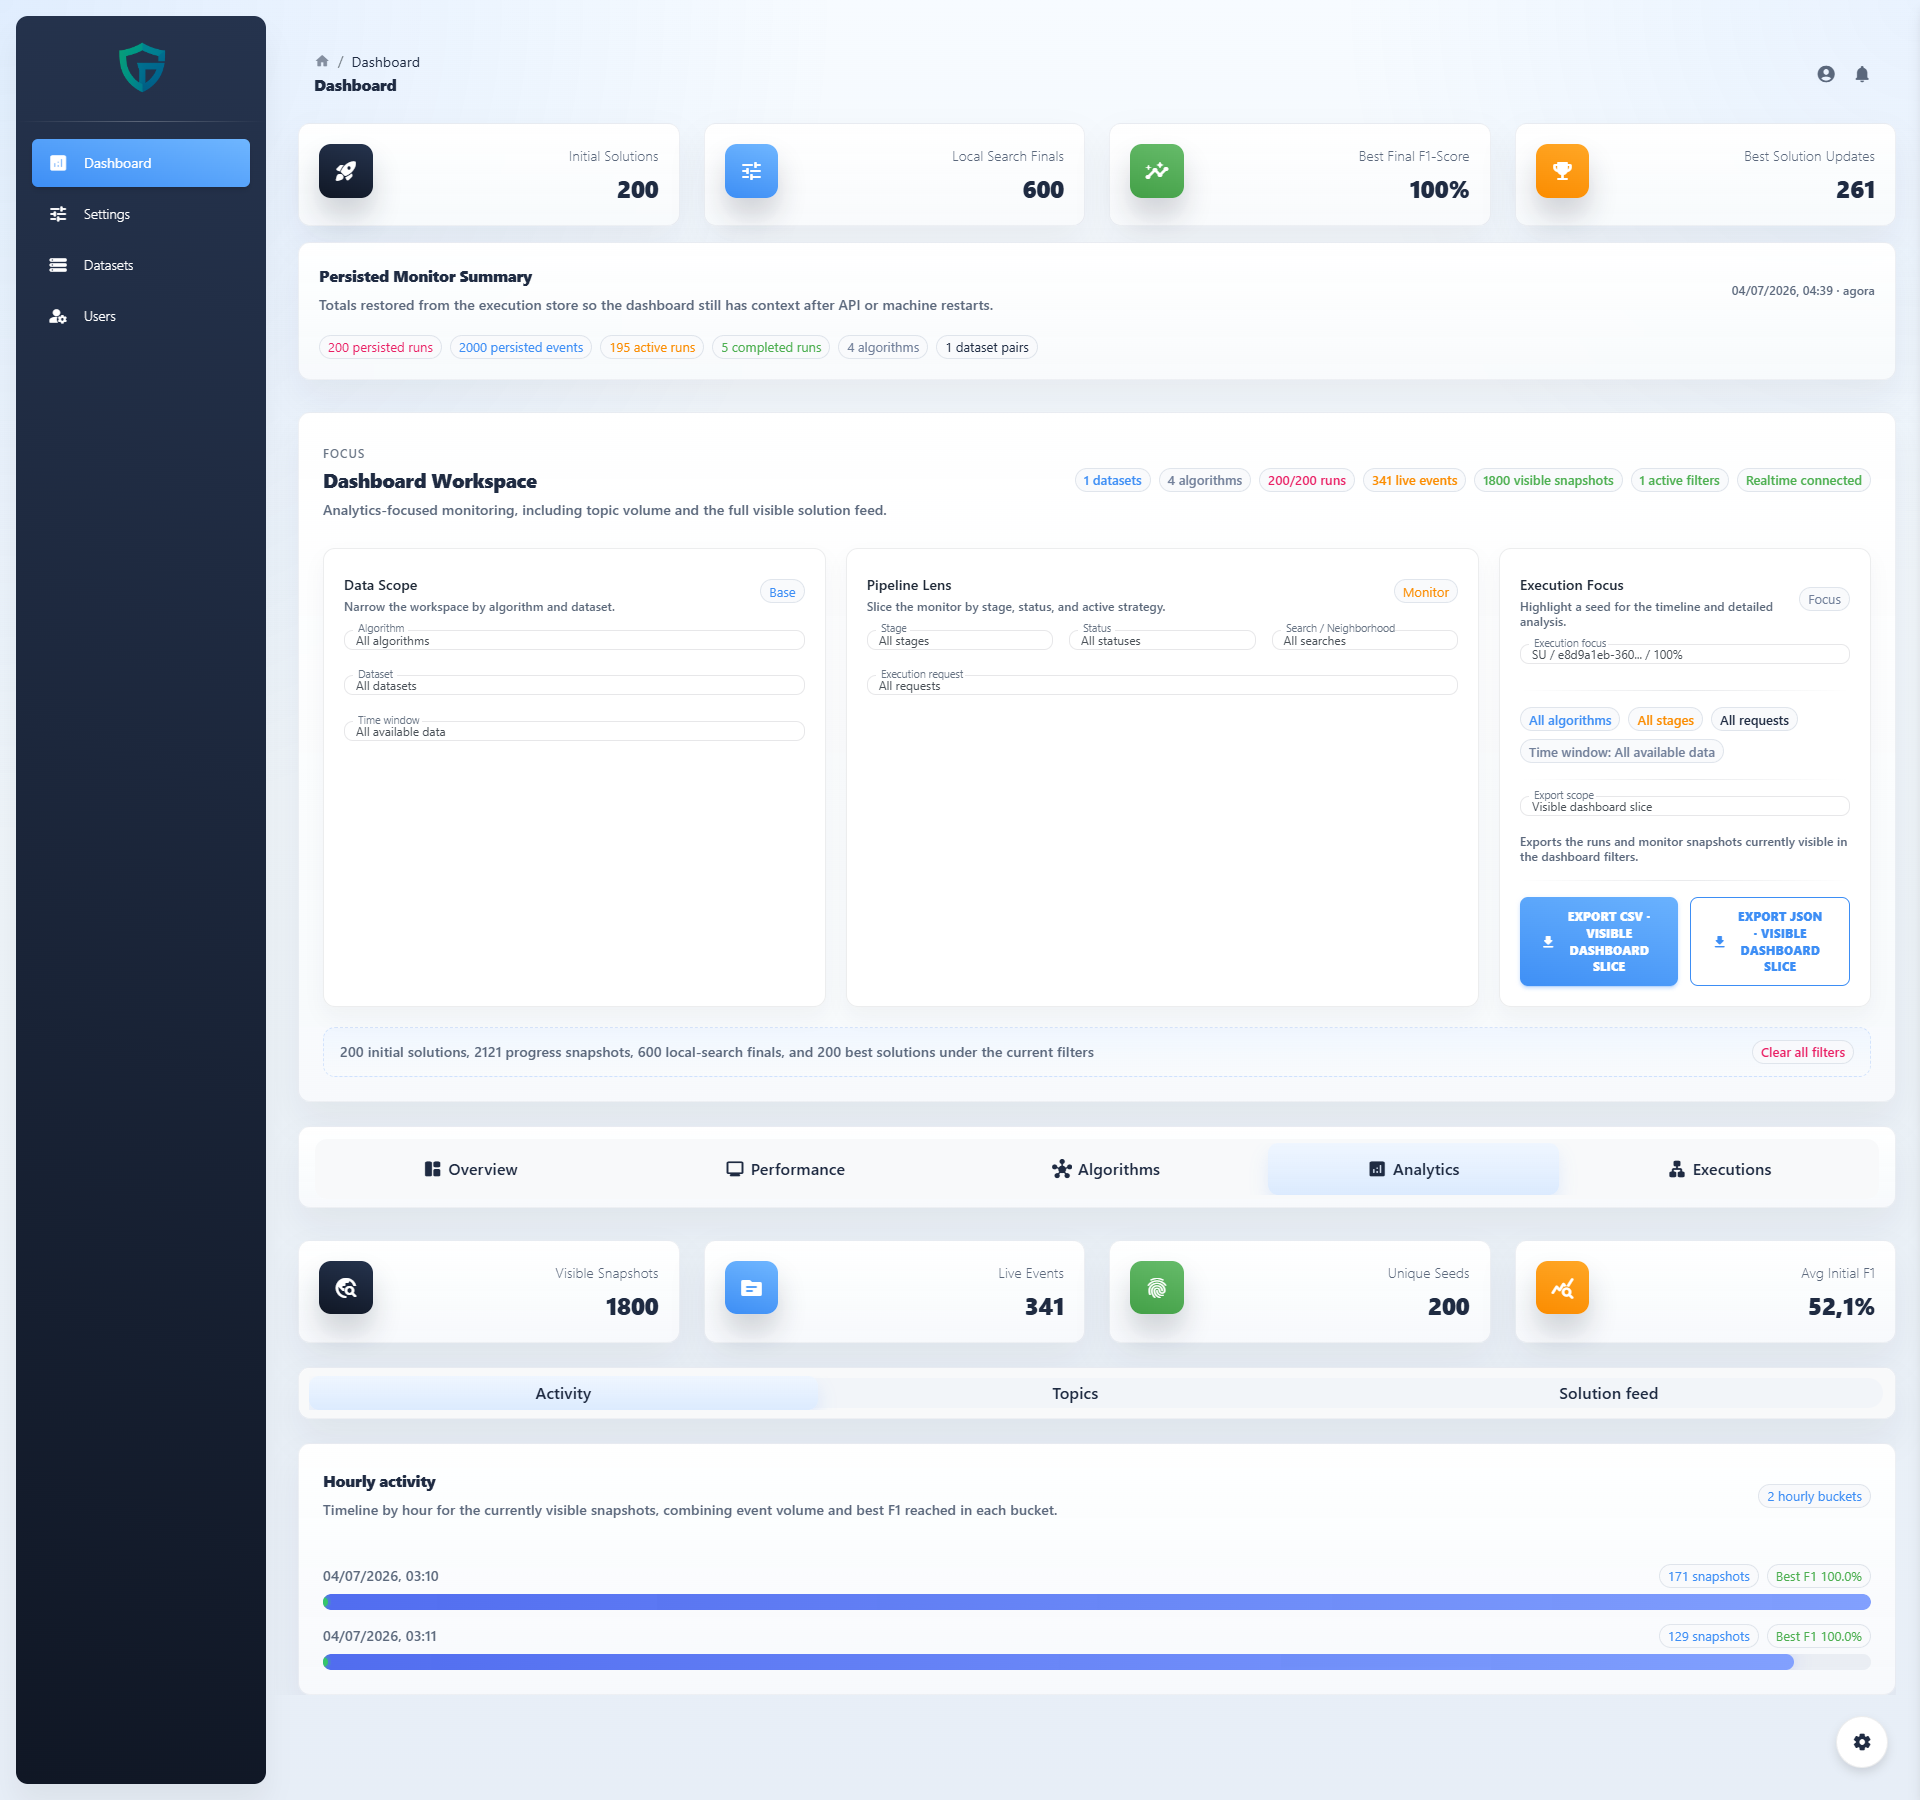
\includegraphics[width=\linewidth,height=0.80\textheight,keepaspectratio]{fig/front/05-dashboard-analytics-activity-detail.png}
  \caption{Analytics activity detail.}
  \label{fig:app-front-analytics-activity-detail}
\end{figure}

\begin{figure}[!htb]
  \centering
  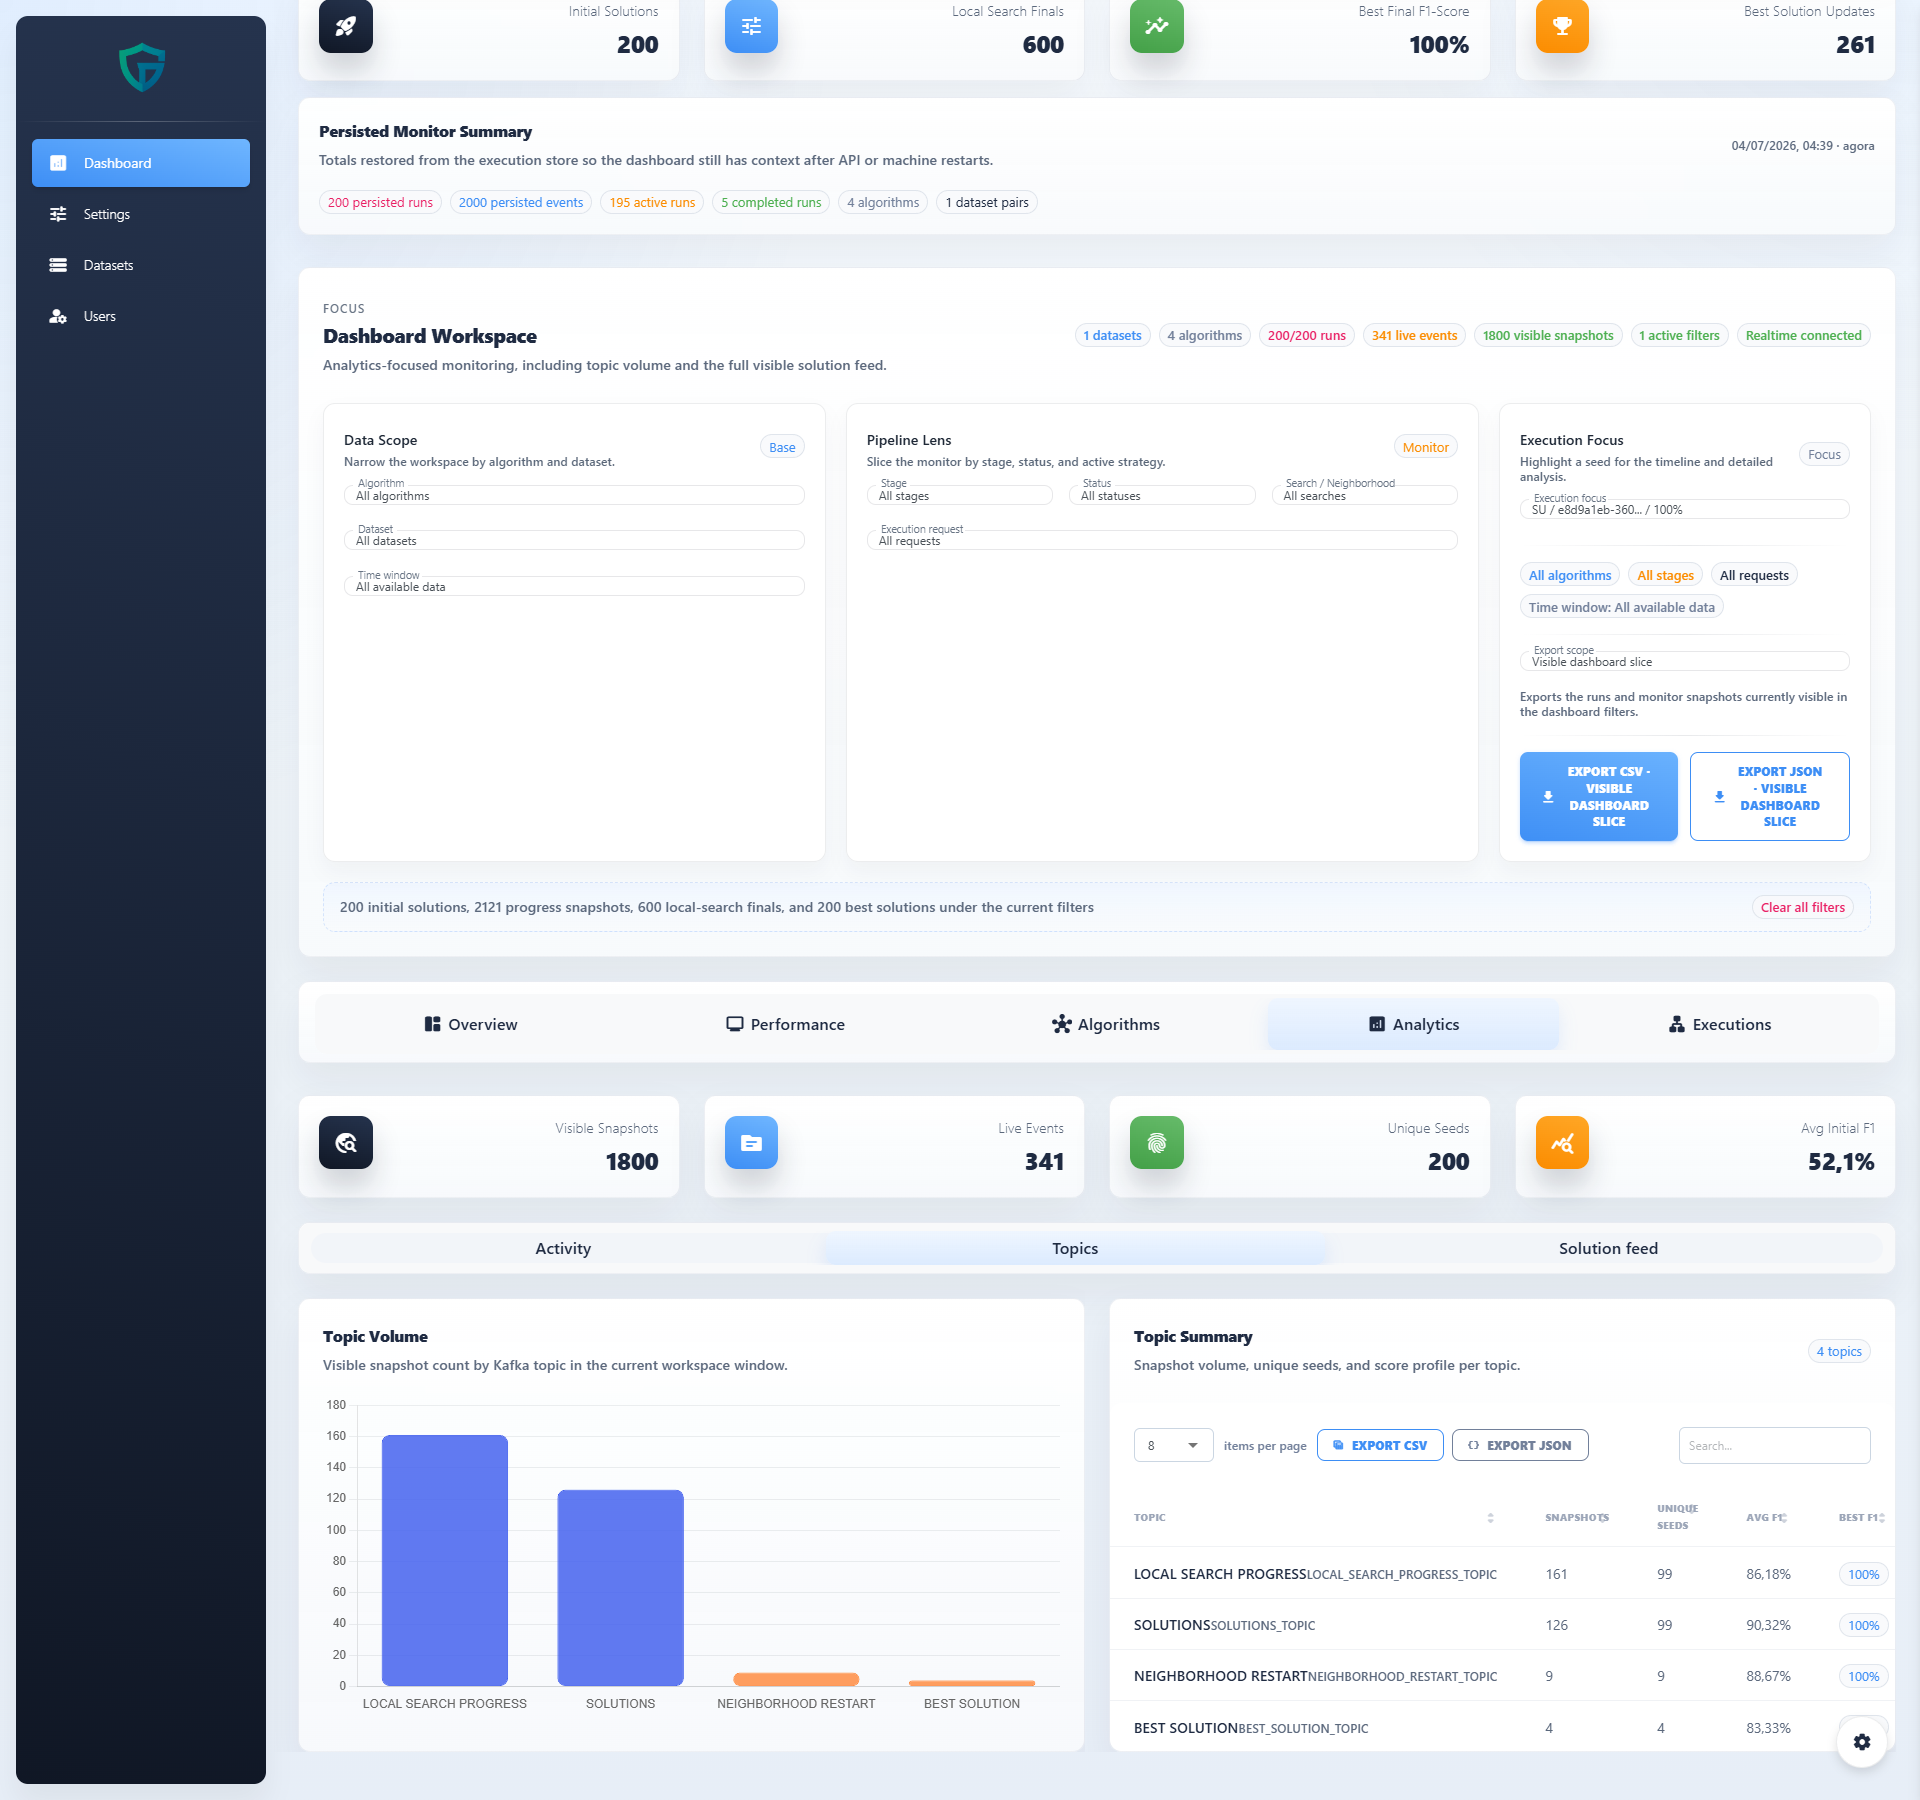
\includegraphics[width=\linewidth,height=0.80\textheight,keepaspectratio]{fig/front/06-dashboard-analytics-topics.png}
  \caption{Analytics topics.}
  \label{fig:app-front-analytics-topics}
\end{figure}

\begin{figure}[!htb]
  \centering
  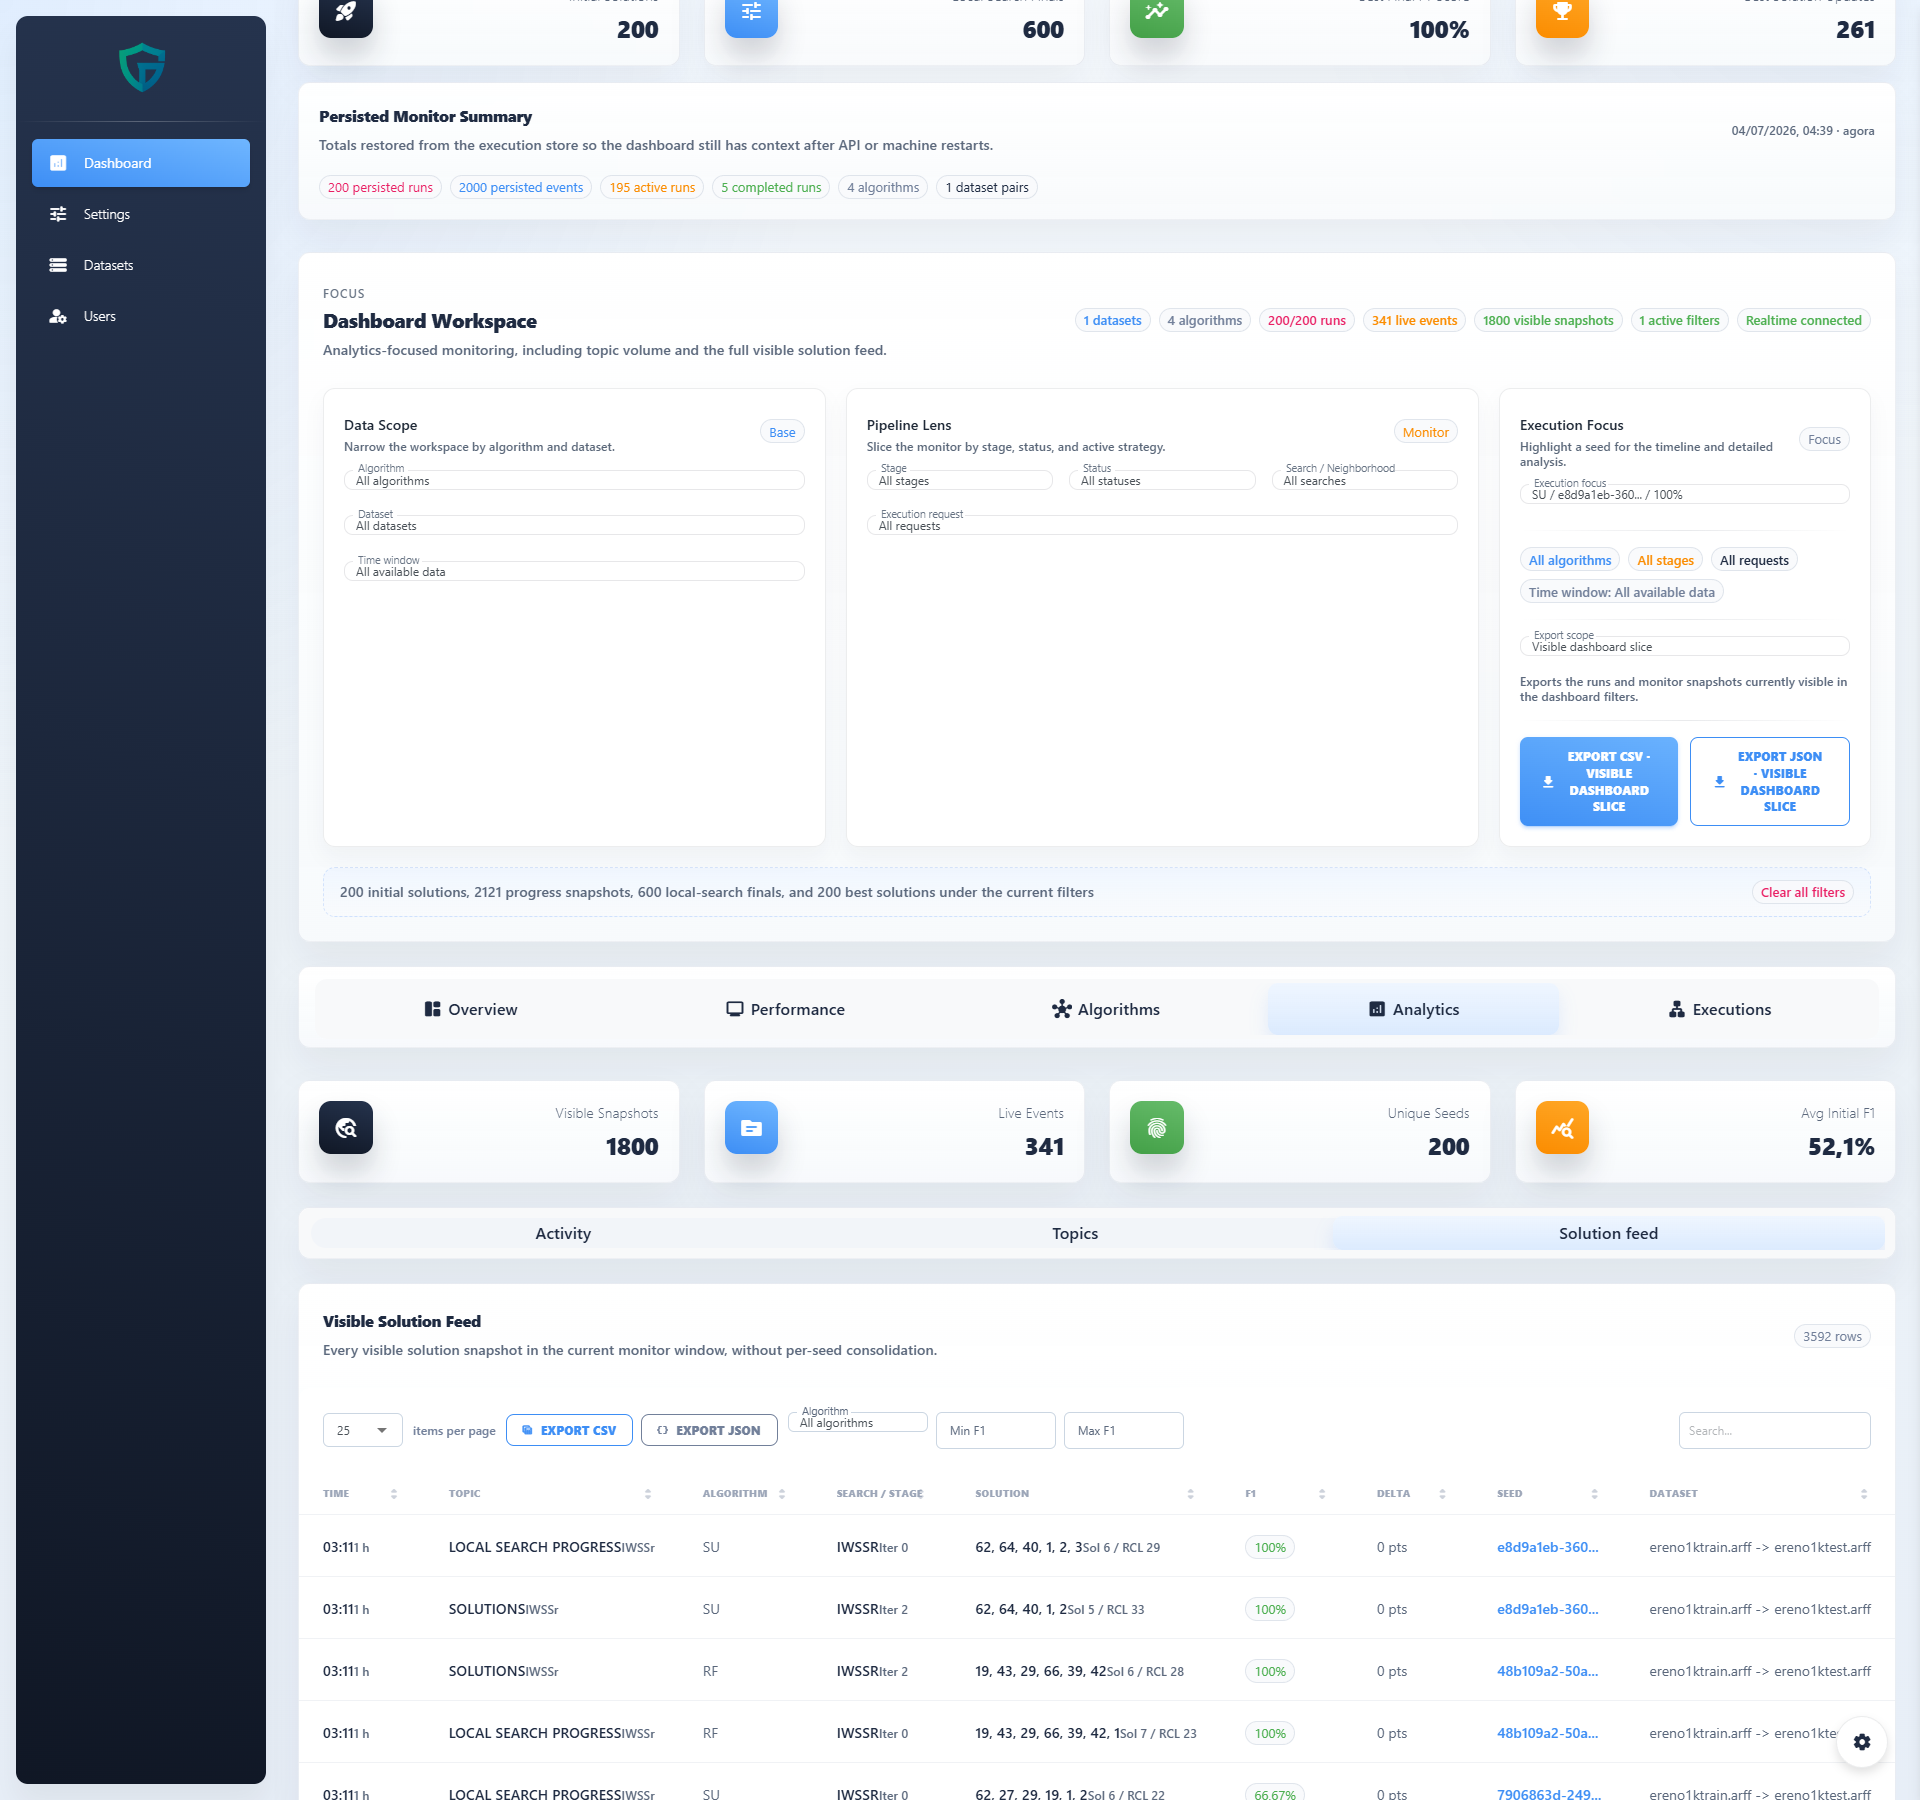
\includegraphics[width=\linewidth,height=0.80\textheight,keepaspectratio]{fig/front/07-dashboard-analytics-feed.png}
  \caption{Persisted analytics feed.}
  \label{fig:app-front-analytics-feed}
\end{figure}

\clearpage
\section{Run Comparison}

This part highlights run comparison and inspection of selected seeds, reinforcing the platform's exploratory and auditable nature.
Figures~\ref{fig:app-front-executions-comparison},~\ref{fig:app-front-executions-comparison-selected}, and~\ref{fig:app-front-run-details} show how that comparison works in practice.

\begin{figure}[!htb]
  \centering
  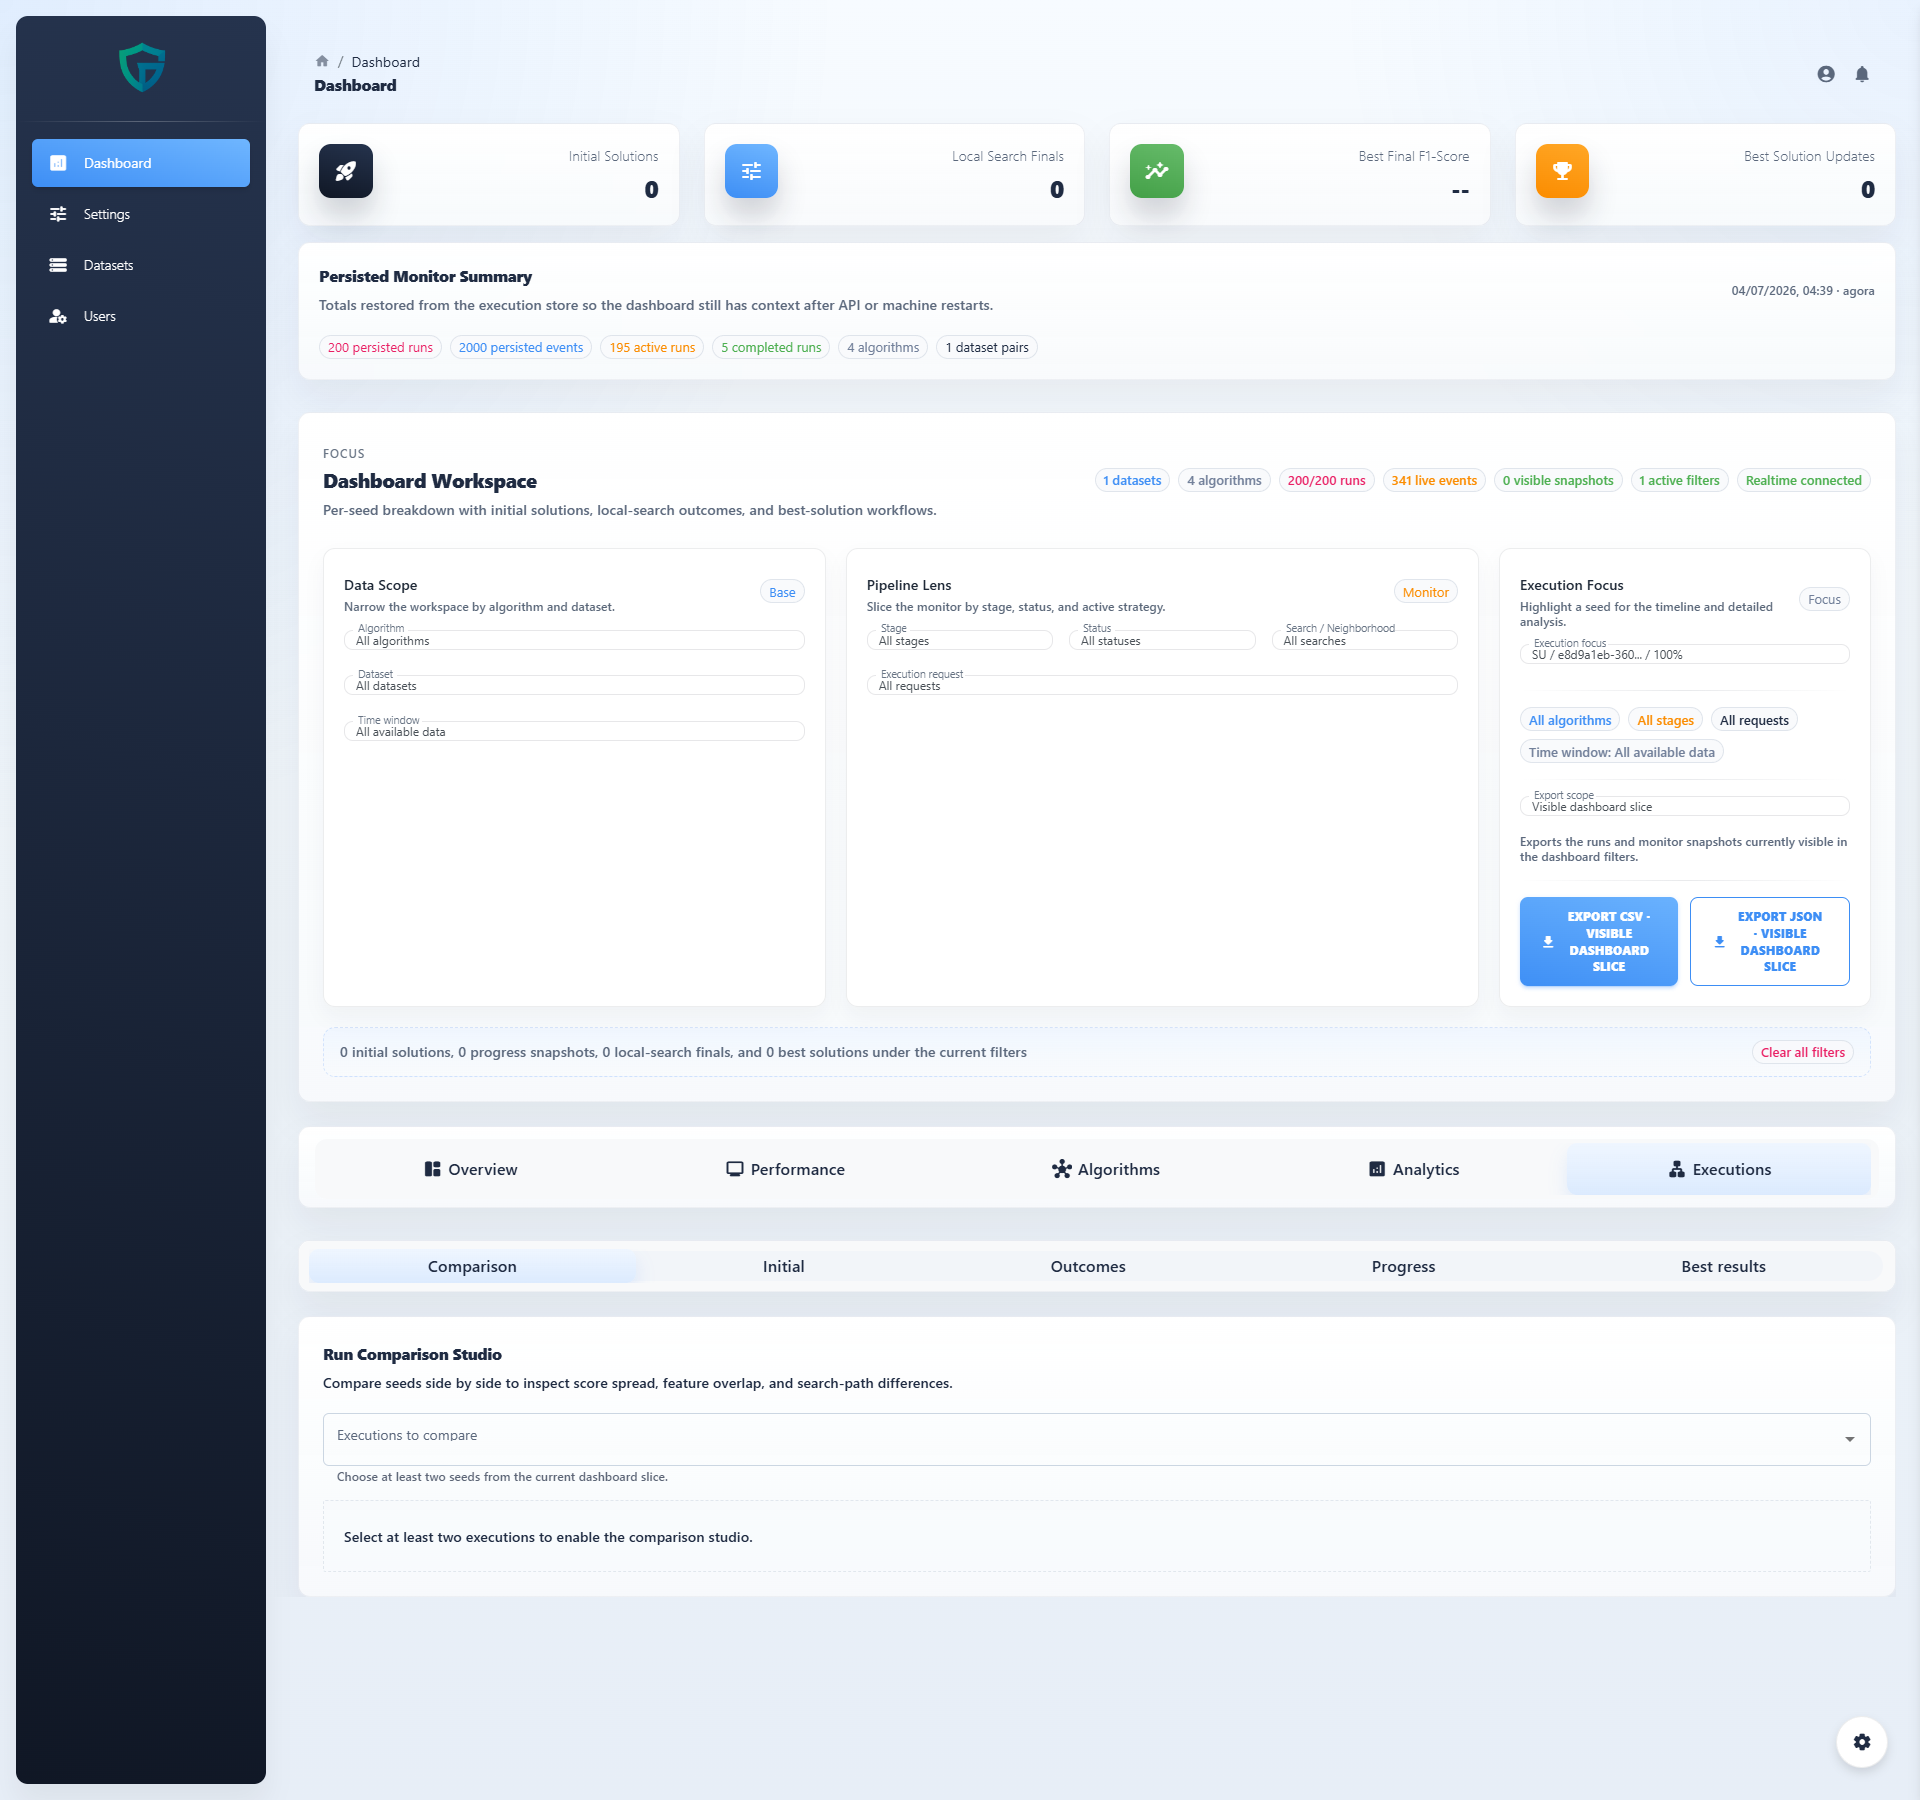
\includegraphics[width=\linewidth,height=0.80\textheight,keepaspectratio]{fig/front/08-dashboard-executions-comparison.png}
  \caption{Run comparison screen.}
  \label{fig:app-front-executions-comparison}
\end{figure}

\begin{figure}[!htb]
  \centering
  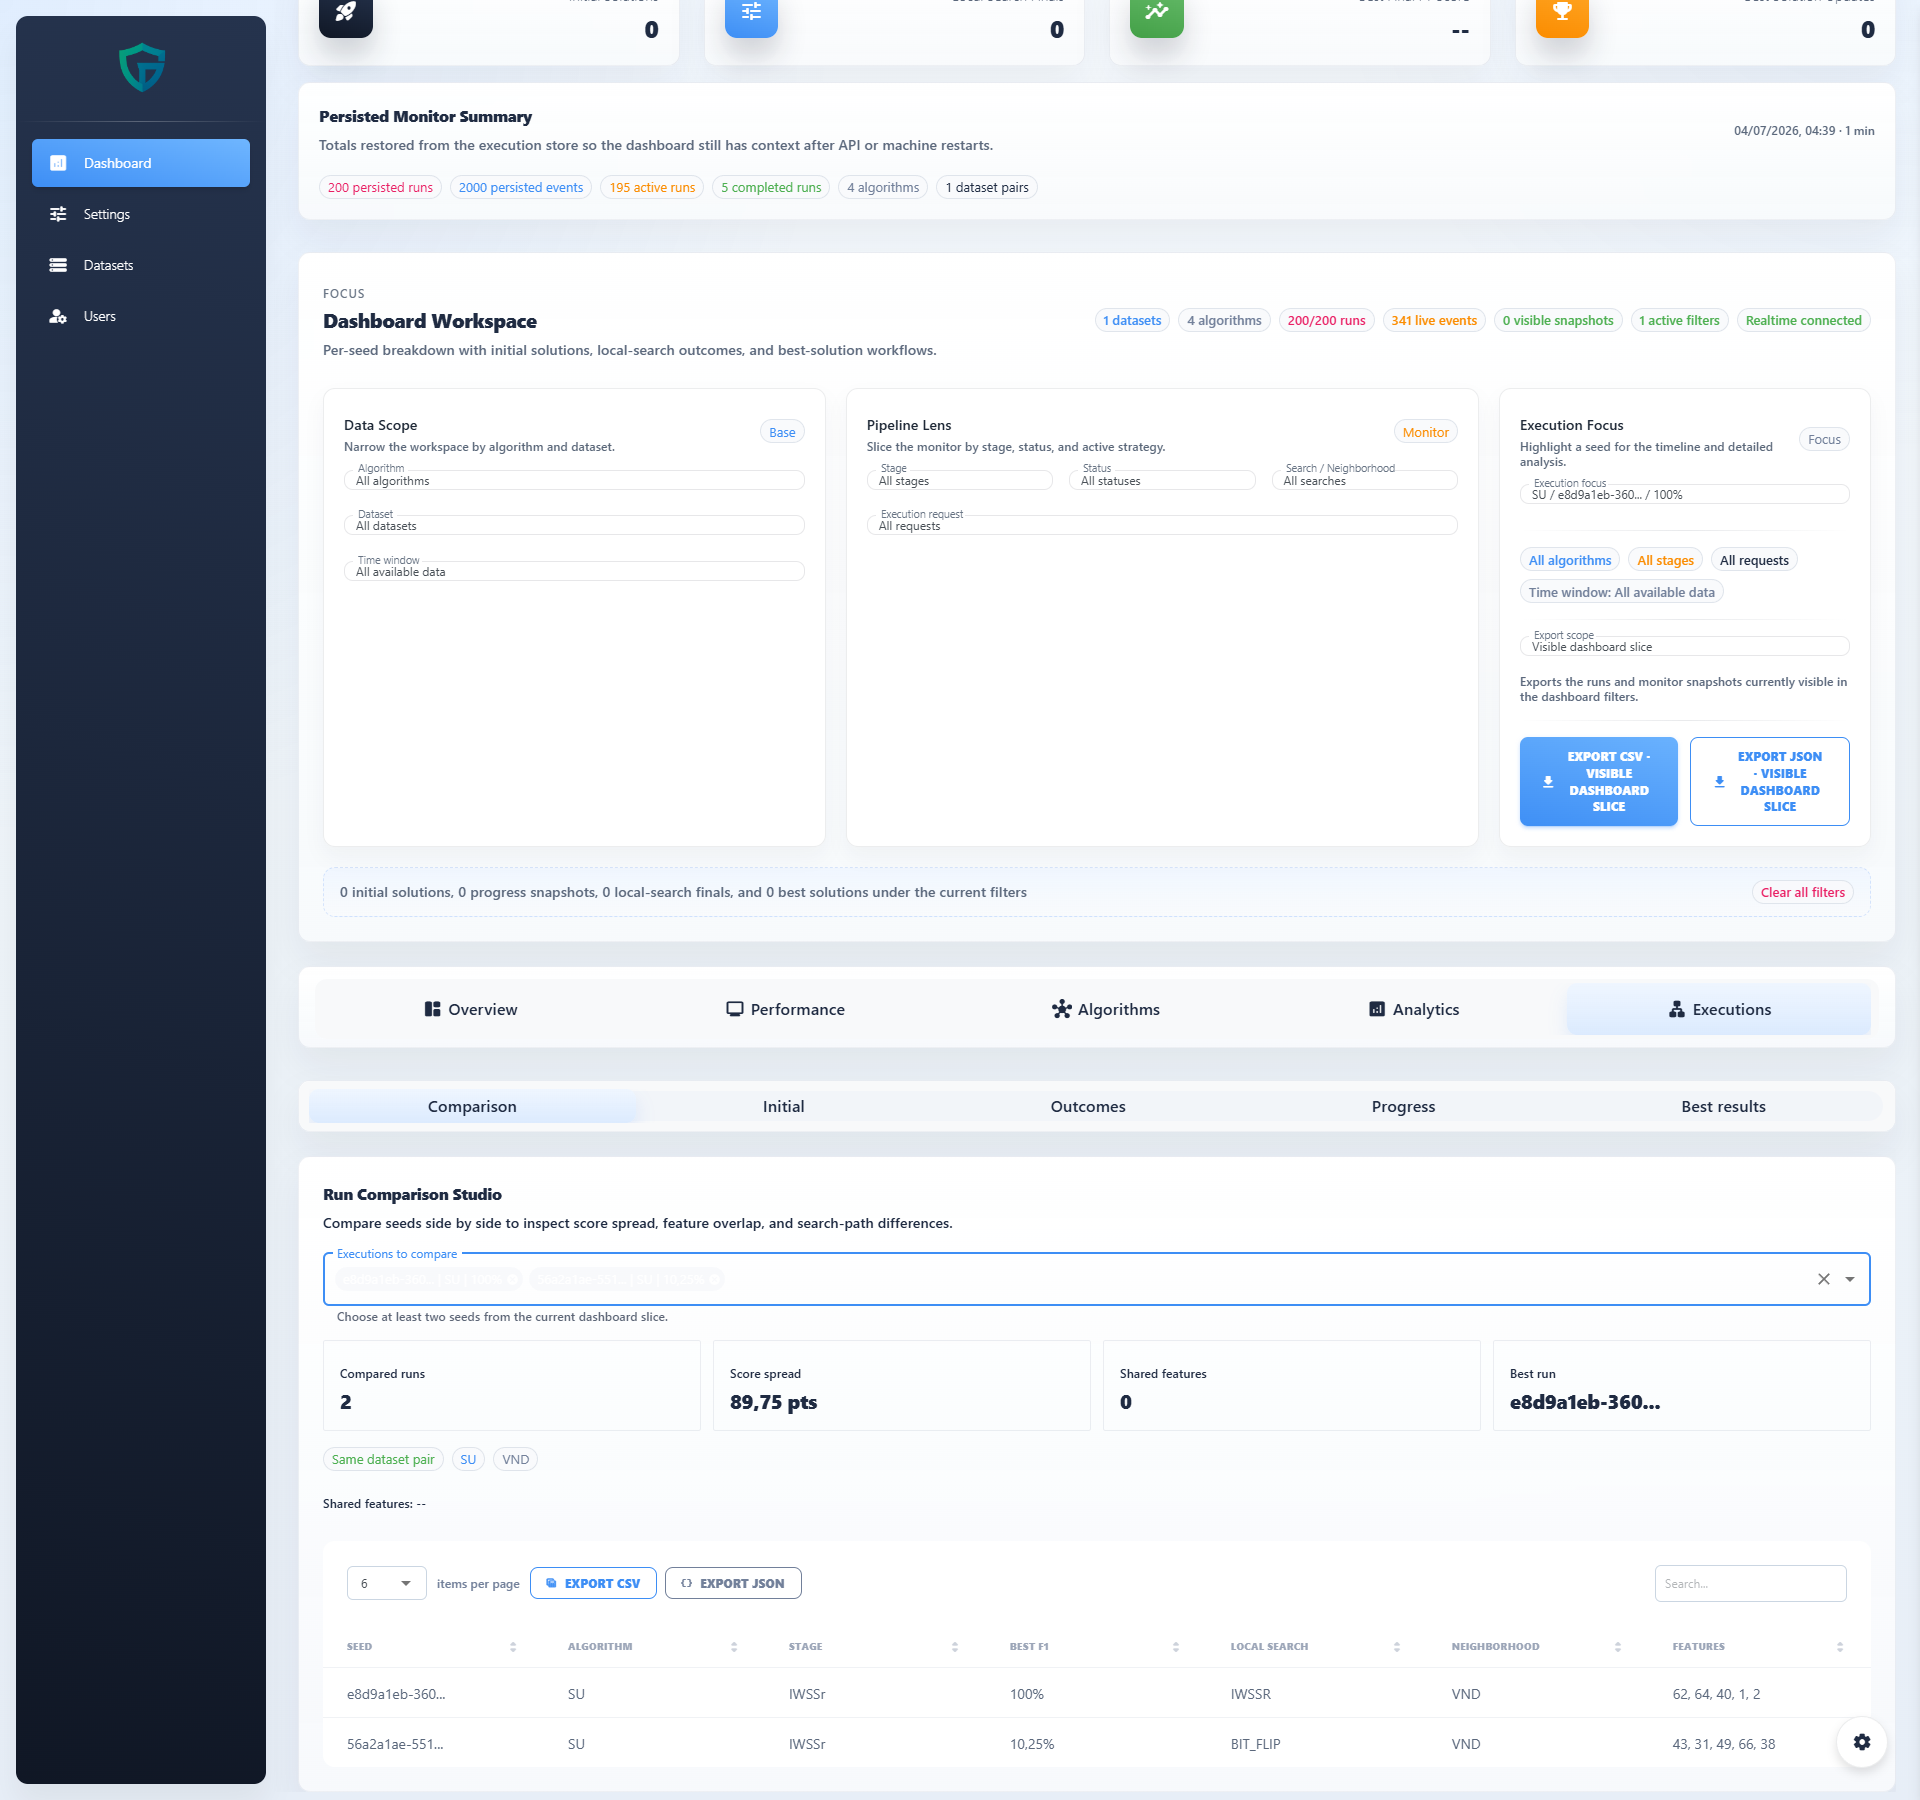
\includegraphics[width=\linewidth,height=0.80\textheight,keepaspectratio]{fig/front/13-dashboard-executions-comparison-selected.png}
  \caption{Comparison with selected seeds.}
  \label{fig:app-front-executions-comparison-selected}
\end{figure}

\begin{figure}[!htb]
  \centering
  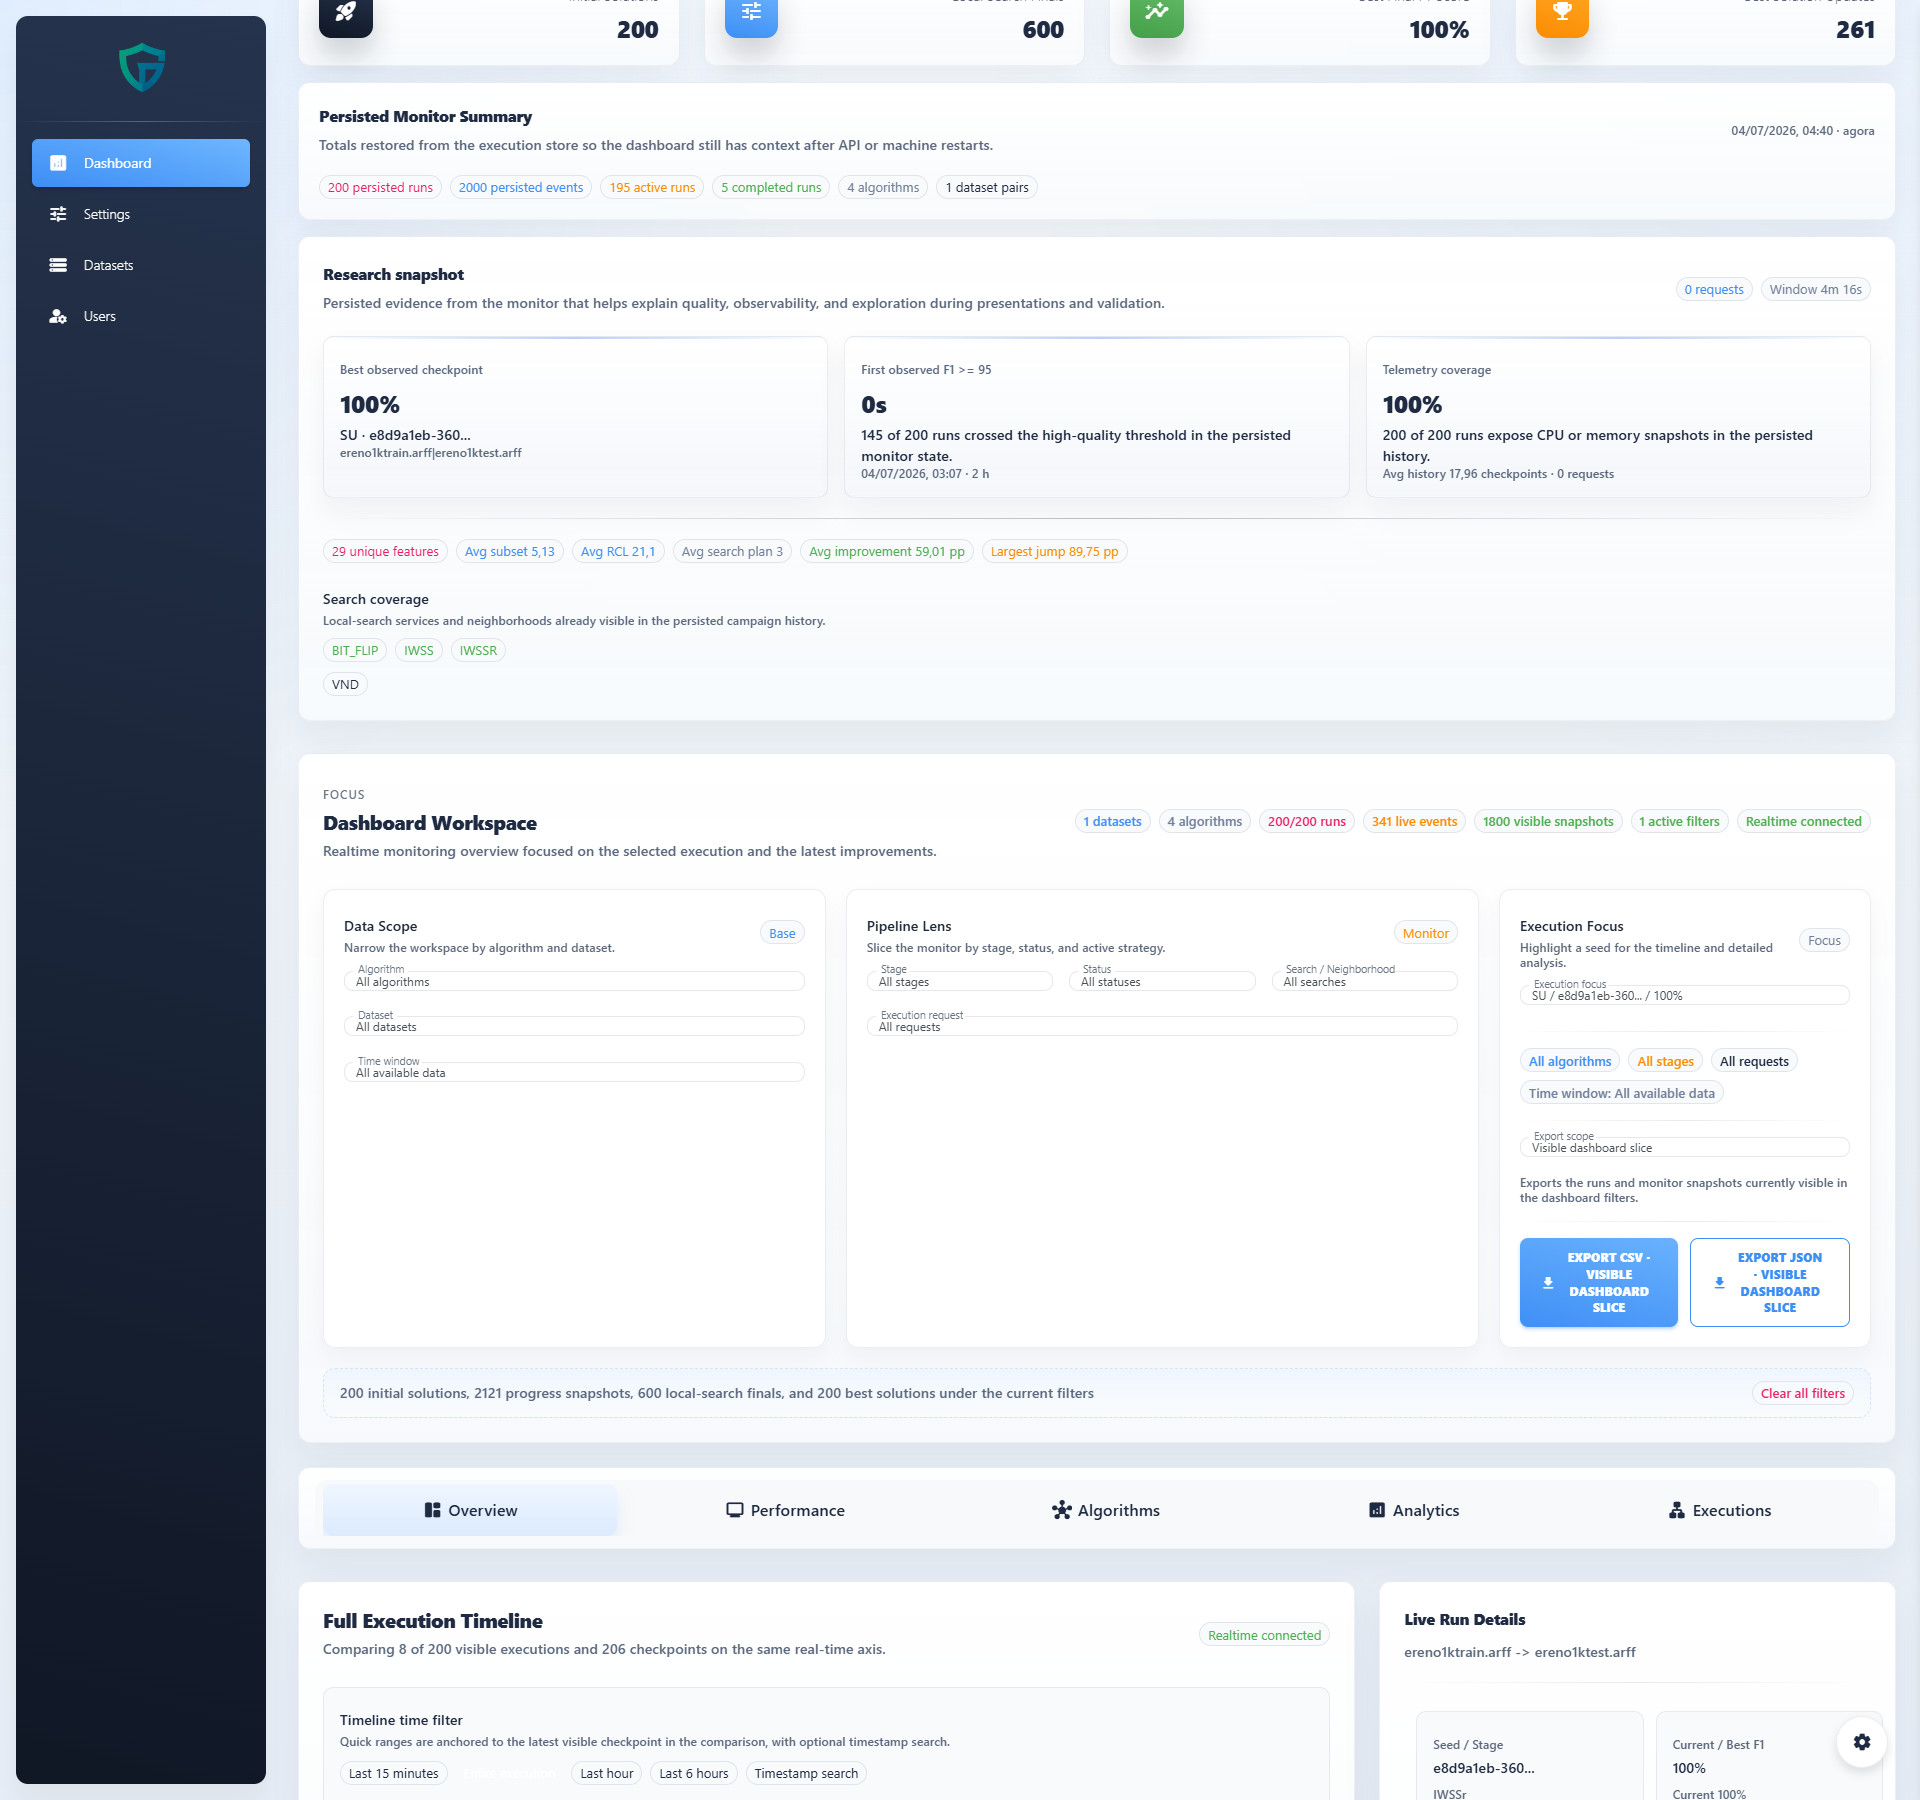
\includegraphics[width=\linewidth,height=0.80\textheight,keepaspectratio]{fig/front/14-dashboard-run-details.png}
  \caption{Details of a specific run.}
  \label{fig:app-front-run-details}
\end{figure}

\clearpage
\section{Timeline and Results}

The captures in this section show how the frontend presents the evolution of solutions over time, supporting interpretation of execution progress and quality.
Figures~\ref{fig:app-front-executions-initial},~\ref{fig:app-front-executions-outcomes},~\ref{fig:app-front-executions-progress}, and~\ref{fig:app-front-executions-best} complete that visual cycle.

\begin{figure}[!htb]
  \centering
  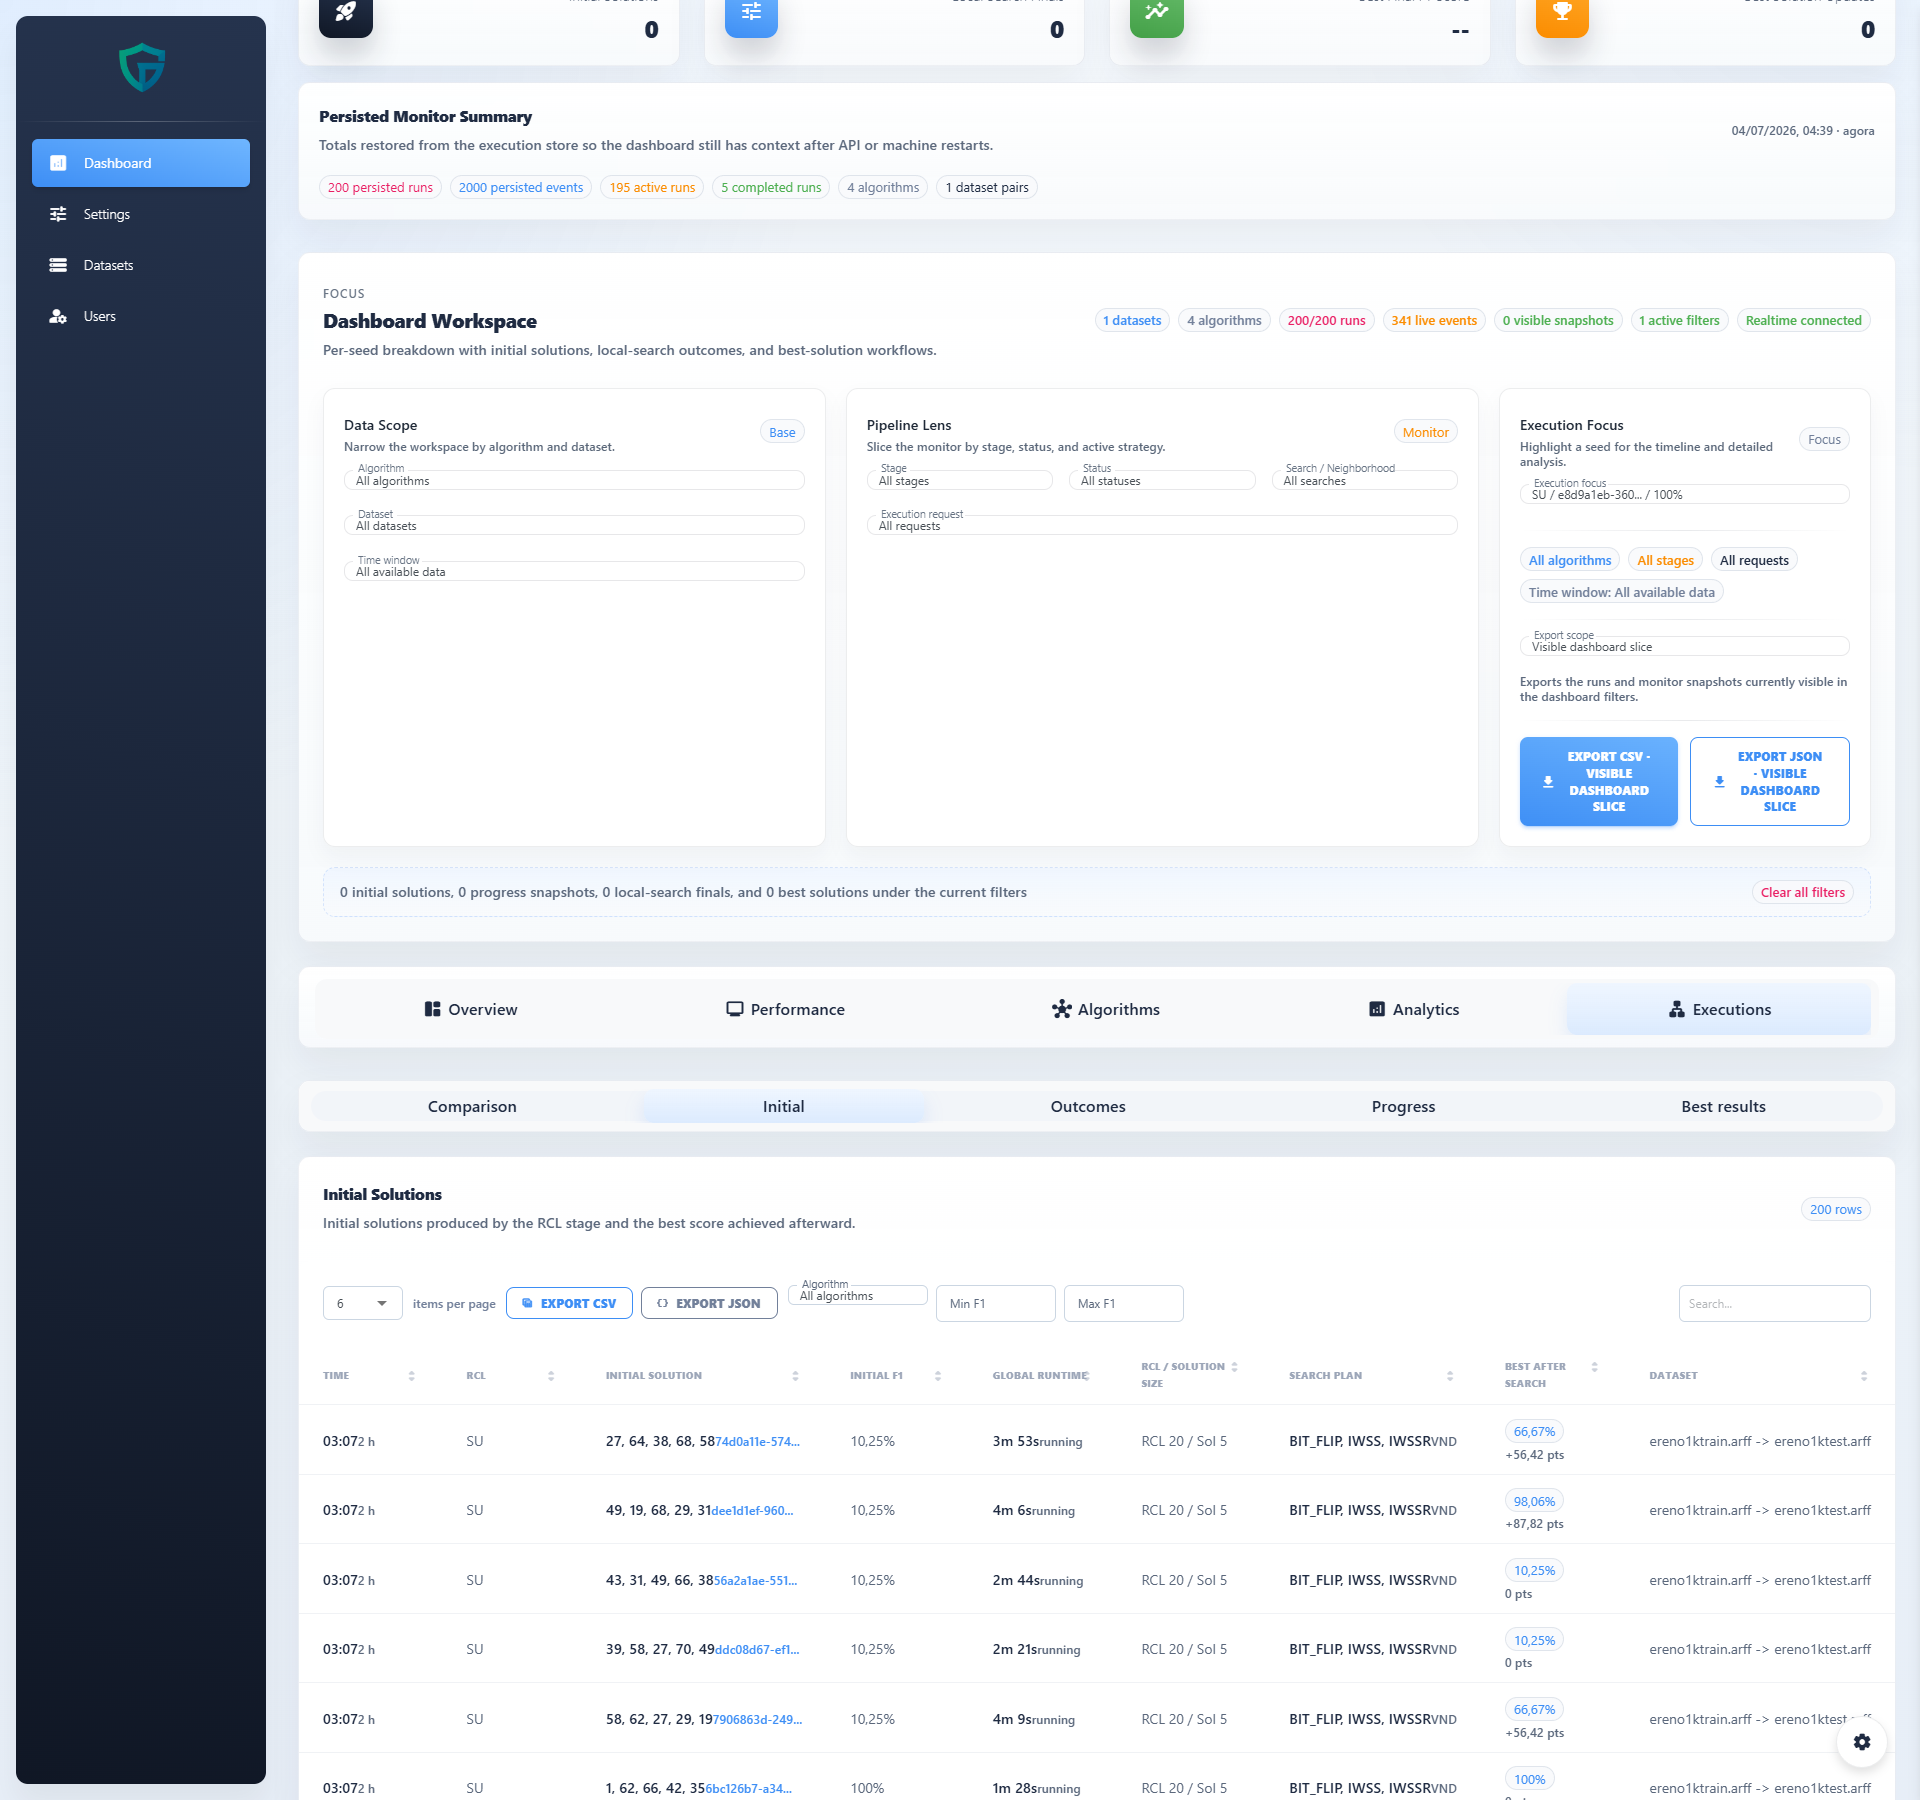
\includegraphics[width=\linewidth,height=0.80\textheight,keepaspectratio]{fig/front/09-dashboard-executions-initial.png}
  \caption{Initial solutions.}
  \label{fig:app-front-executions-initial}
\end{figure}

\begin{figure}[!htb]
  \centering
  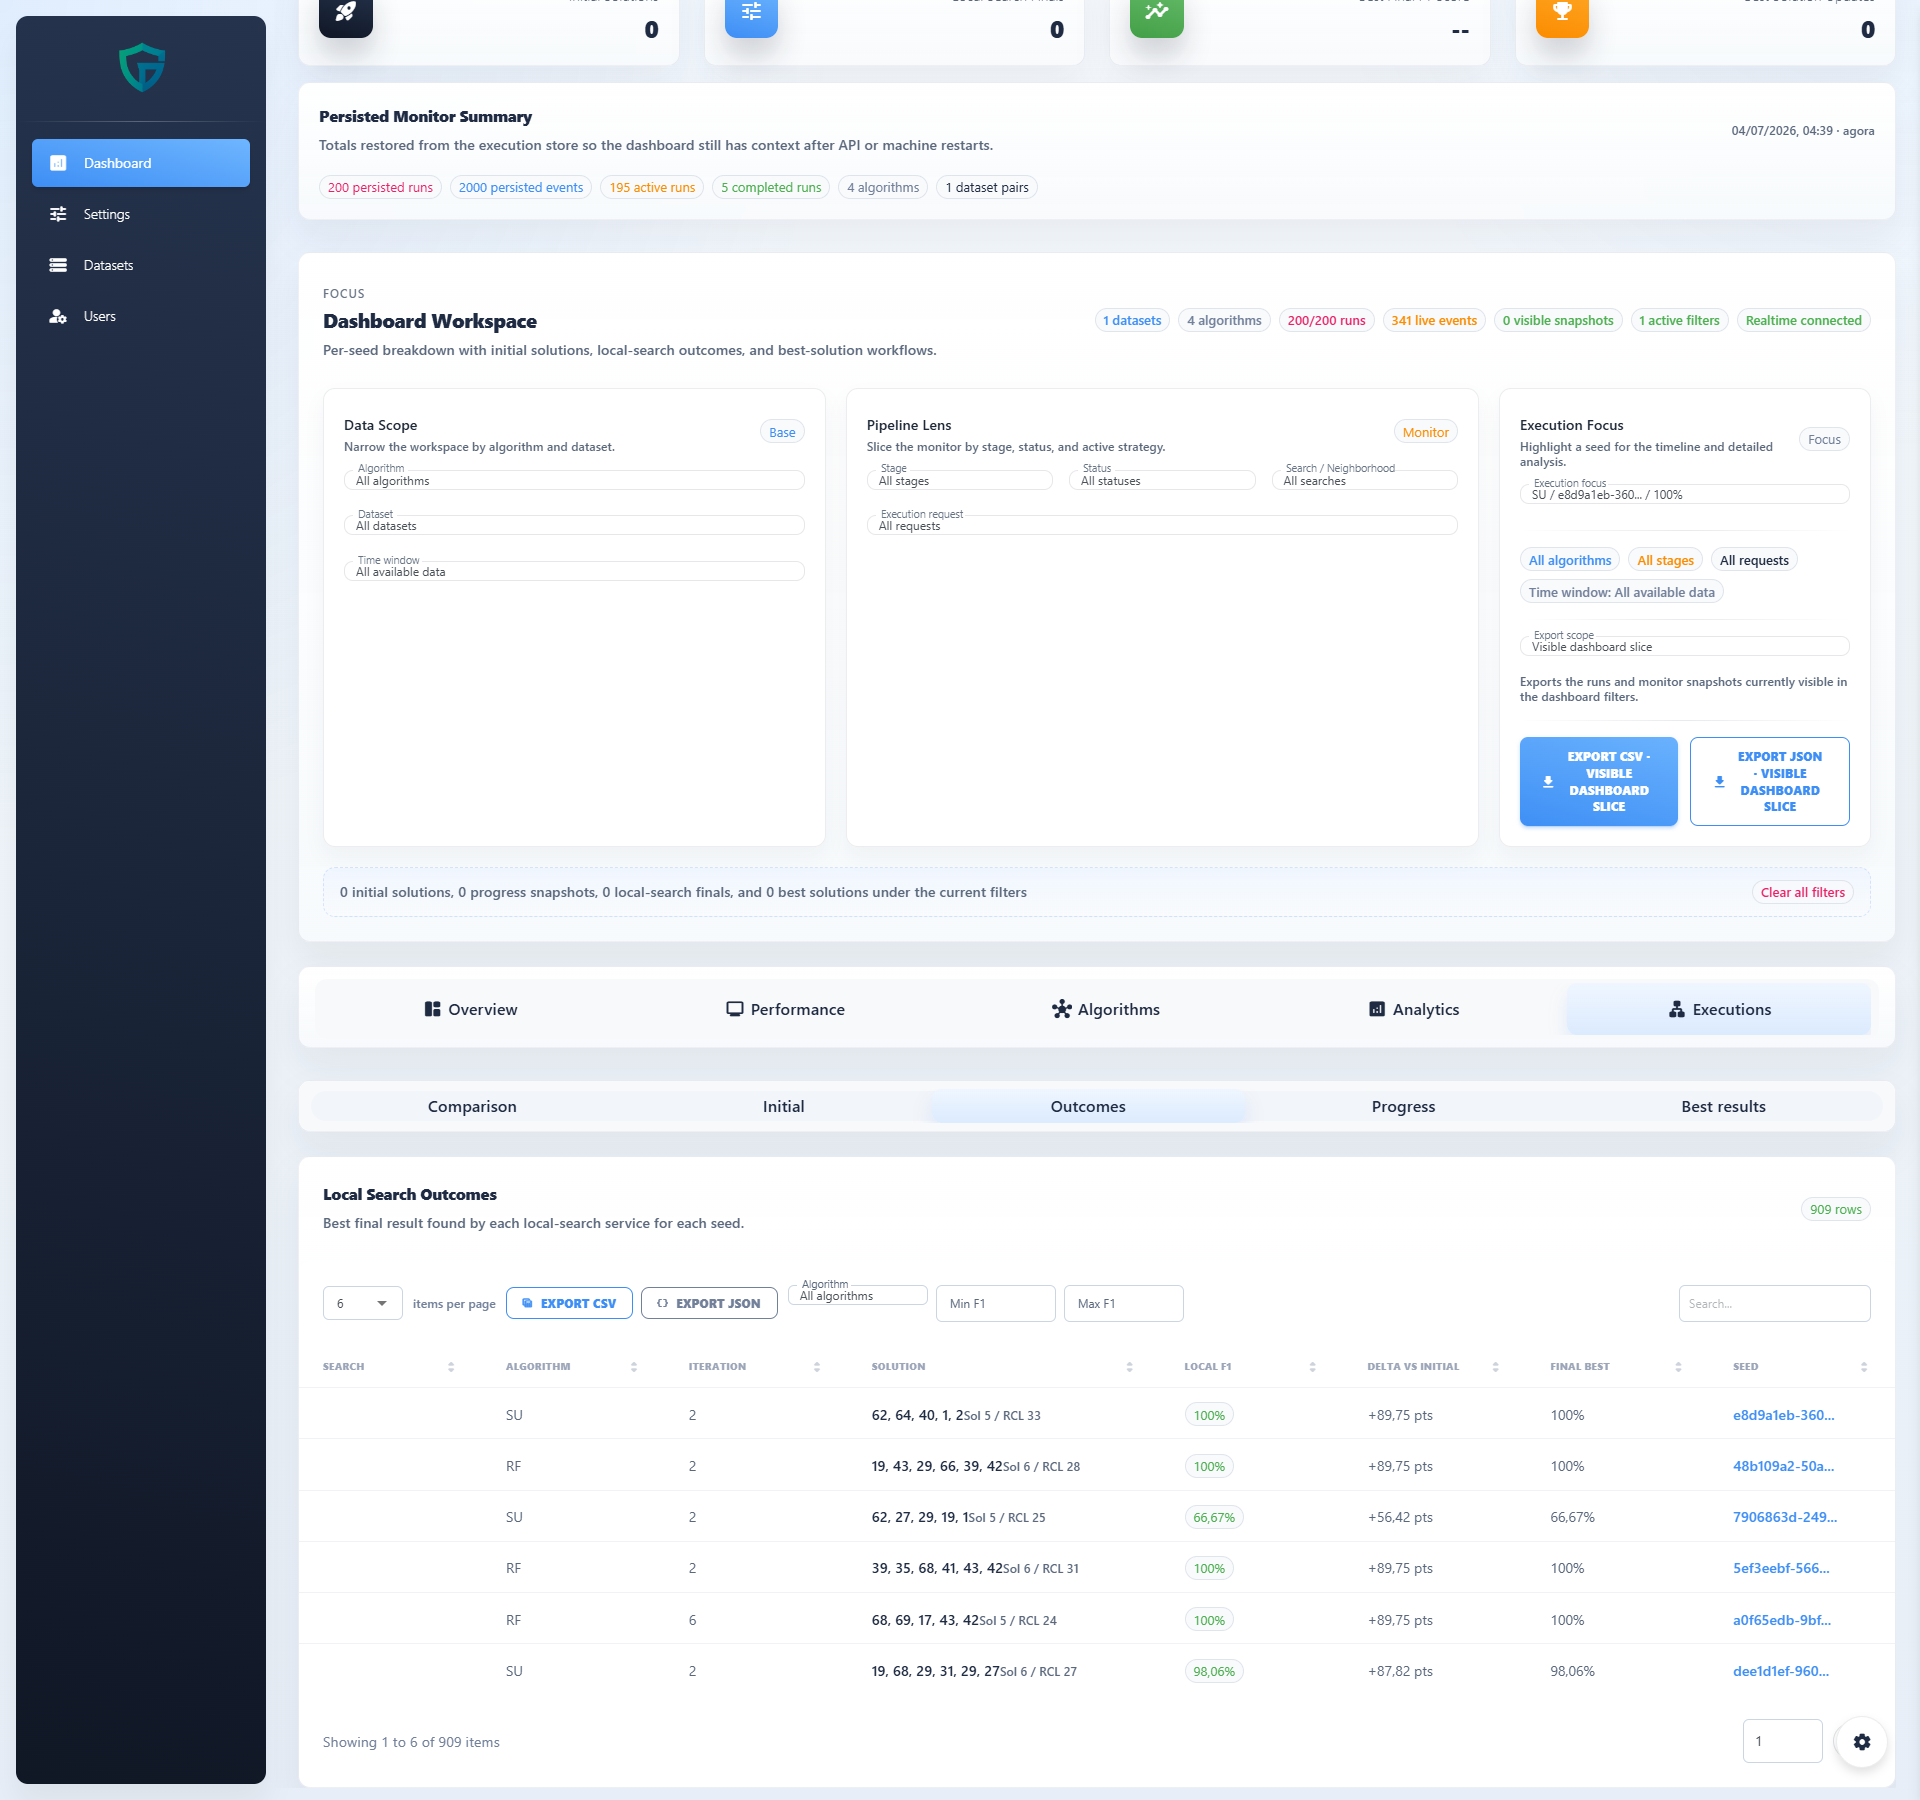
\includegraphics[width=\linewidth,height=0.80\textheight,keepaspectratio]{fig/front/10-dashboard-executions-outcomes.png}
  \caption{Consolidated outcomes.}
  \label{fig:app-front-executions-outcomes}
\end{figure}

\begin{figure}[!htb]
  \centering
  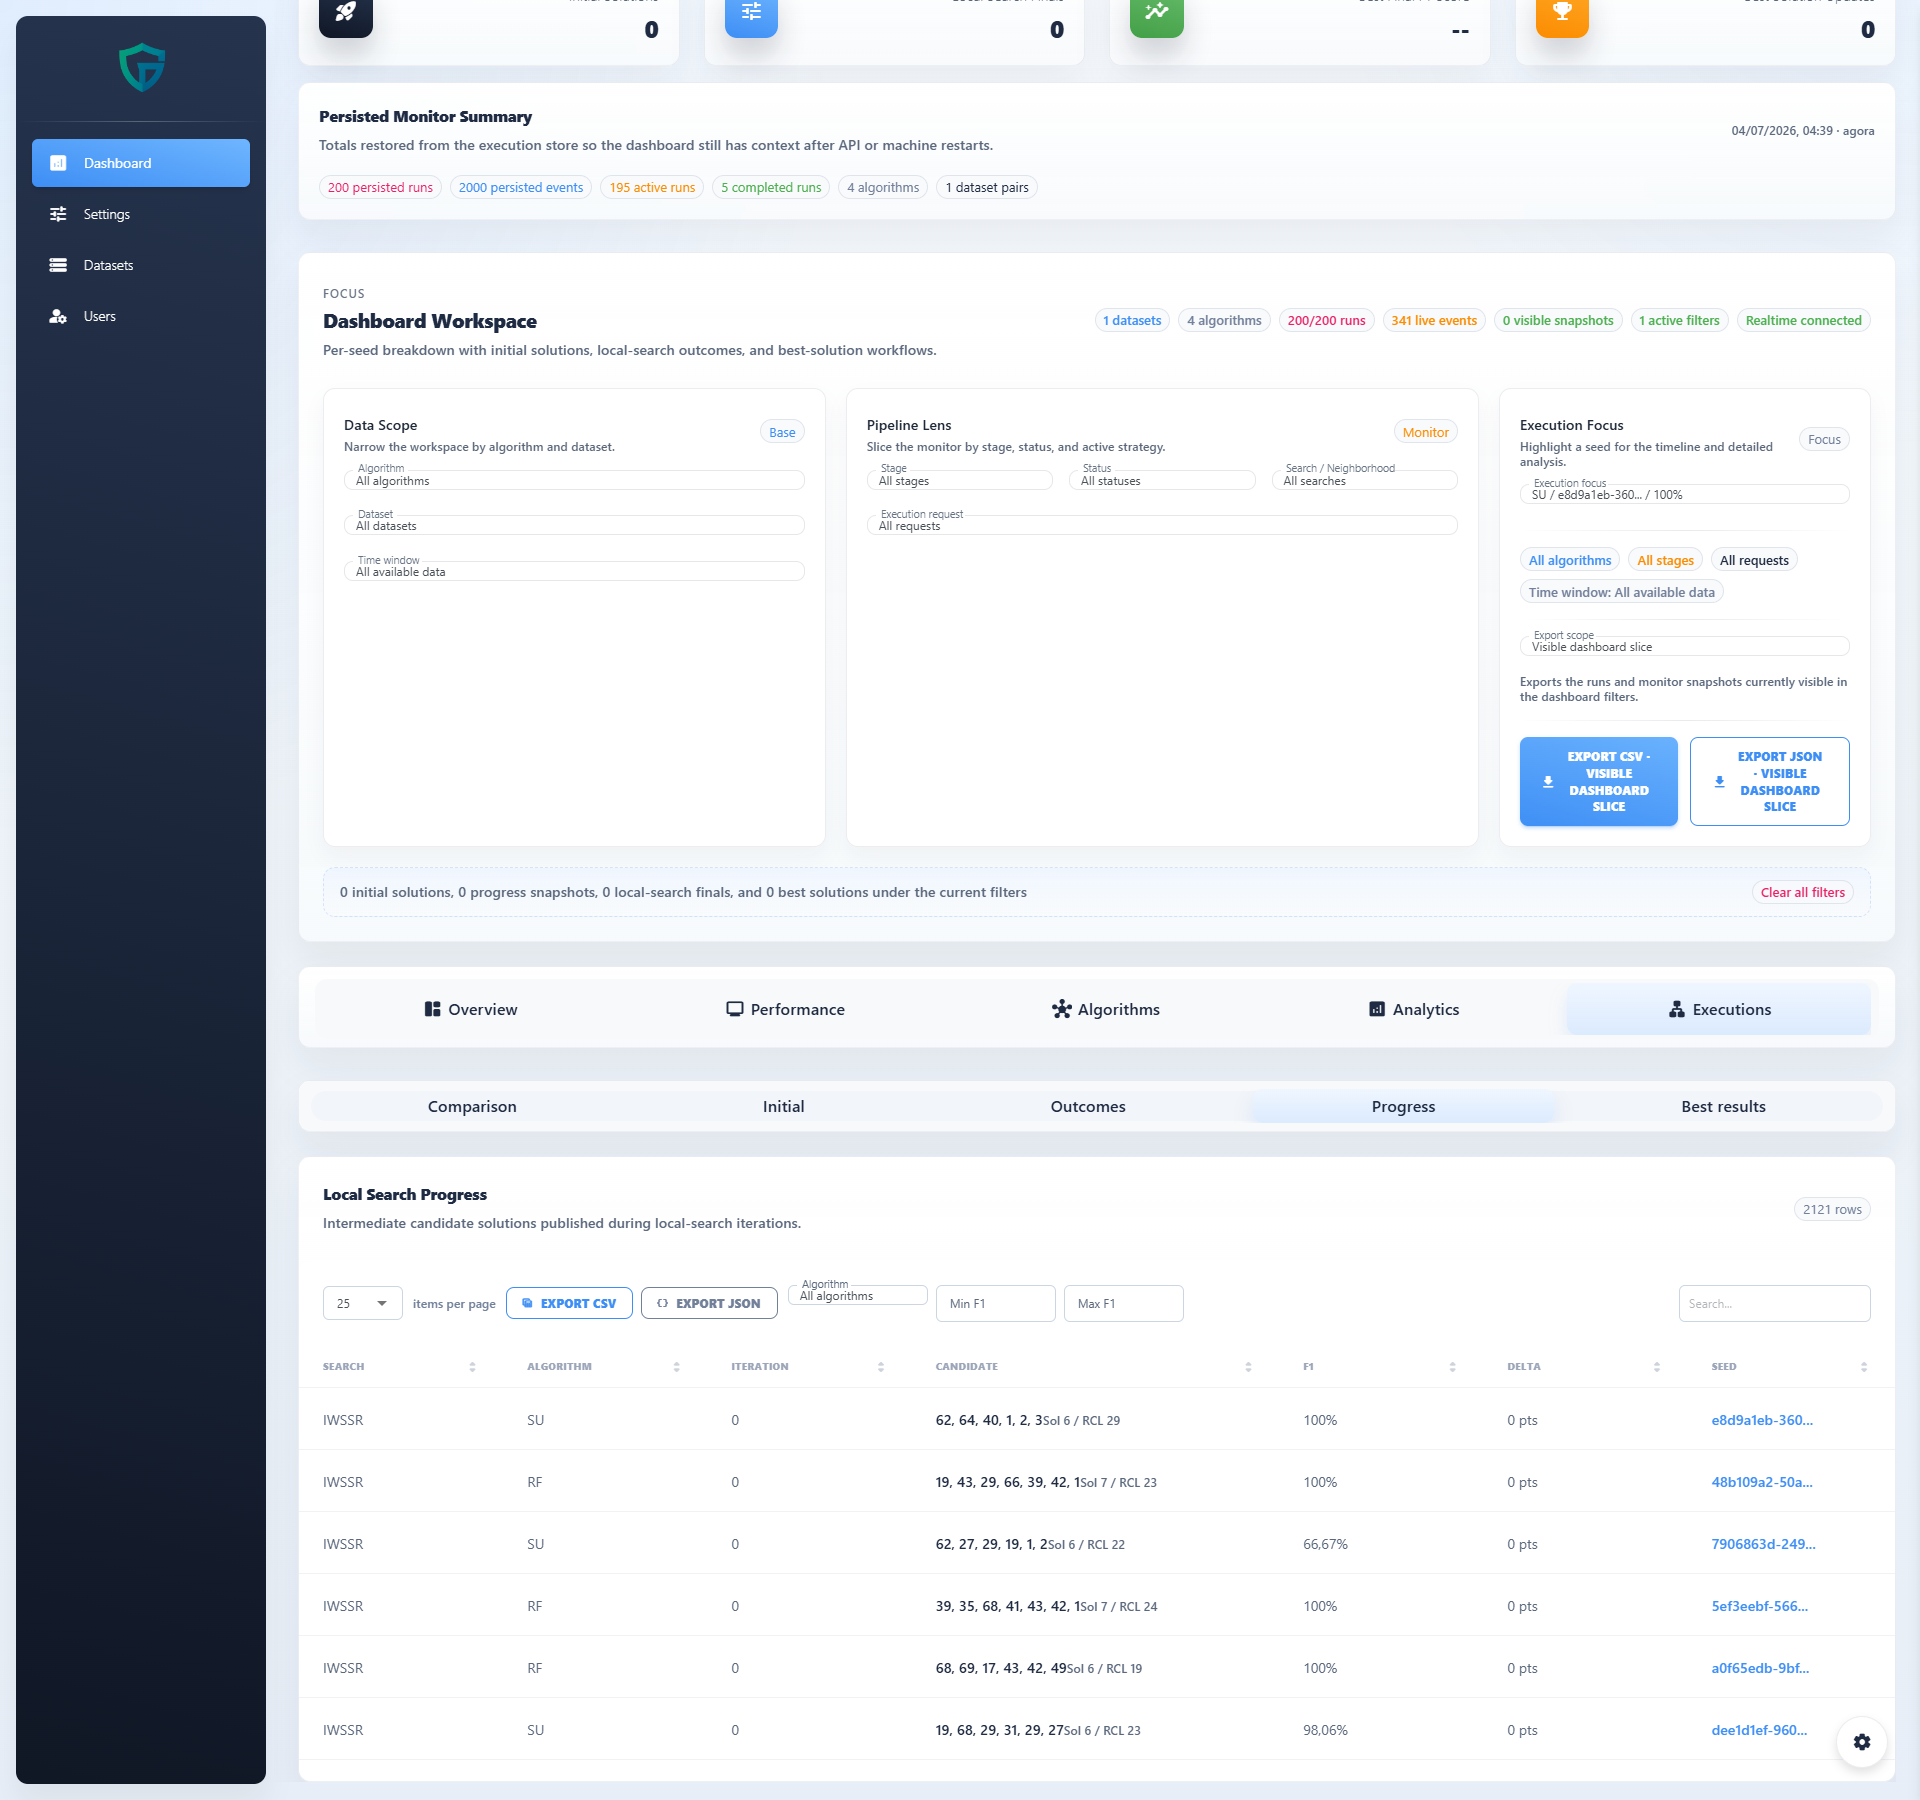
\includegraphics[width=\linewidth,height=0.80\textheight,keepaspectratio]{fig/front/11-dashboard-executions-progress.png}
  \caption{Execution progress.}
  \label{fig:app-front-executions-progress}
\end{figure}

\begin{figure}[!htb]
  \centering
  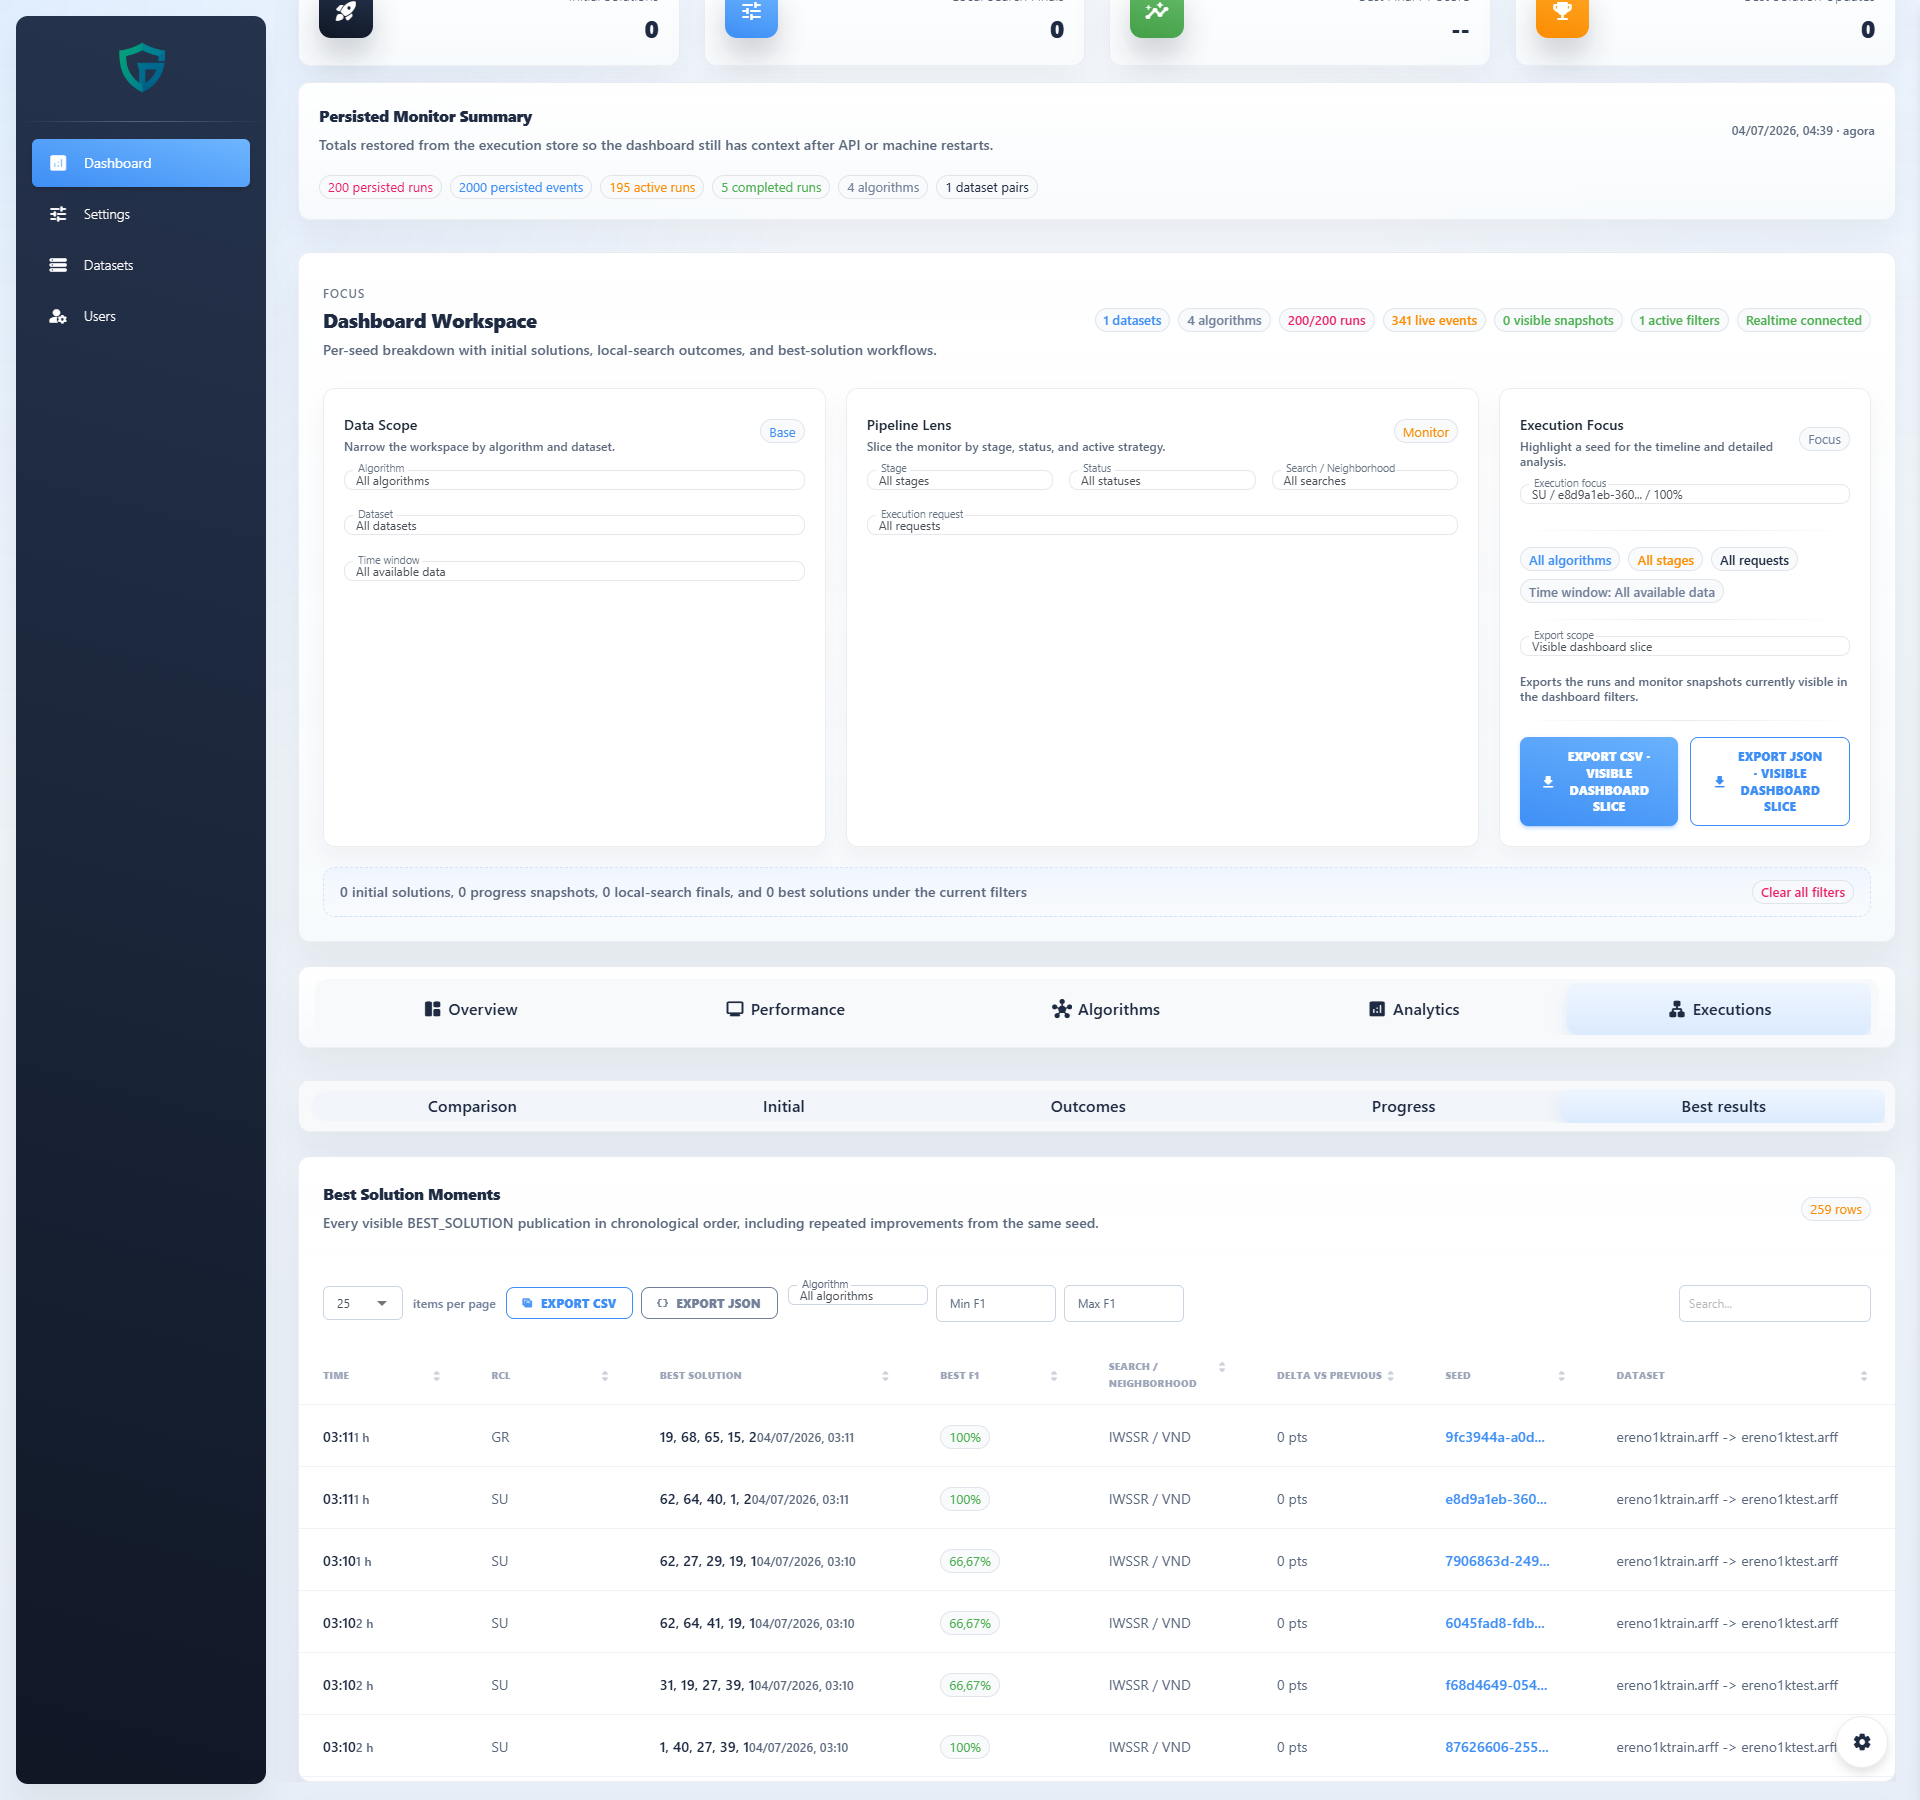
\includegraphics[width=\linewidth,height=0.80\textheight,keepaspectratio]{fig/front/12-dashboard-executions-best.png}
  \caption{Best solutions.}
  \label{fig:app-front-executions-best}
\end{figure}

\clearpage
\section{Settings and Administration}

Finally, the administrative screens show that the platform also covers operation and maintenance aspects, and Figures~\ref{fig:app-front-settings-execution},~\ref{fig:app-front-settings-datasets},~\ref{fig:app-front-settings-operations},~\ref{fig:app-front-settings-reset},~\ref{fig:app-front-datasets},~\ref{fig:app-front-users-list}, and~\ref{fig:app-front-user-edit} show the administrative set.

\begin{figure}[!htb]
  \centering
  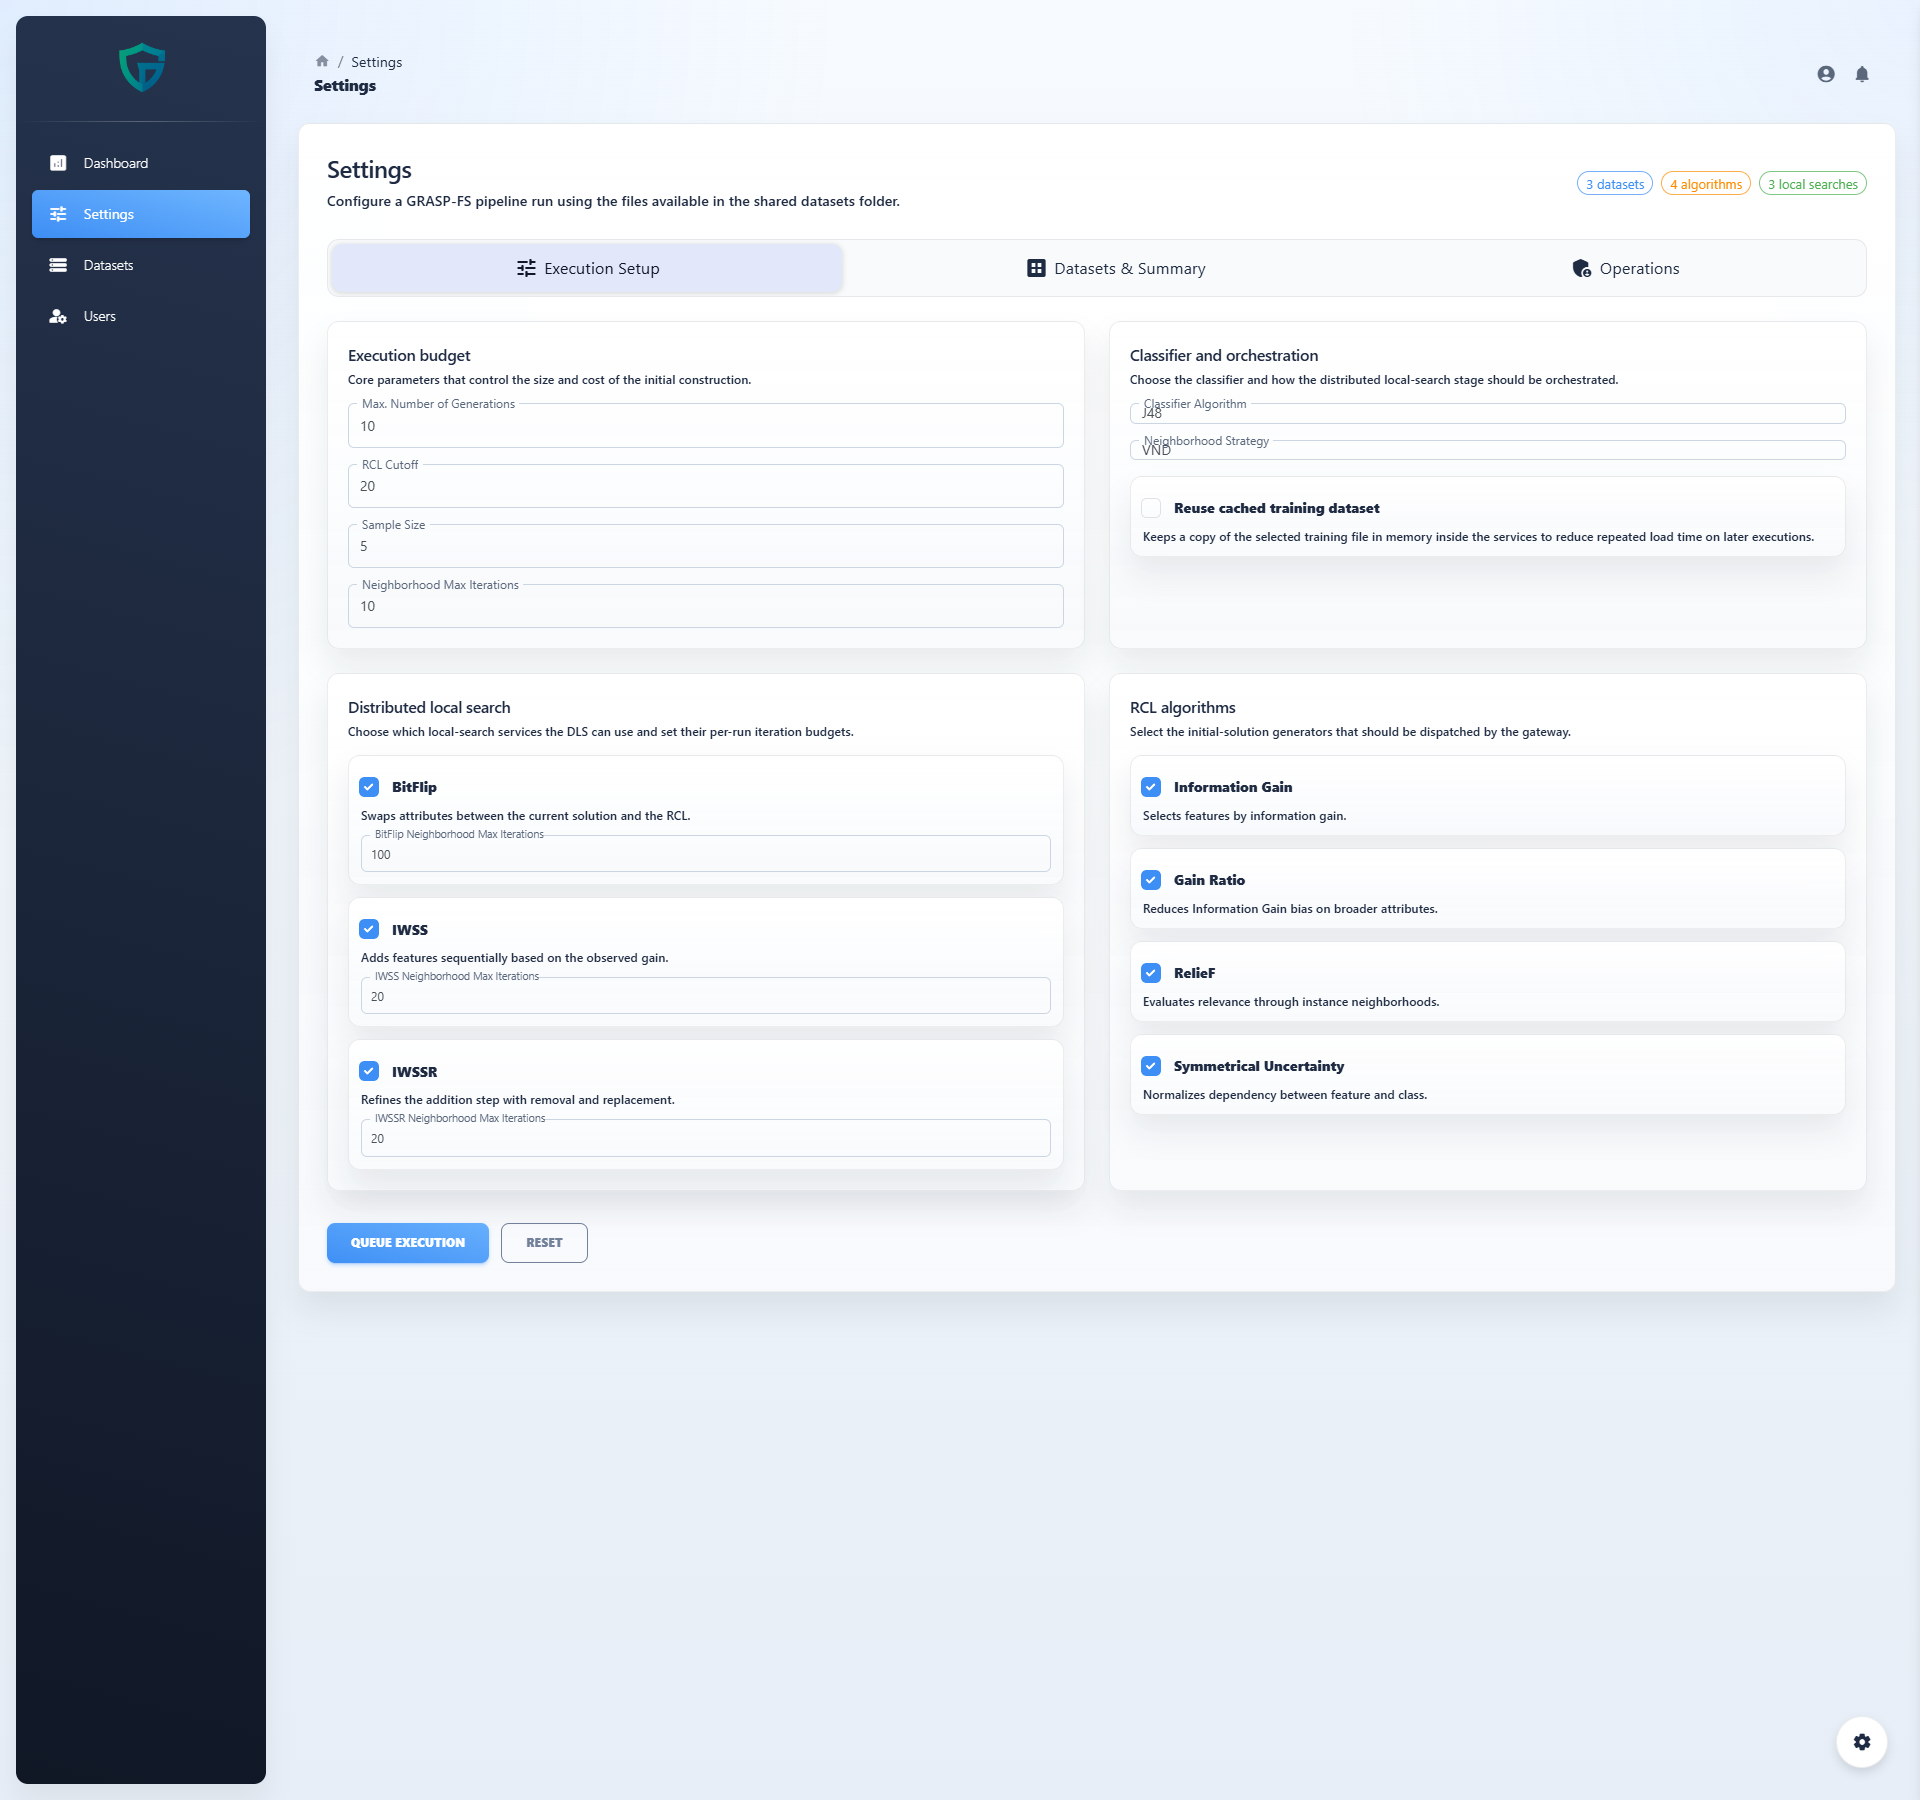
\includegraphics[width=\linewidth,height=0.80\textheight,keepaspectratio]{fig/front/15-settings-execution.png}
  \caption{Execution settings.}
  \label{fig:app-front-settings-execution}
\end{figure}

\begin{figure}[!htb]
  \centering
  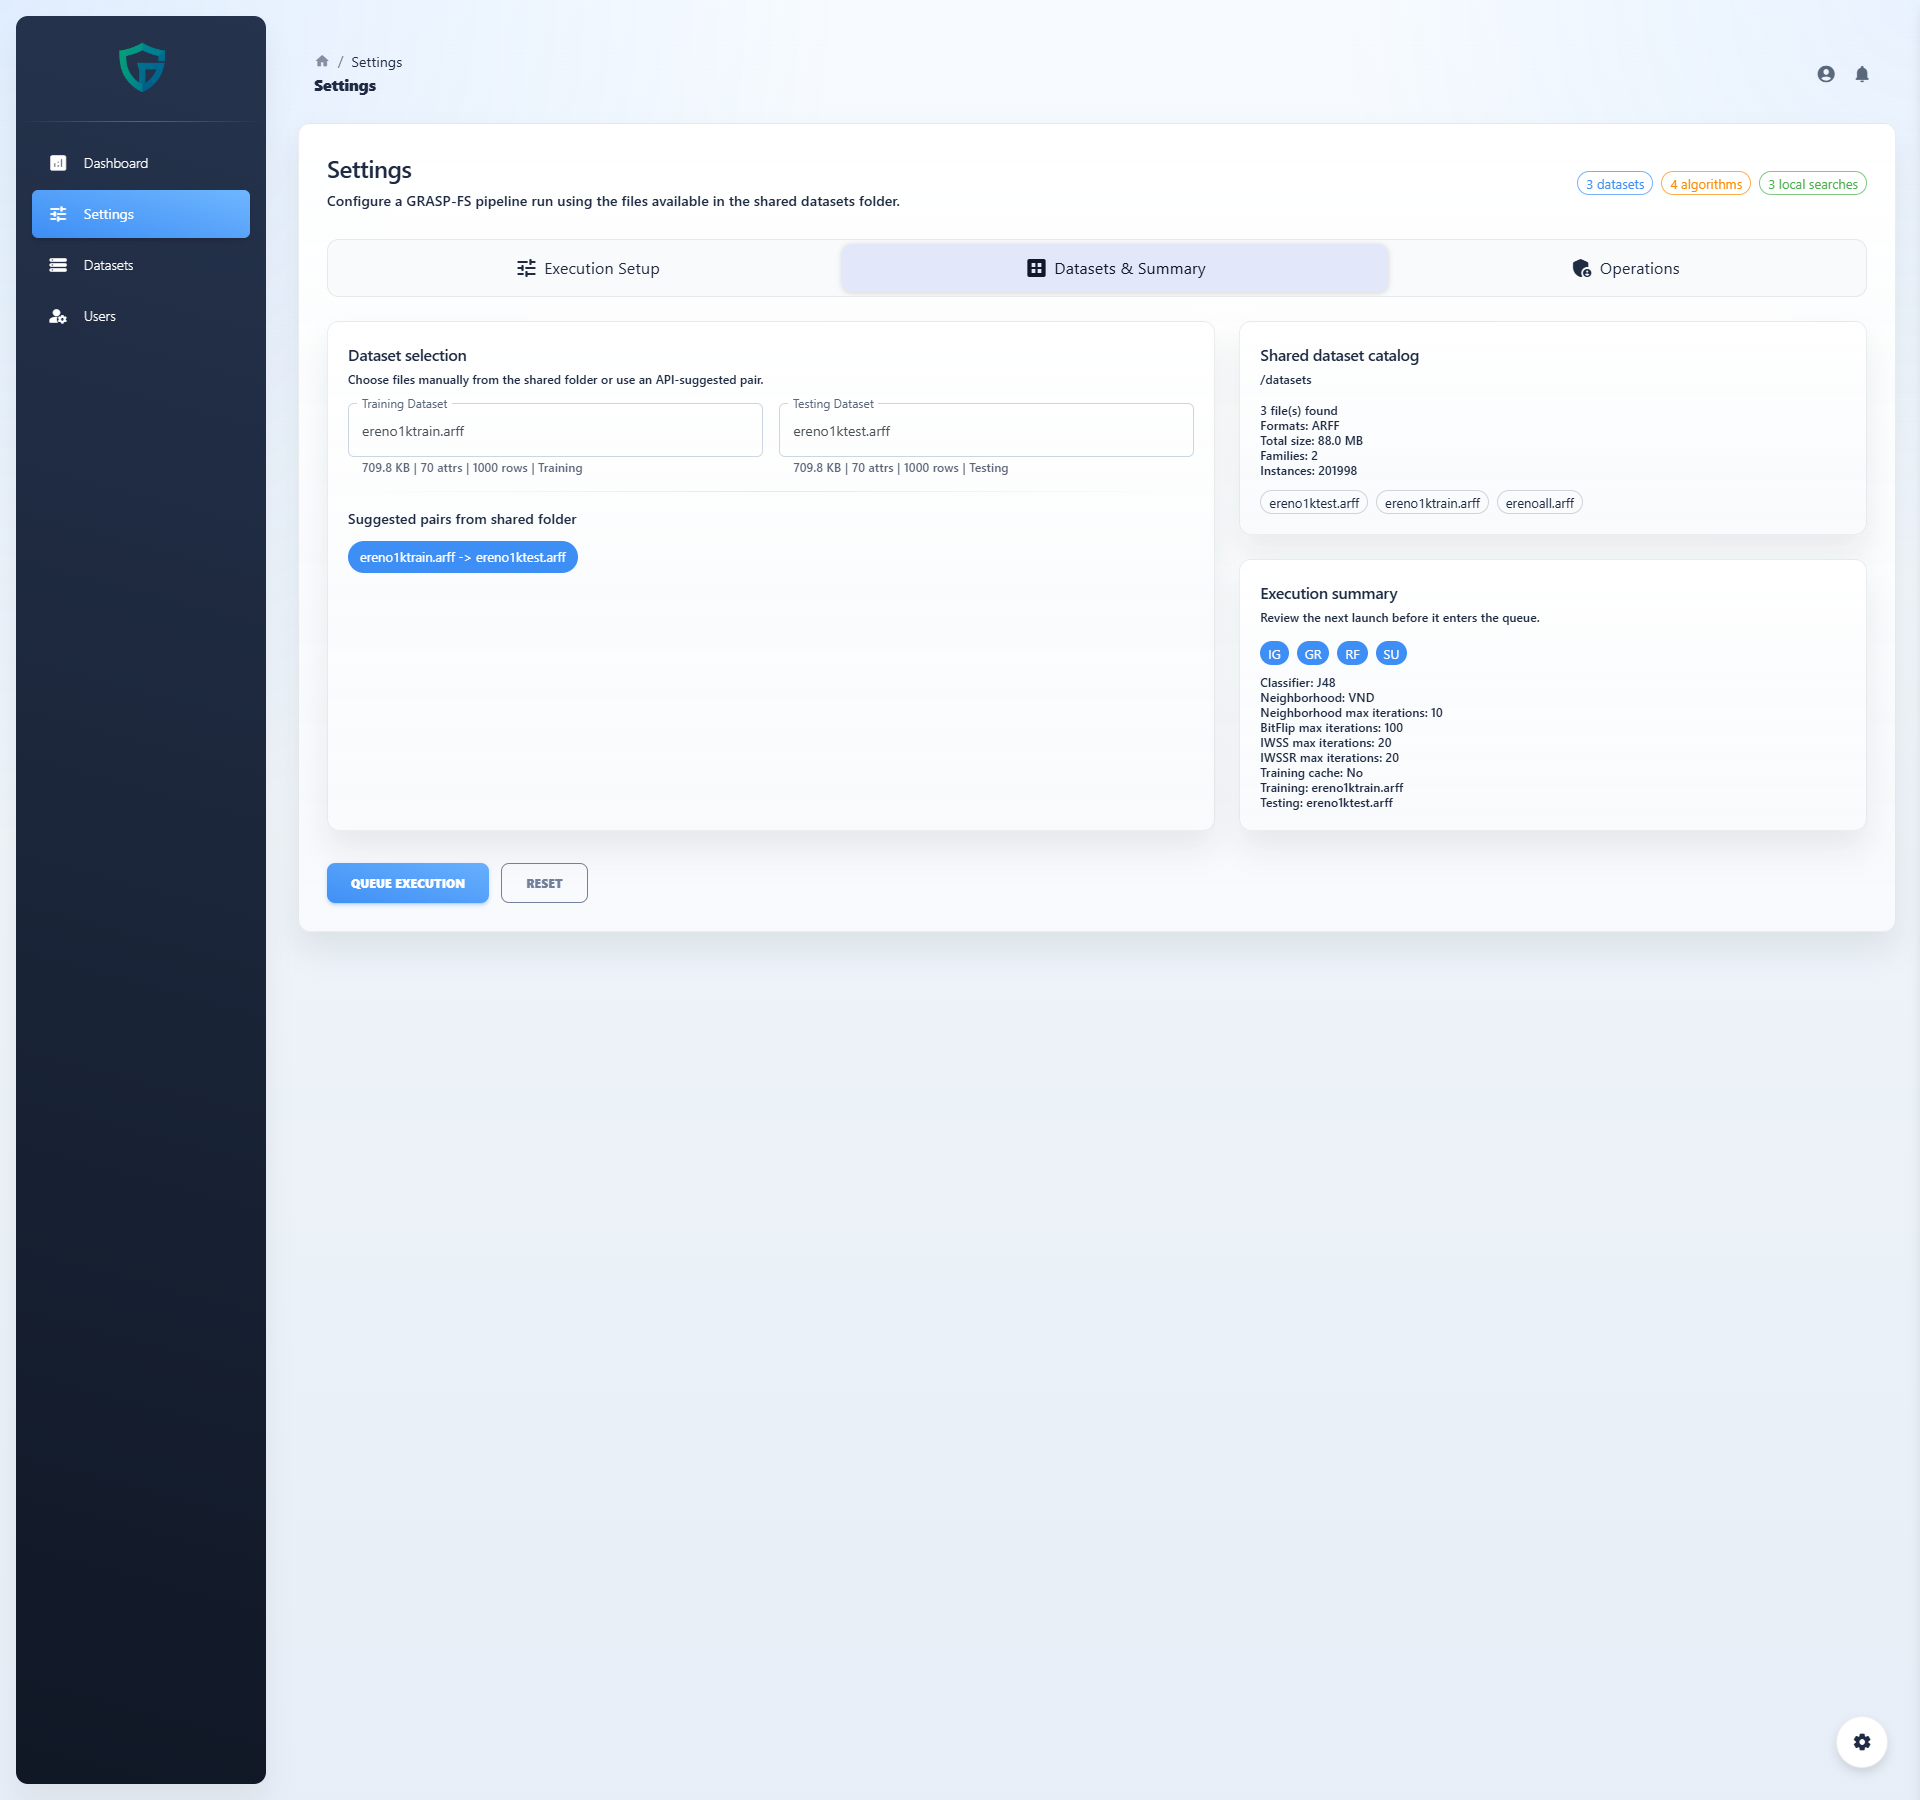
\includegraphics[width=\linewidth,height=0.80\textheight,keepaspectratio]{fig/front/16-settings-datasets.png}
  \caption{Dataset settings.}
  \label{fig:app-front-settings-datasets}
\end{figure}

\begin{figure}[!htb]
  \centering
  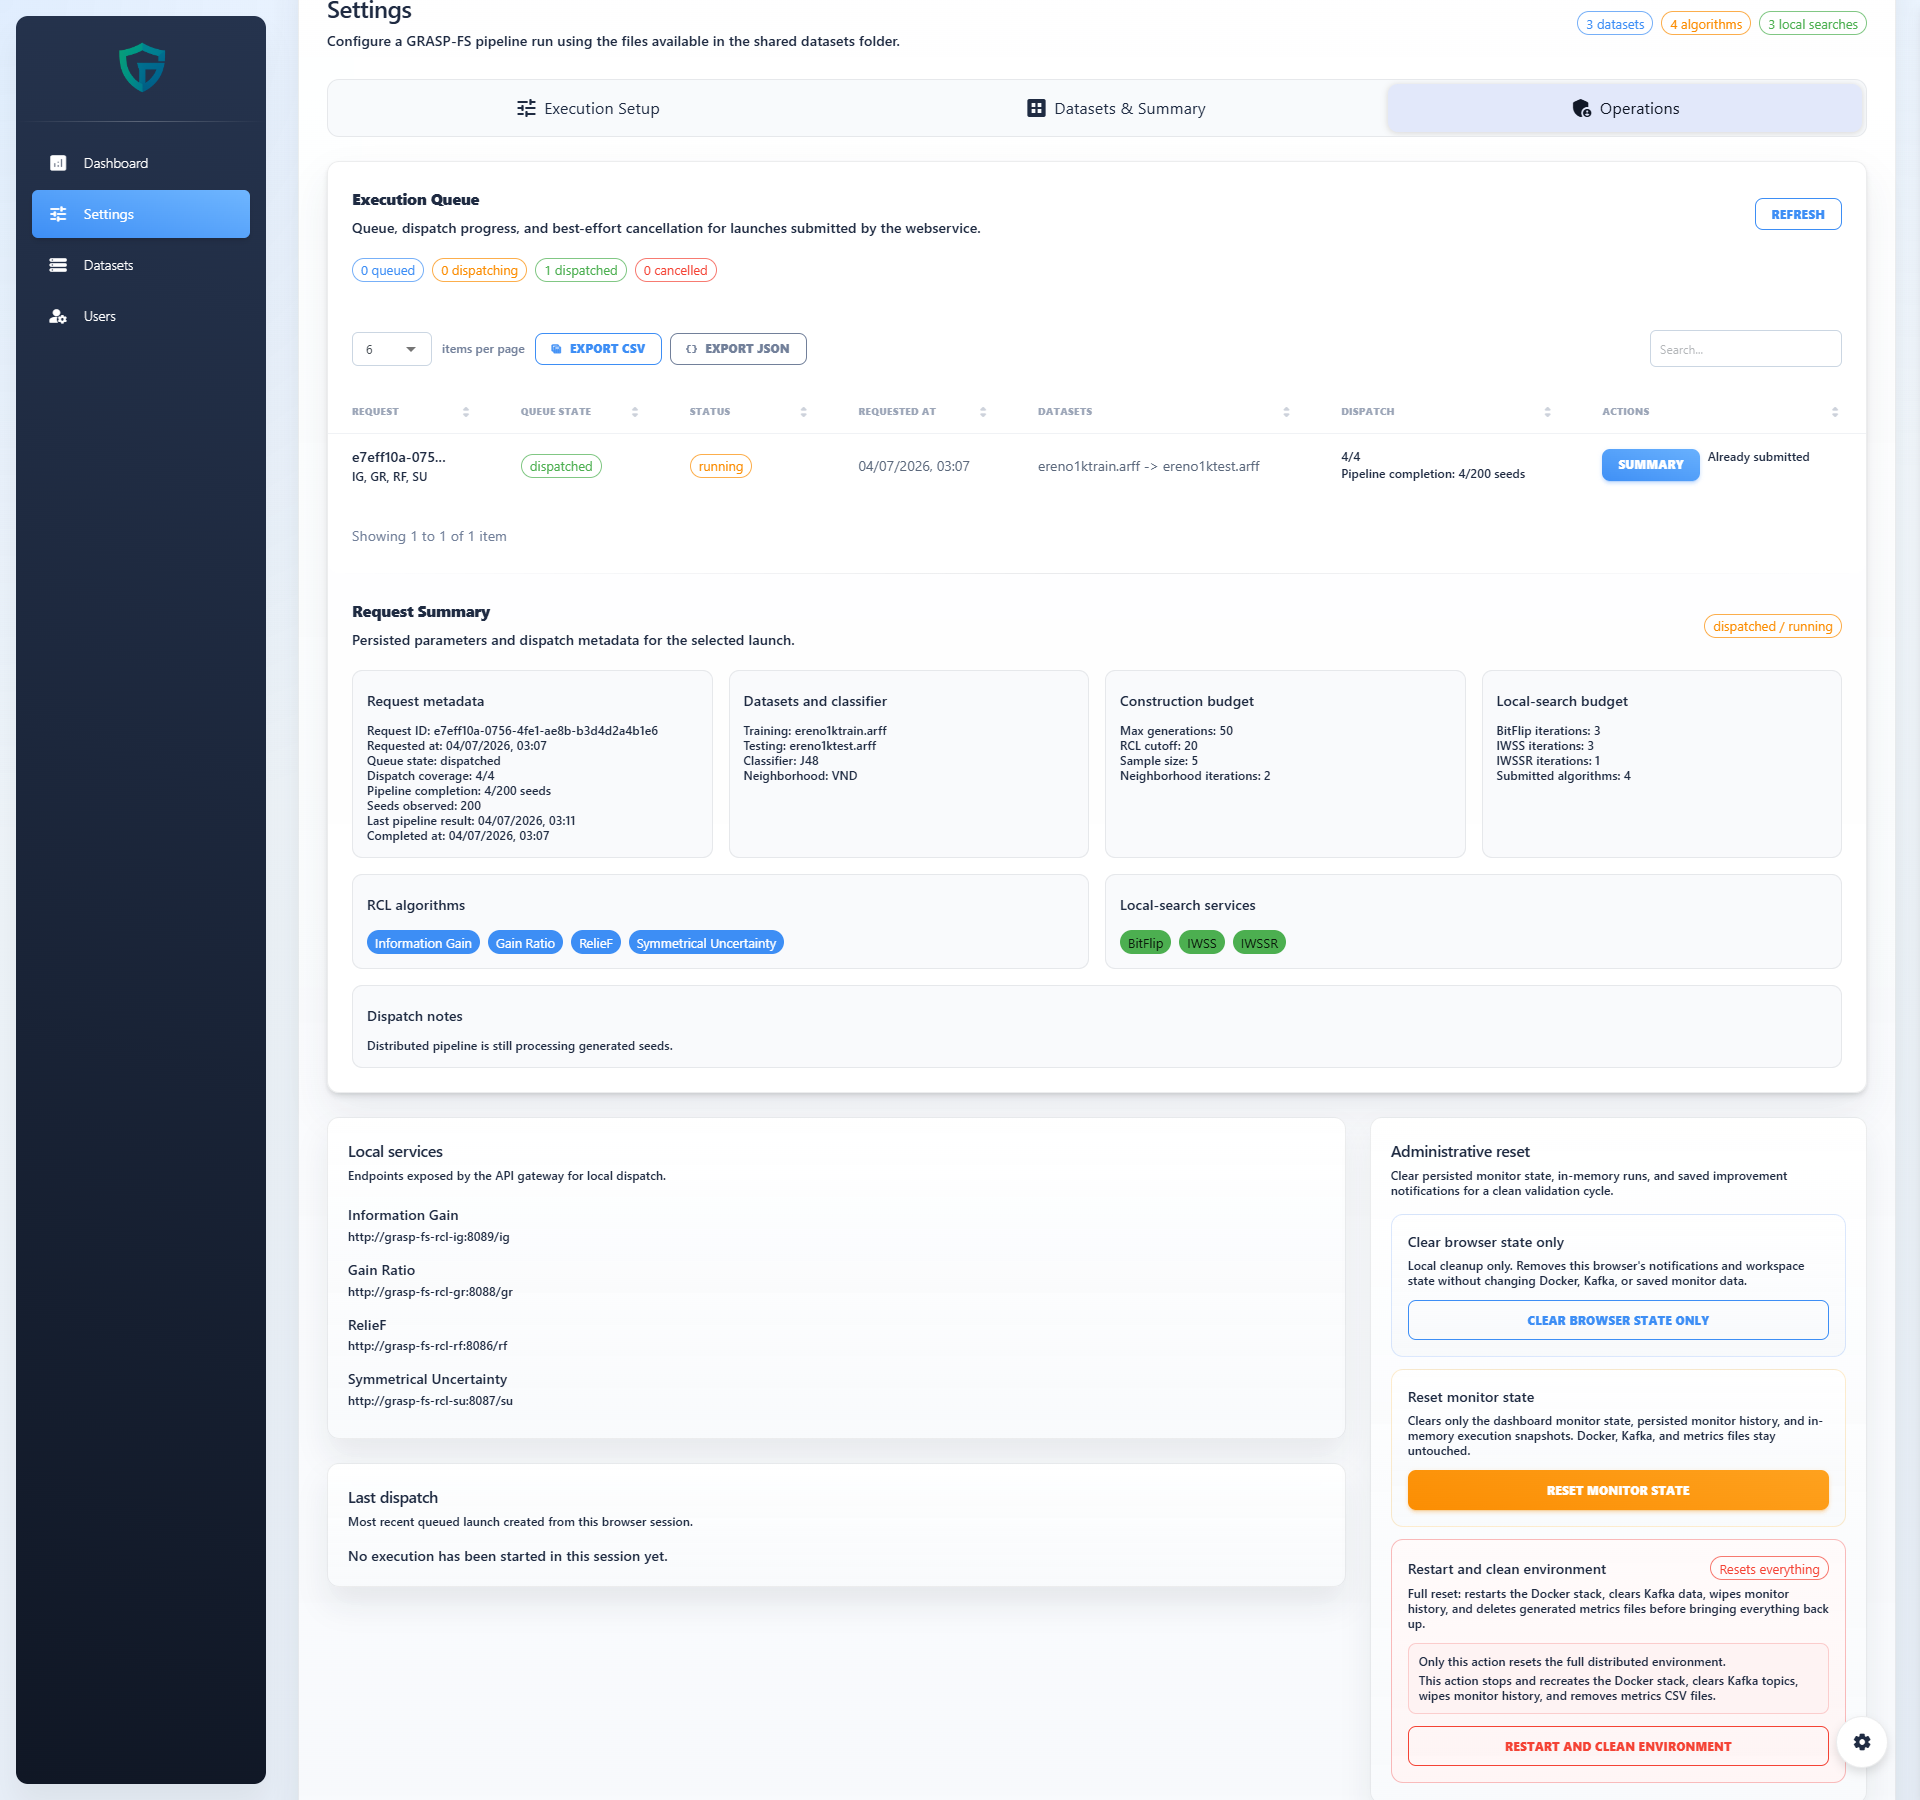
\includegraphics[width=\linewidth,height=0.80\textheight,keepaspectratio]{fig/front/17-settings-operations.png}
  \caption{Operations settings.}
  \label{fig:app-front-settings-operations}
\end{figure}

\begin{figure}[!htb]
  \centering
  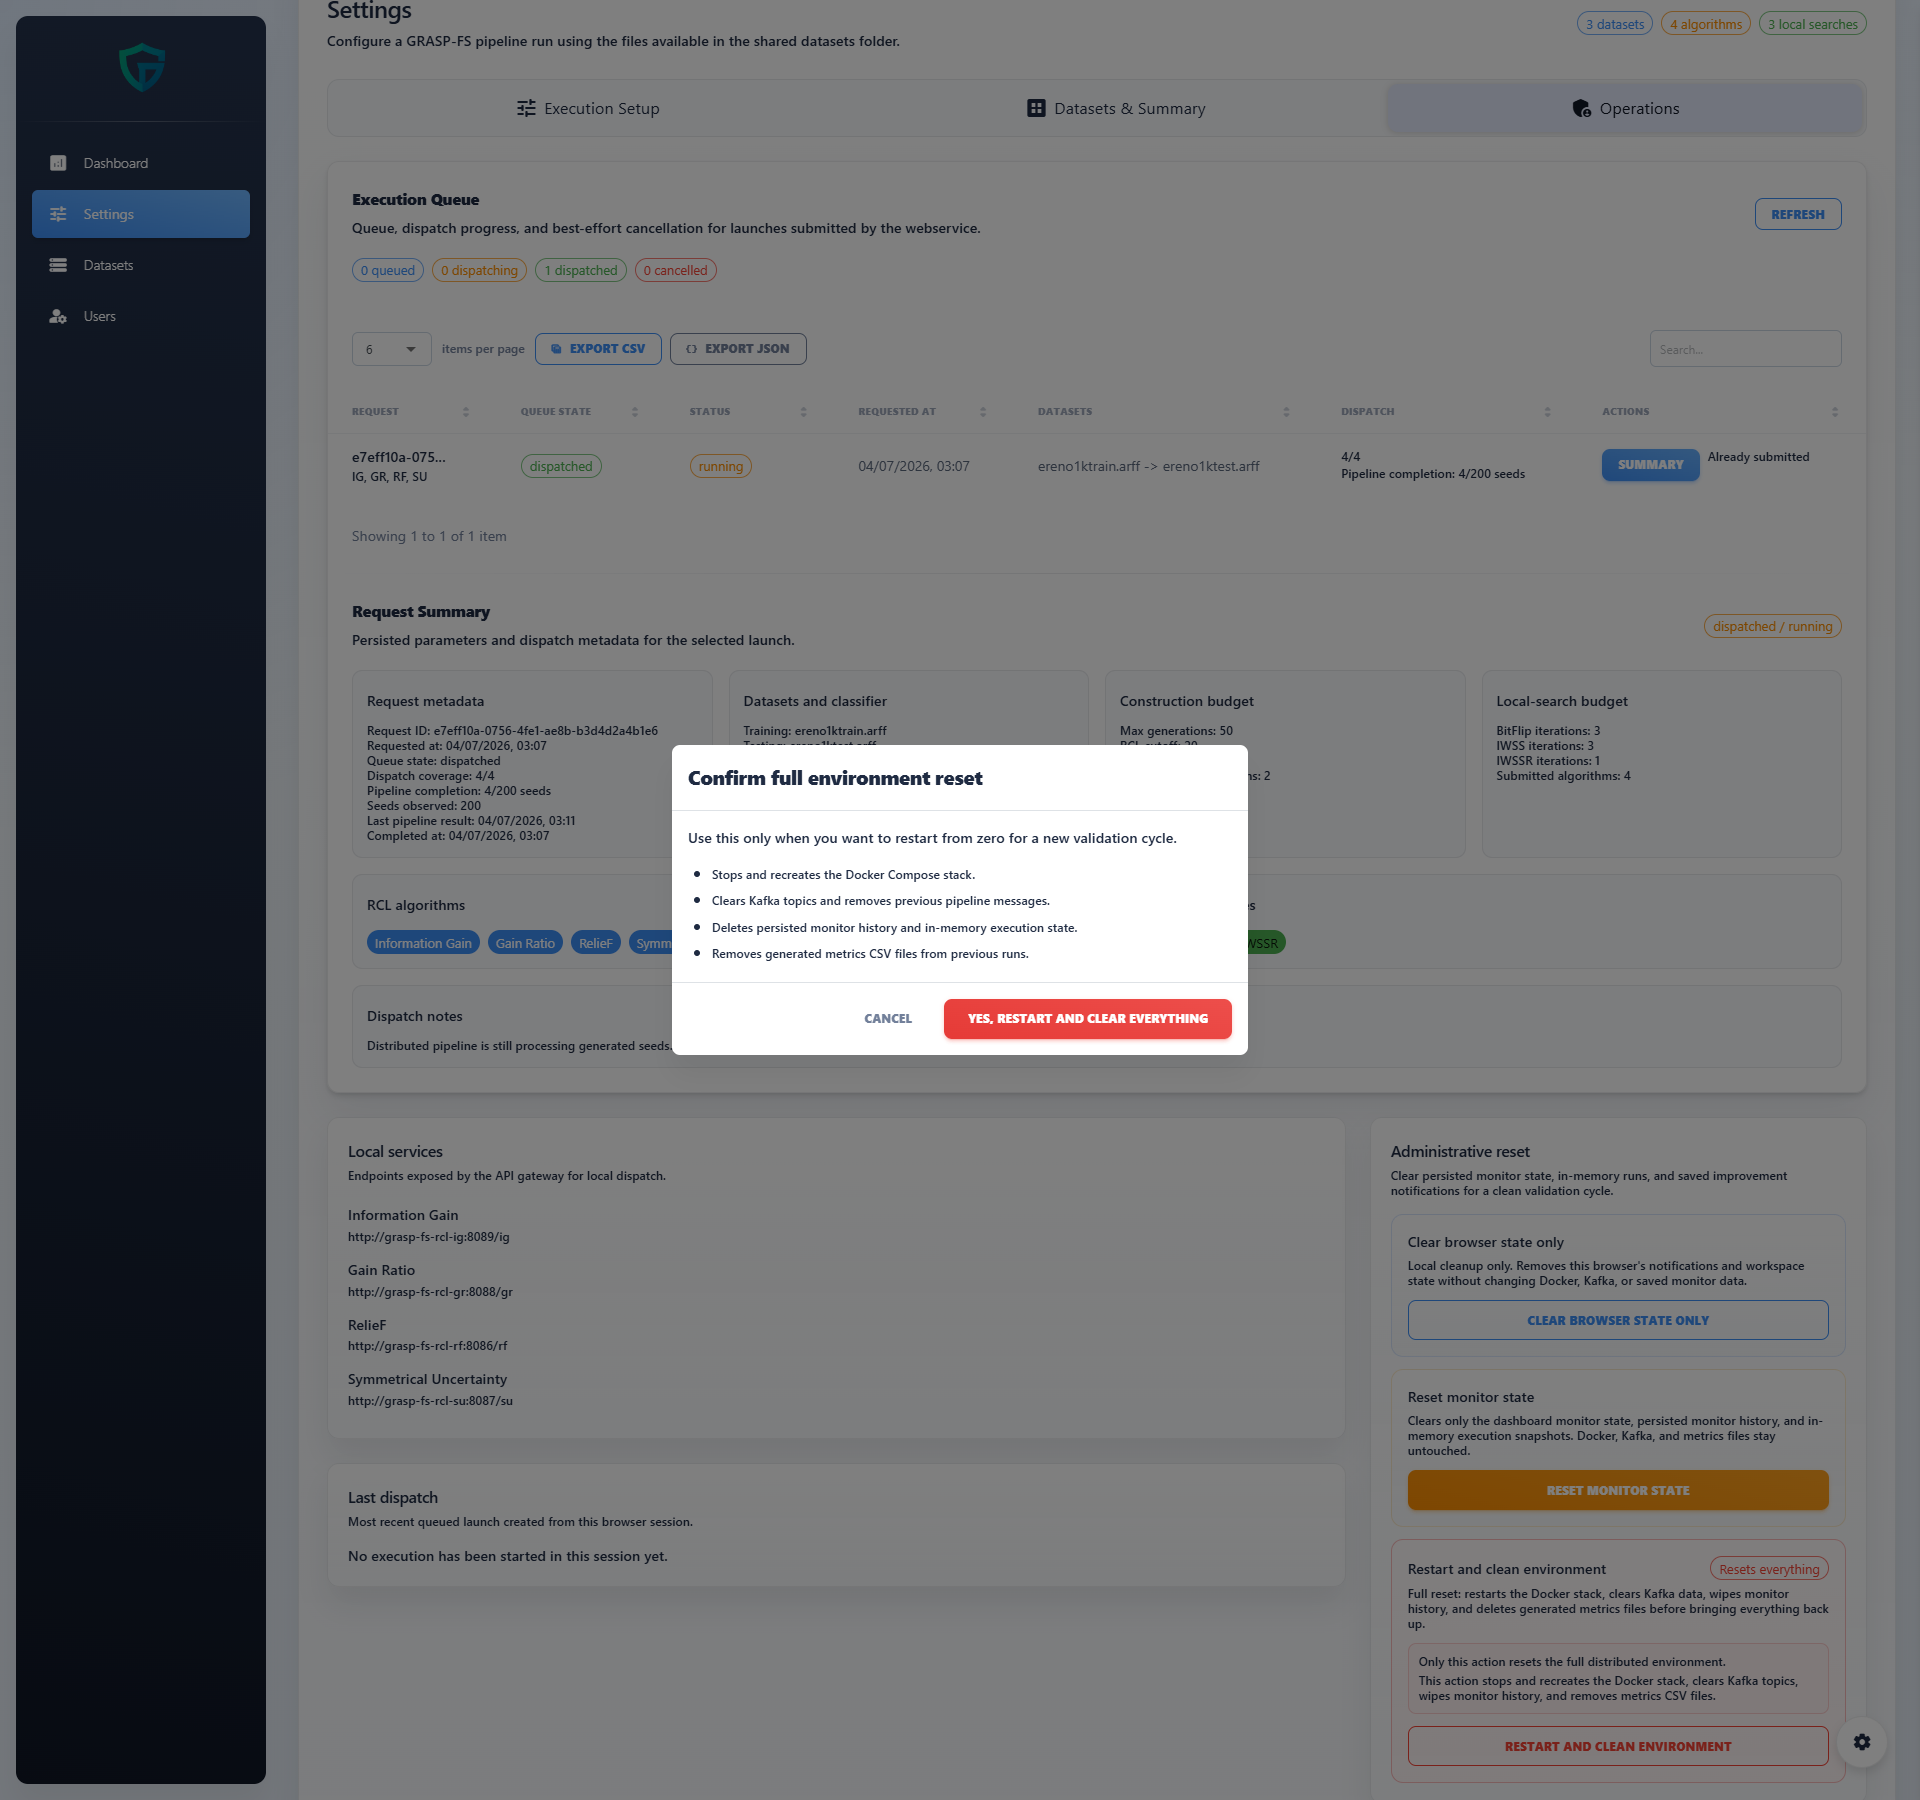
\includegraphics[width=\linewidth,height=0.80\textheight,keepaspectratio]{fig/front/18-settings-full-reset-dialog.png}
  \caption{Full reset dialog.}
  \label{fig:app-front-settings-reset}
\end{figure}

\begin{figure}[!htb]
  \centering
  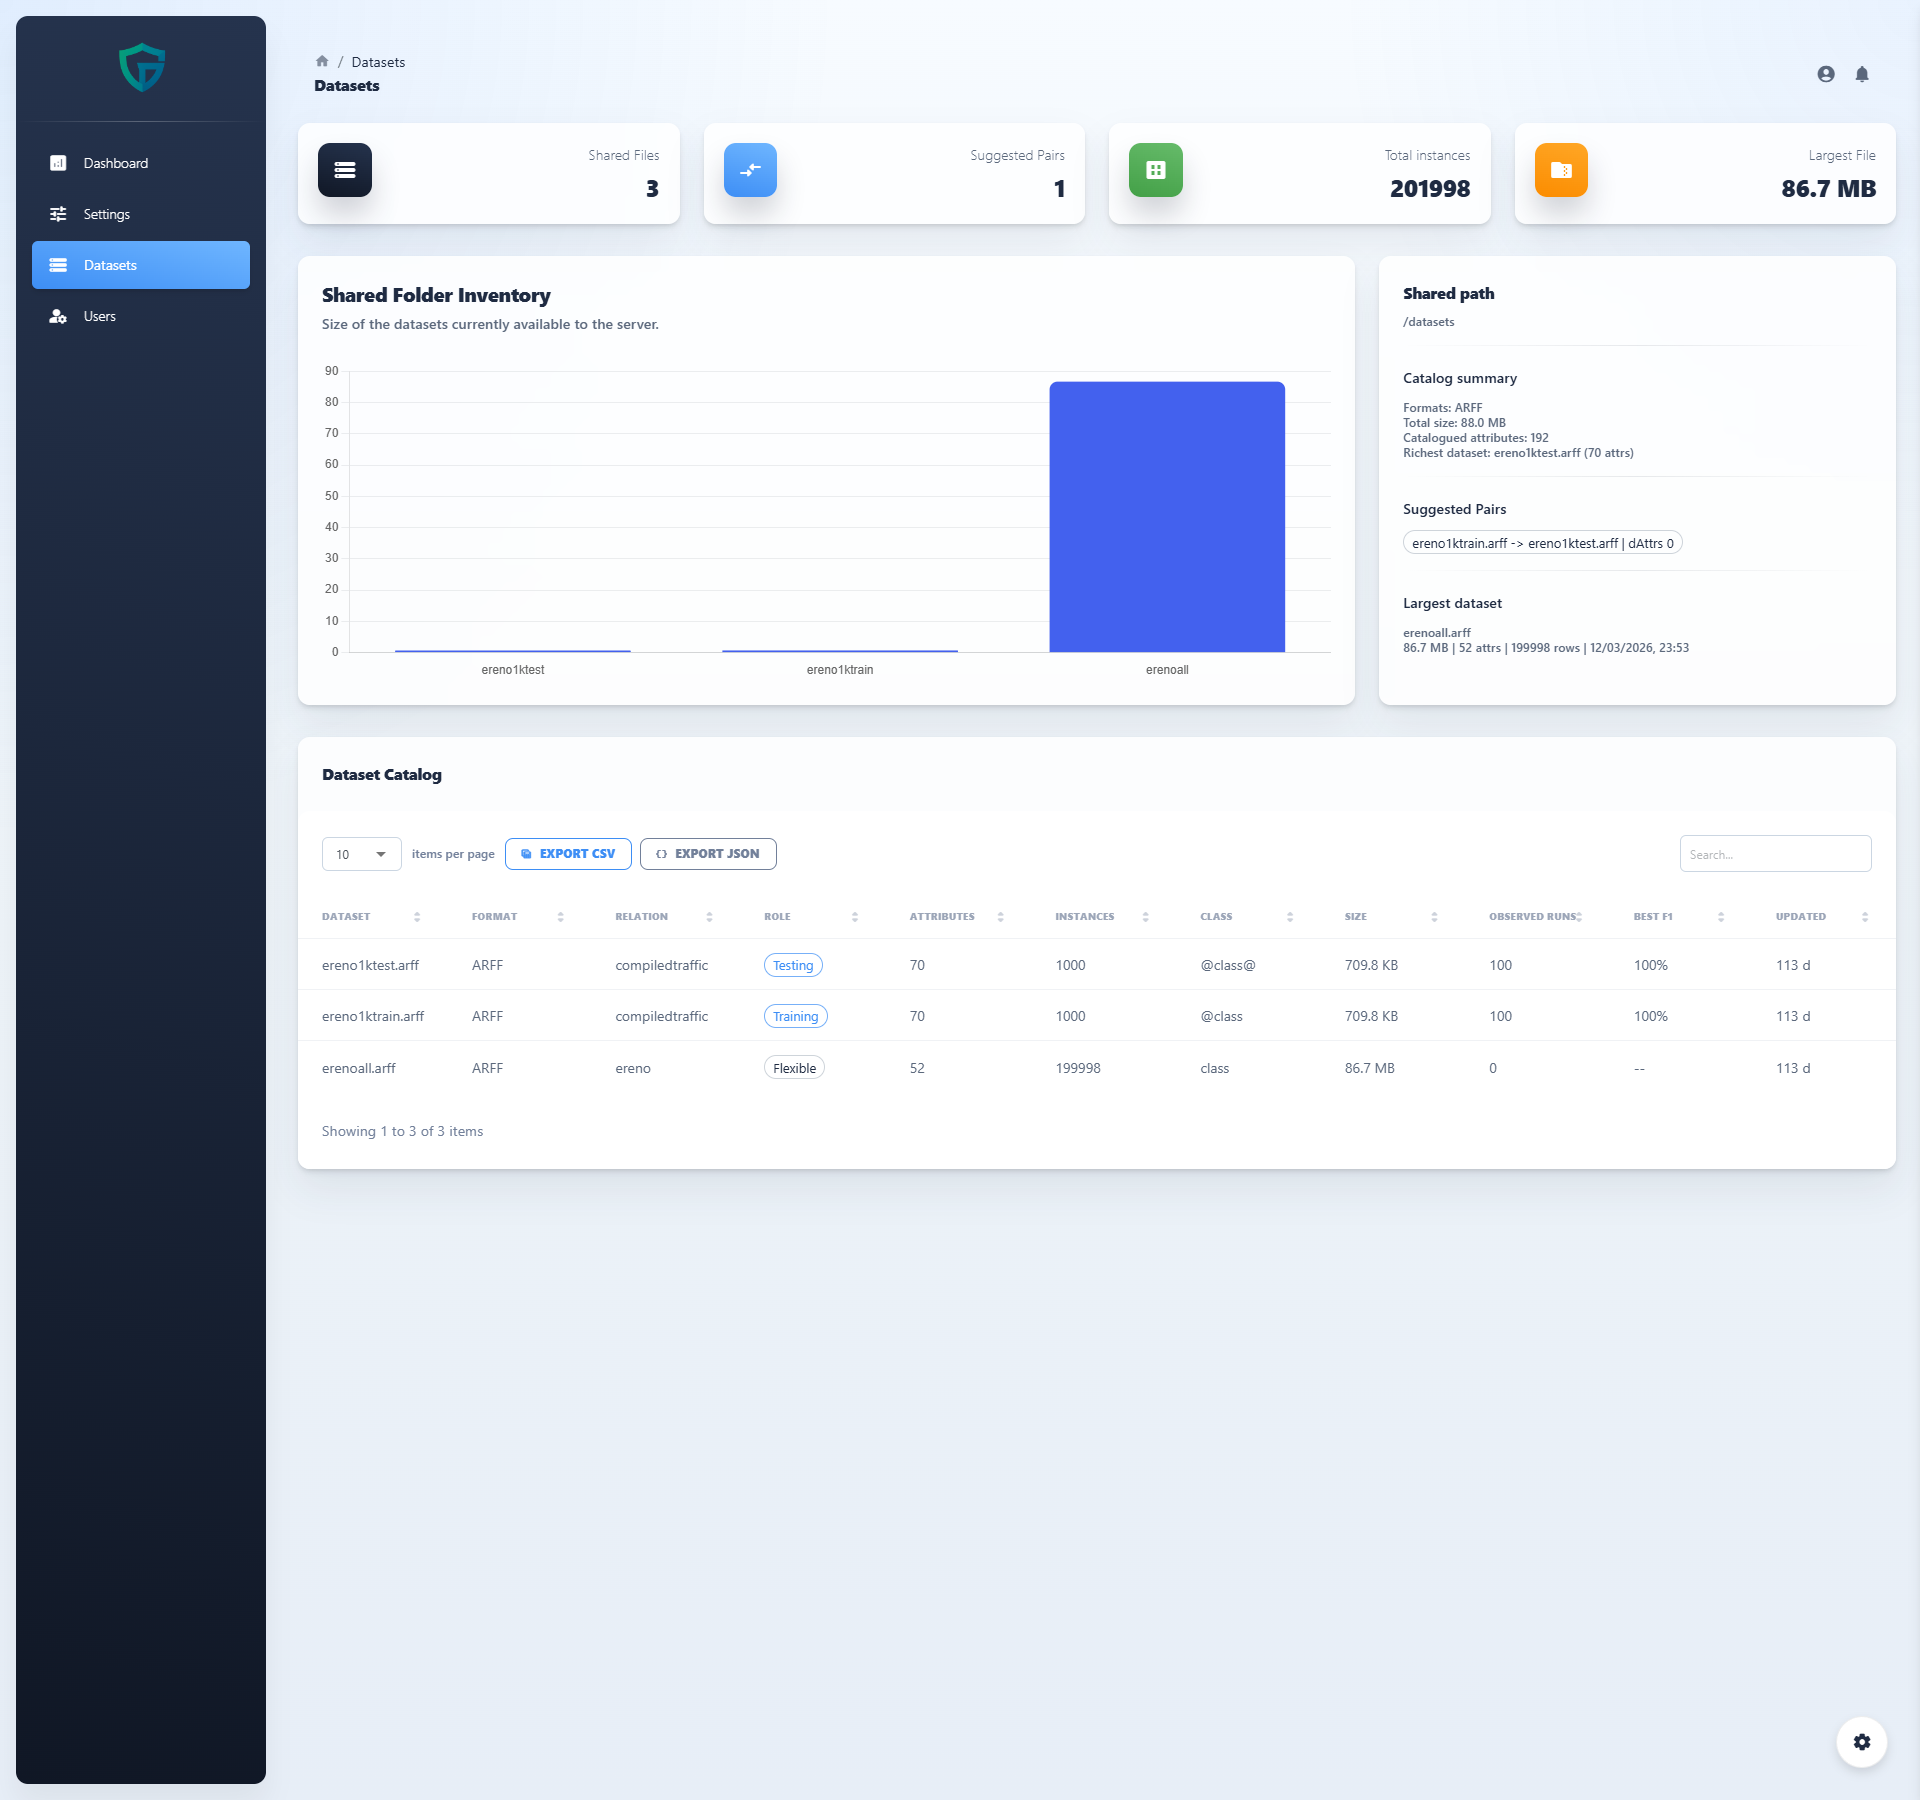
\includegraphics[width=\linewidth,height=0.80\textheight,keepaspectratio]{fig/front/19-datasets.png}
  \caption{Dataset list.}
  \label{fig:app-front-datasets}
\end{figure}

\begin{figure}[!htb]
  \centering
  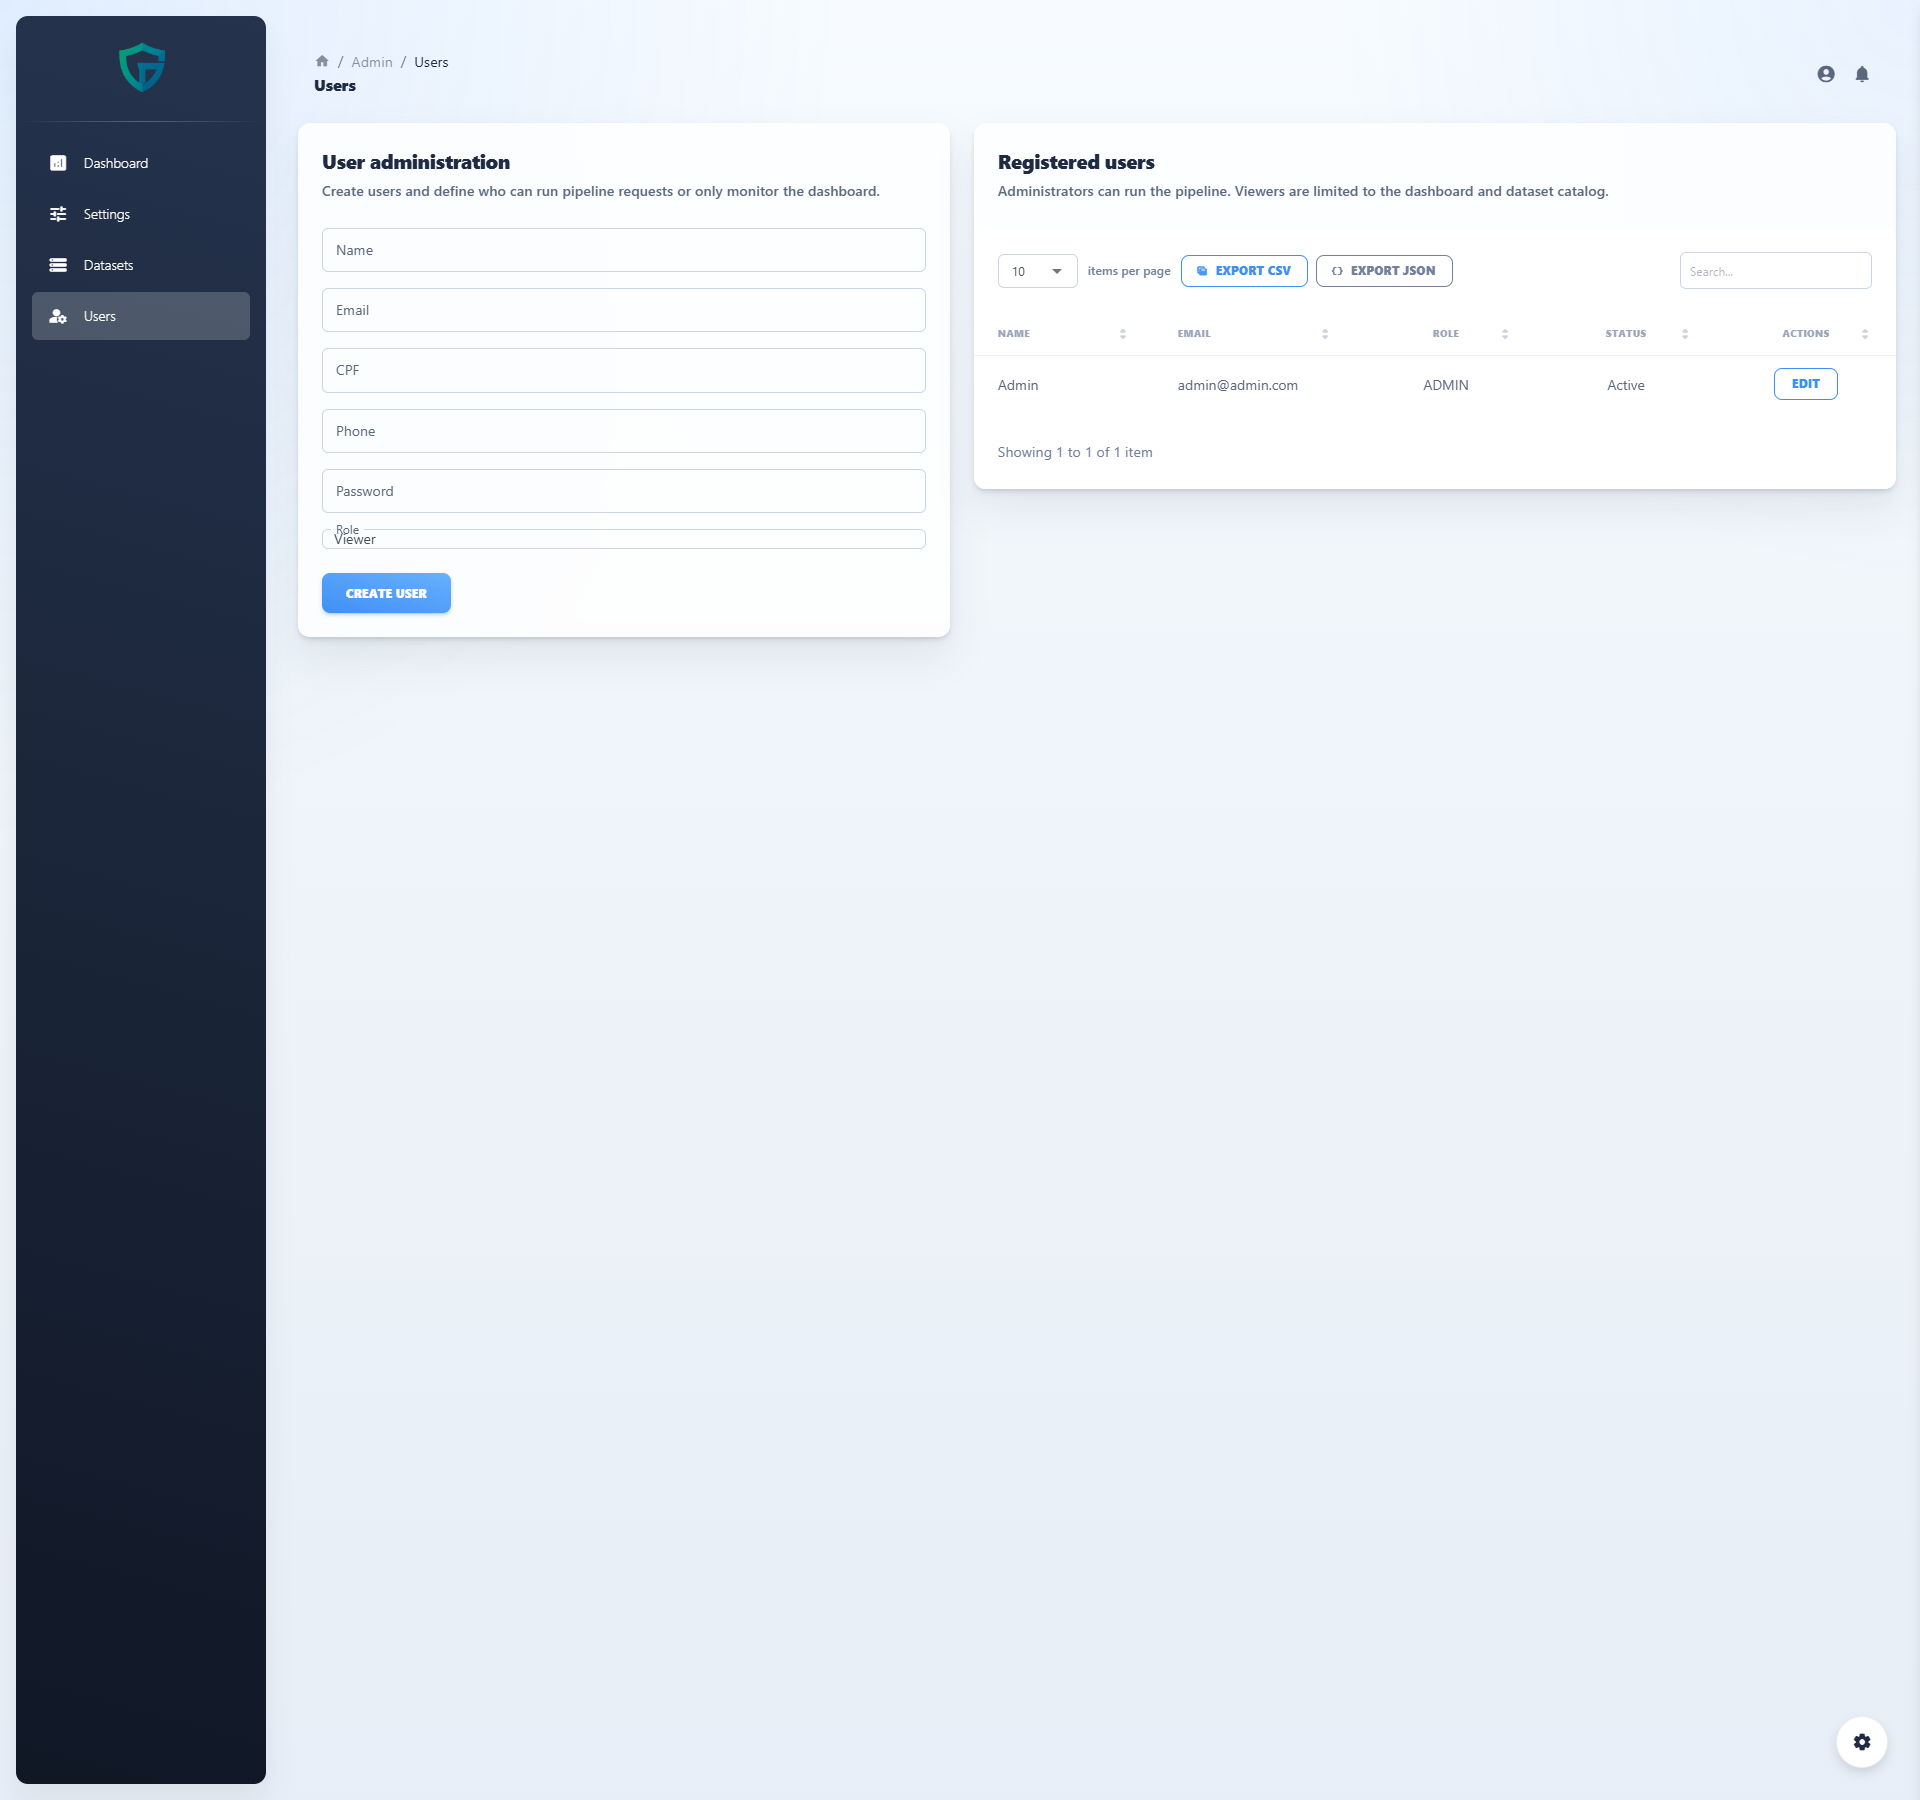
\includegraphics[width=\linewidth,height=0.80\textheight,keepaspectratio]{fig/front/20-users-list.png}
  \caption{User list.}
  \label{fig:app-front-users-list}
\end{figure}

\begin{figure}[!htb]
  \centering
  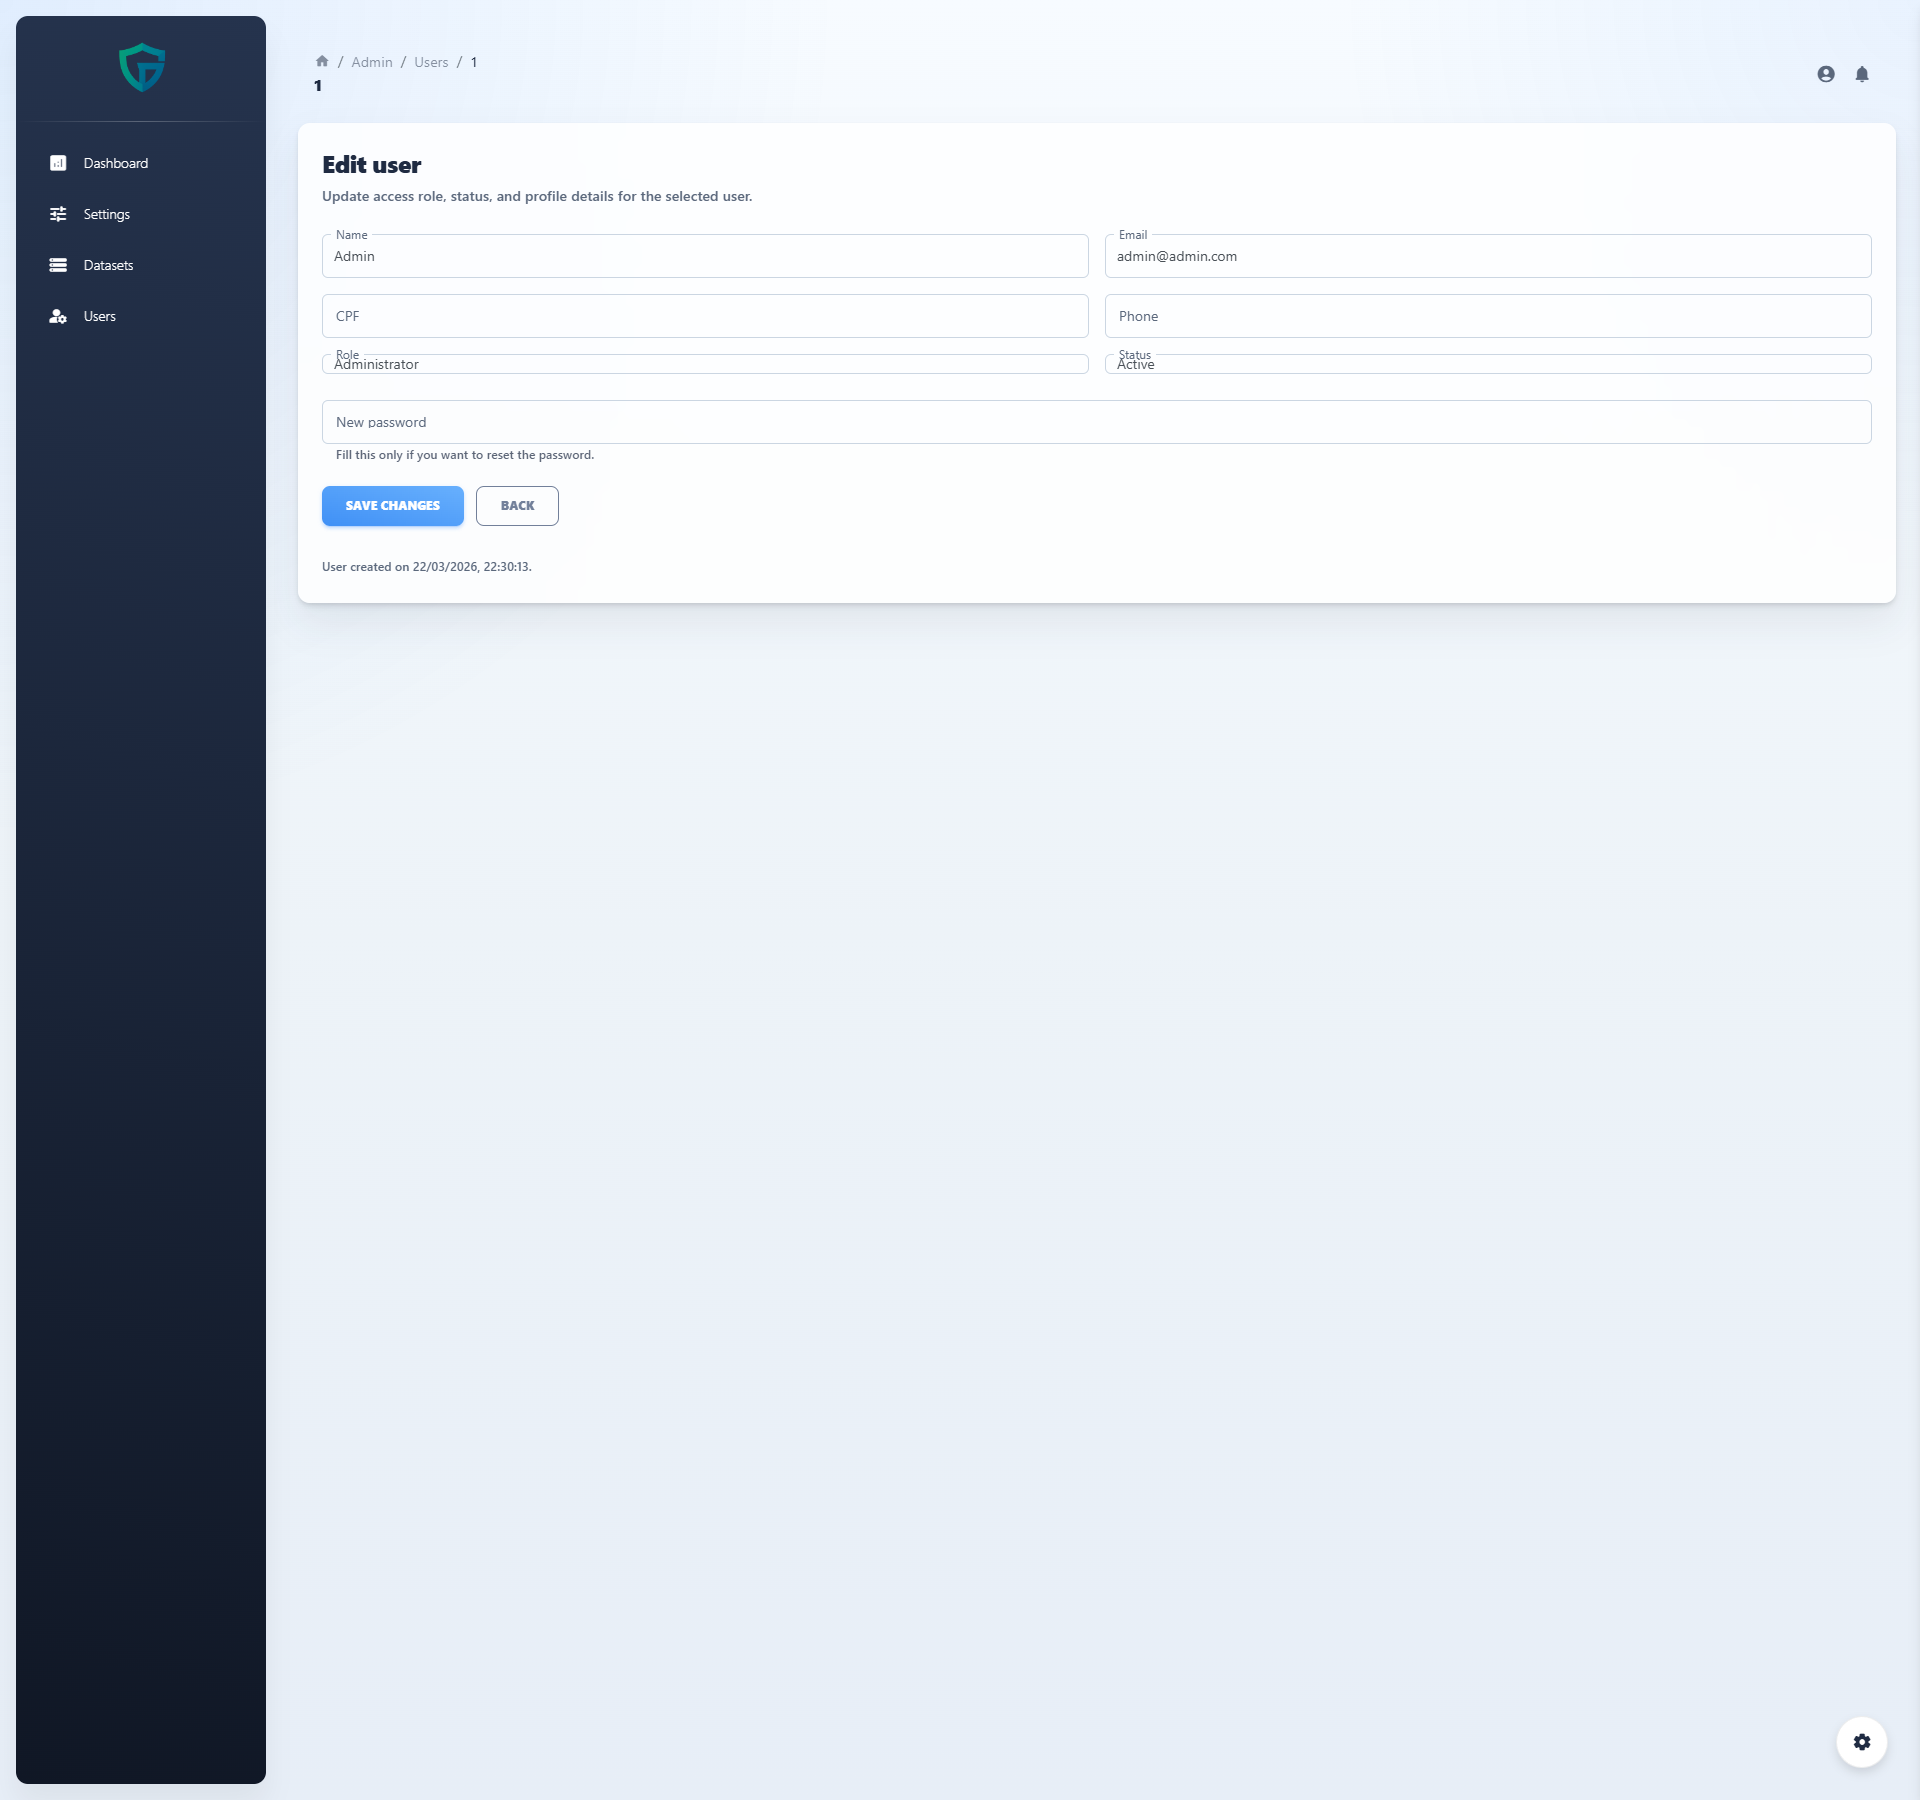
\includegraphics[width=\linewidth,height=0.80\textheight,keepaspectratio]{fig/front/21-user-edit.png}
  \caption{User editing.}
  \label{fig:app-front-user-edit}
\end{figure}

\chapter{Video and Documentation}
\label{app:video-docs}

The platform demo video is included as support material for the defense. Because MP4 files are not always rendered directly by PDF readers, the material is provided by link and is also kept in the project's figure directory.
The poster helps identify the video content when the PDF is opened in a viewer that does not embed media.
Figures~\ref{fig:app-front-video-poster} and~\ref{fig:app-backend-swagger} complete the support material with the demo and API documentation.

\begin{figure}[!htb]
  \centering
  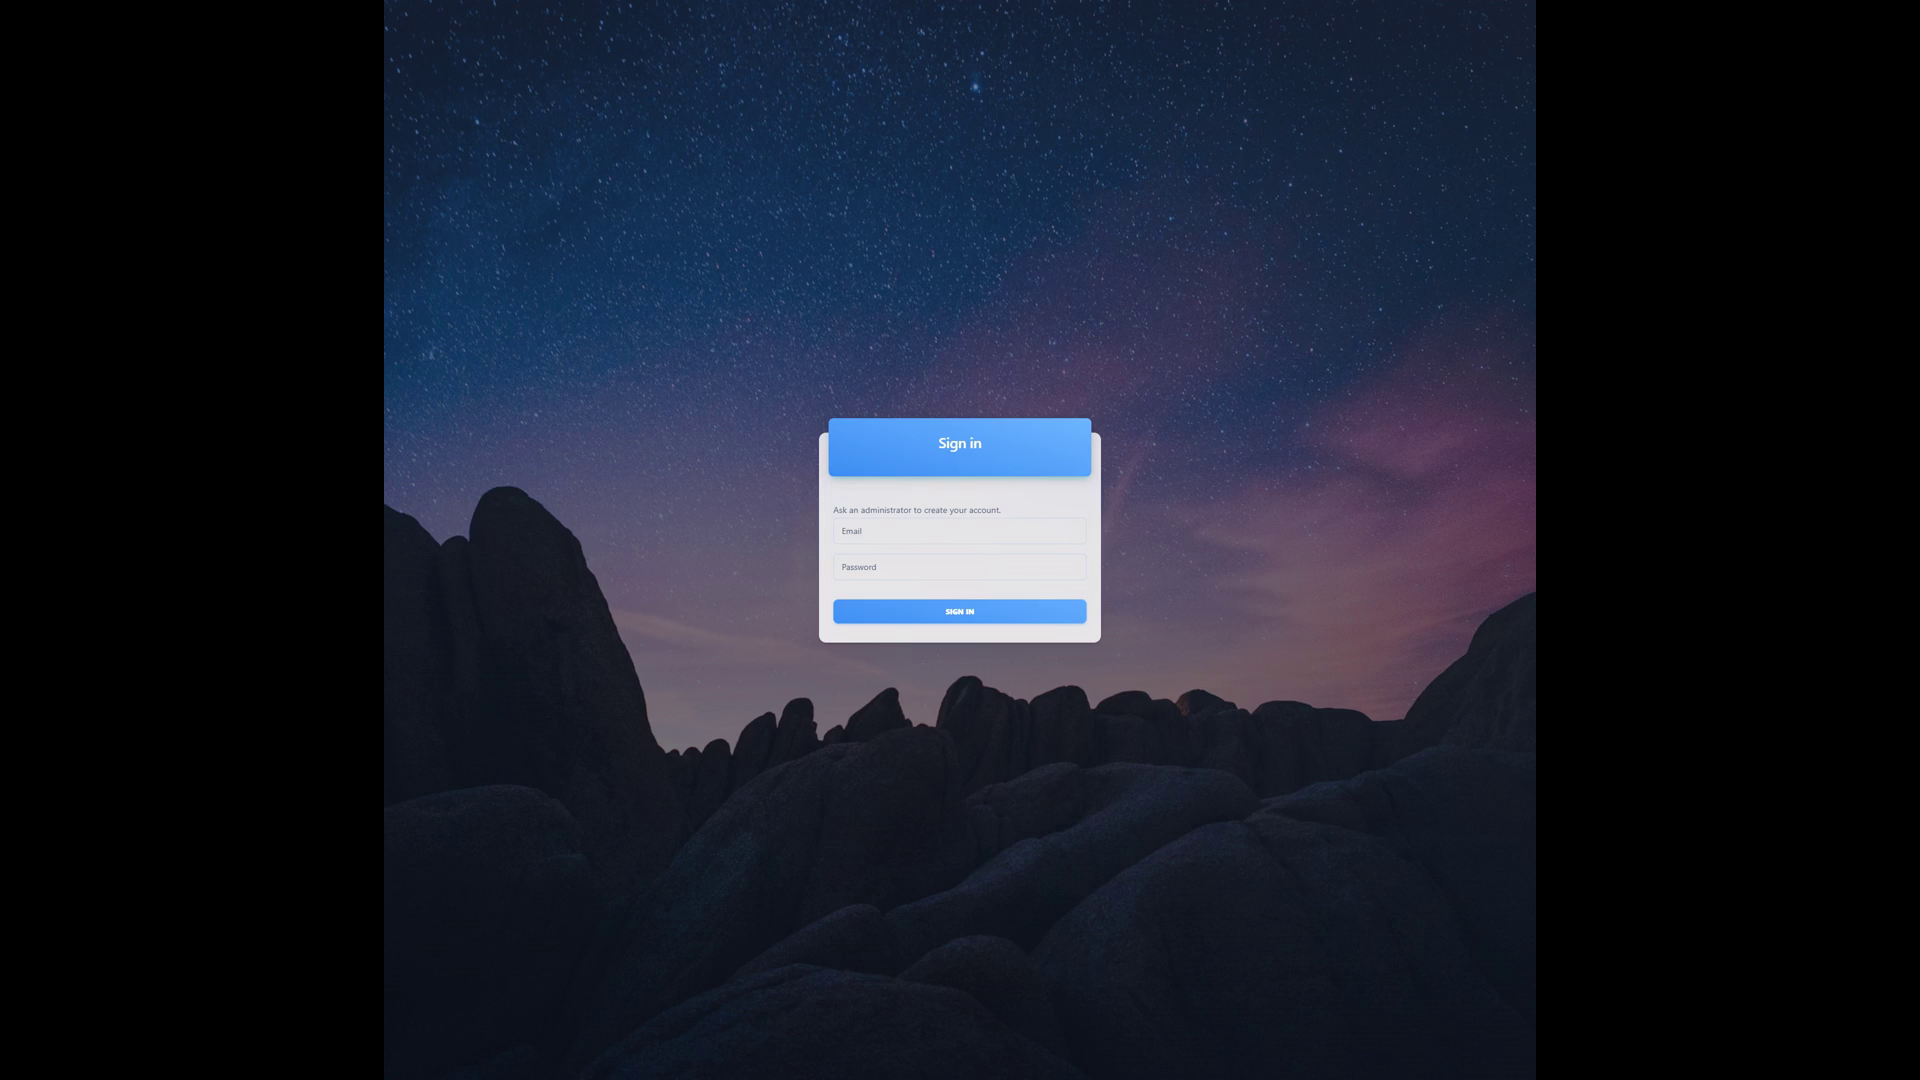
\includegraphics[width=.82\linewidth]{fig/front/site-walkthrough-hd-poster.png}
  \caption{Poster for the platform demo video.}
  \label{fig:app-front-video-poster}
\end{figure}

\noindent\textbf{Demo video:} \url{https://youtu.be/-uqZPaTOjsU}

\vspace{1em}
\noindent The demonstration video should be deposited in a persistent repository or artefact and identified by the version corresponding to this dissertation.

\begin{figure}[!htb]
  \centering
  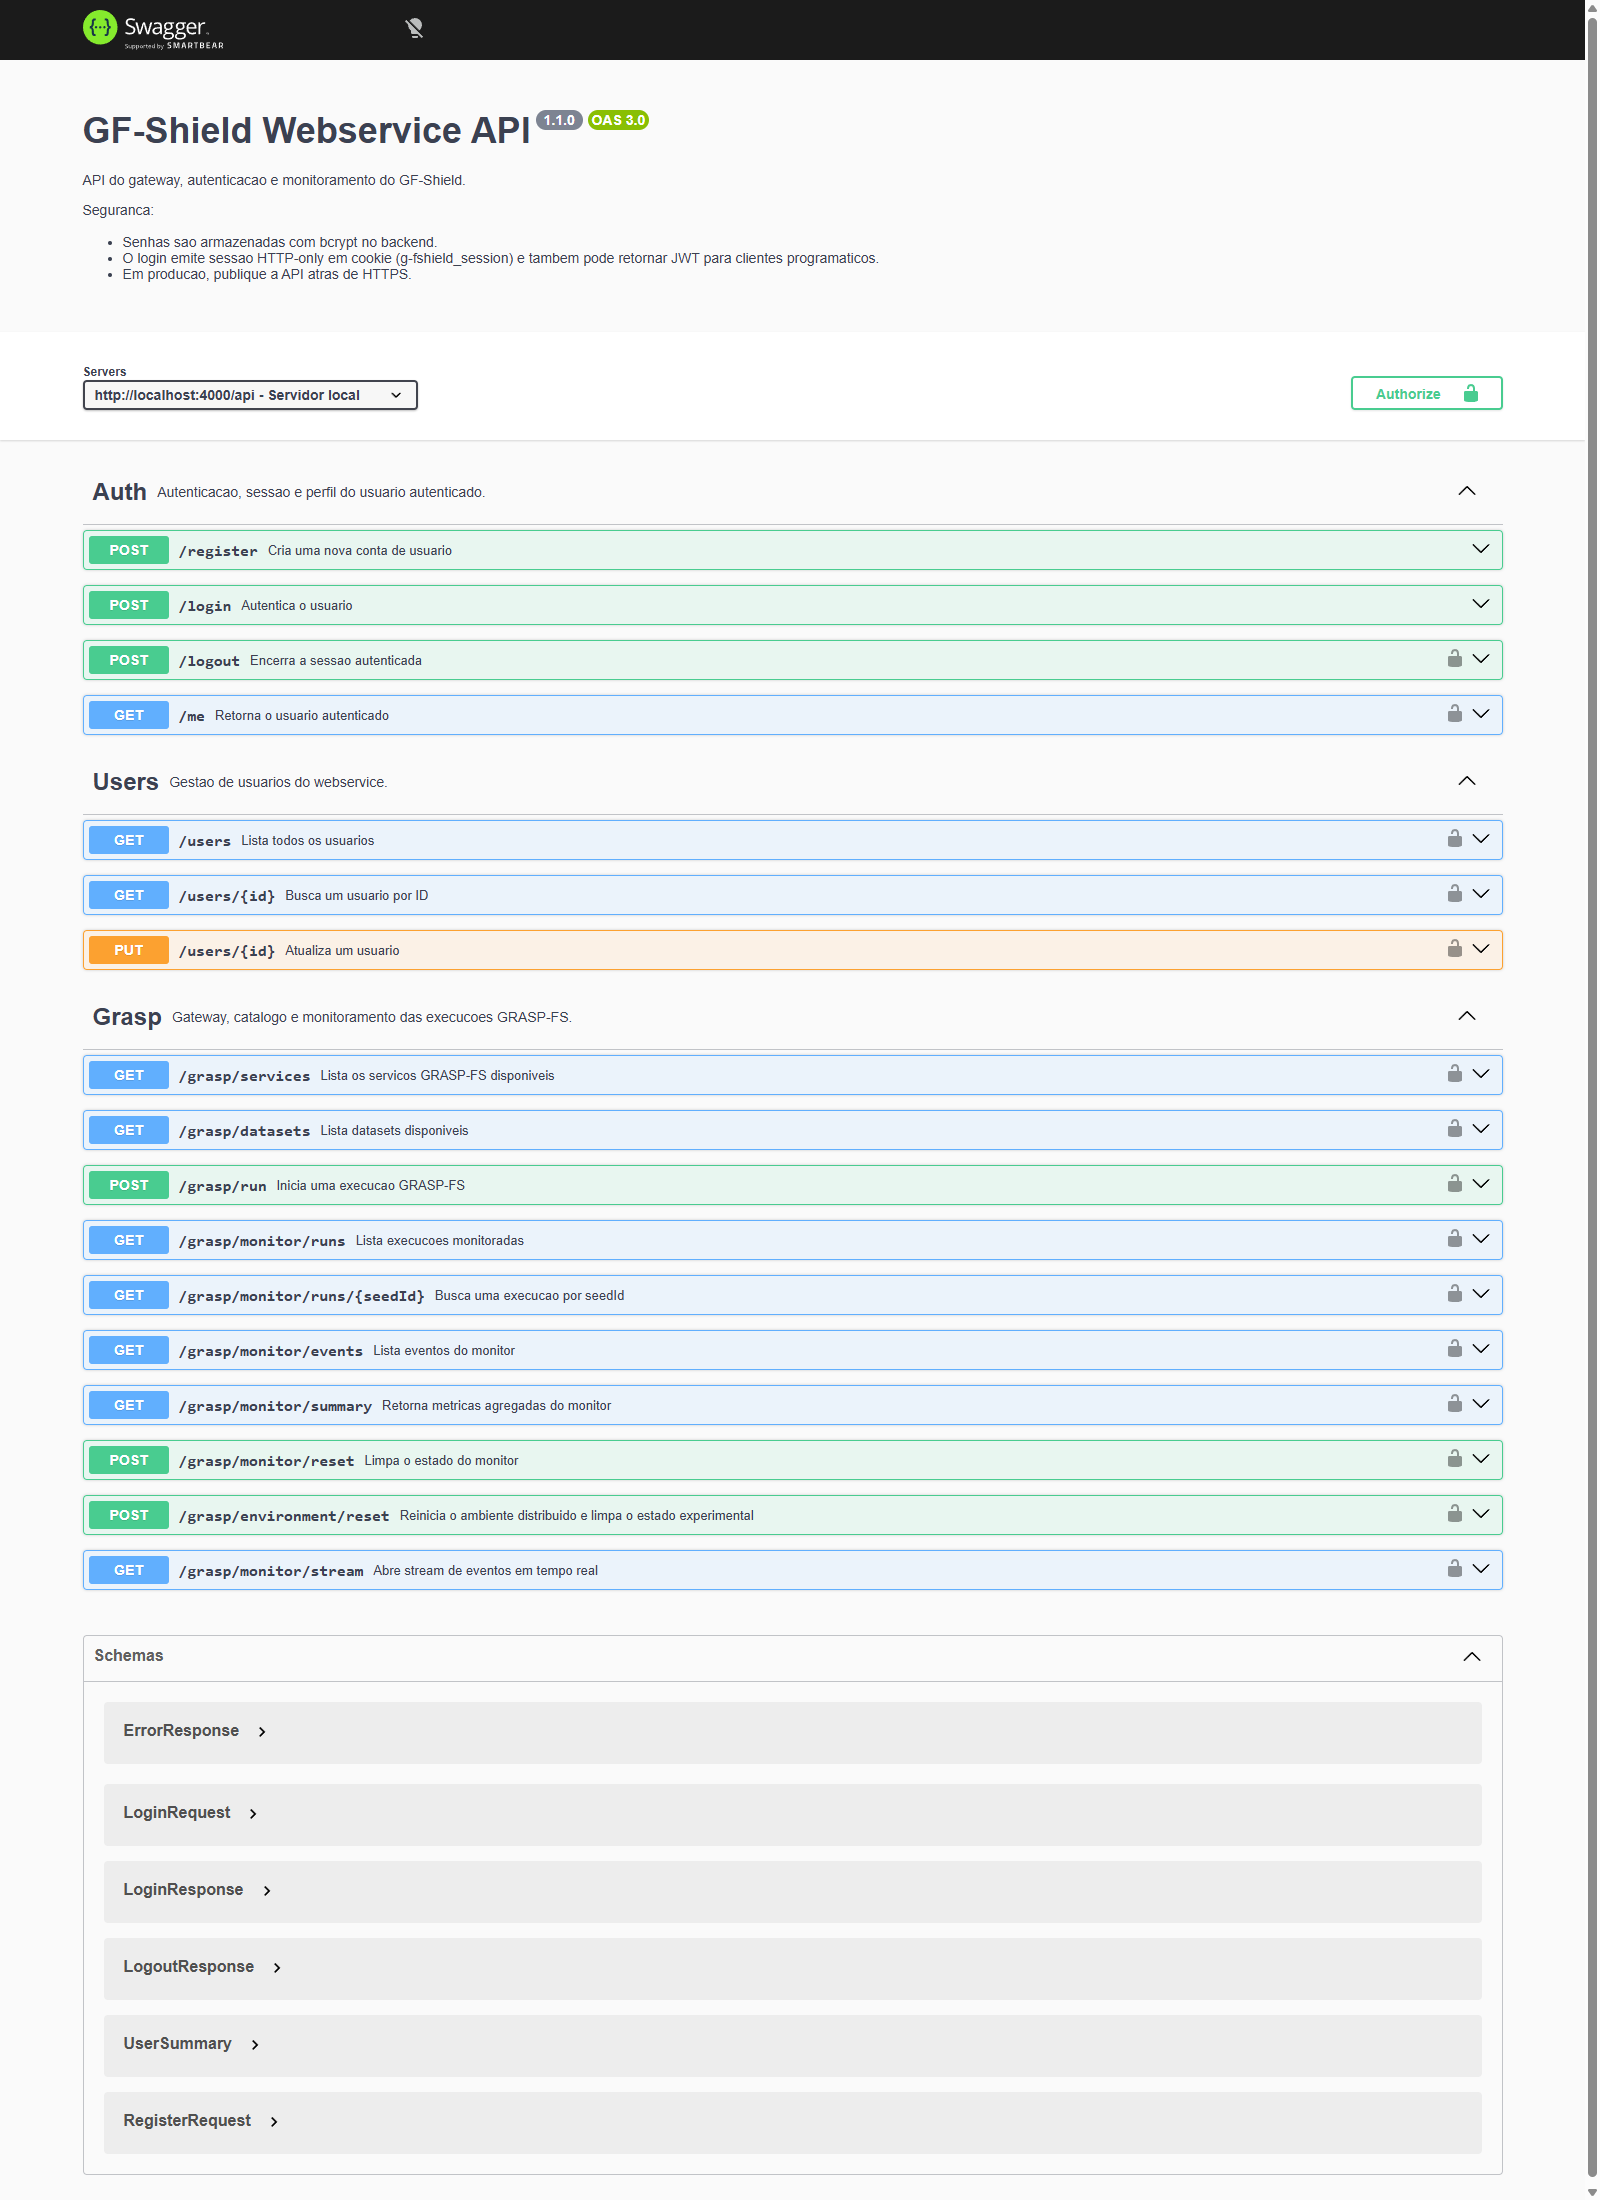
\includegraphics[width=.72\linewidth]{fig/front/swagger-api-docs.png}
  \caption{Swagger documentation of the backend API.}
  \label{fig:app-backend-swagger}
\end{figure}

\chapter{Architecture Diagrams}
\label{app:diagrams}

This appendix gathers the specific diagrams that complement the main architecture discussion.
They connect the development visuals to the screens and operational flows shown in the other sections.
Figures~\ref{fig:app-front-flow},~\ref{fig:app-backend-architecture},~\ref{fig:app-drg-generic}, and~\ref{fig:app-architecture-summary} show the complete architectural chain.

\begin{figure}[!htb]
  \centering
  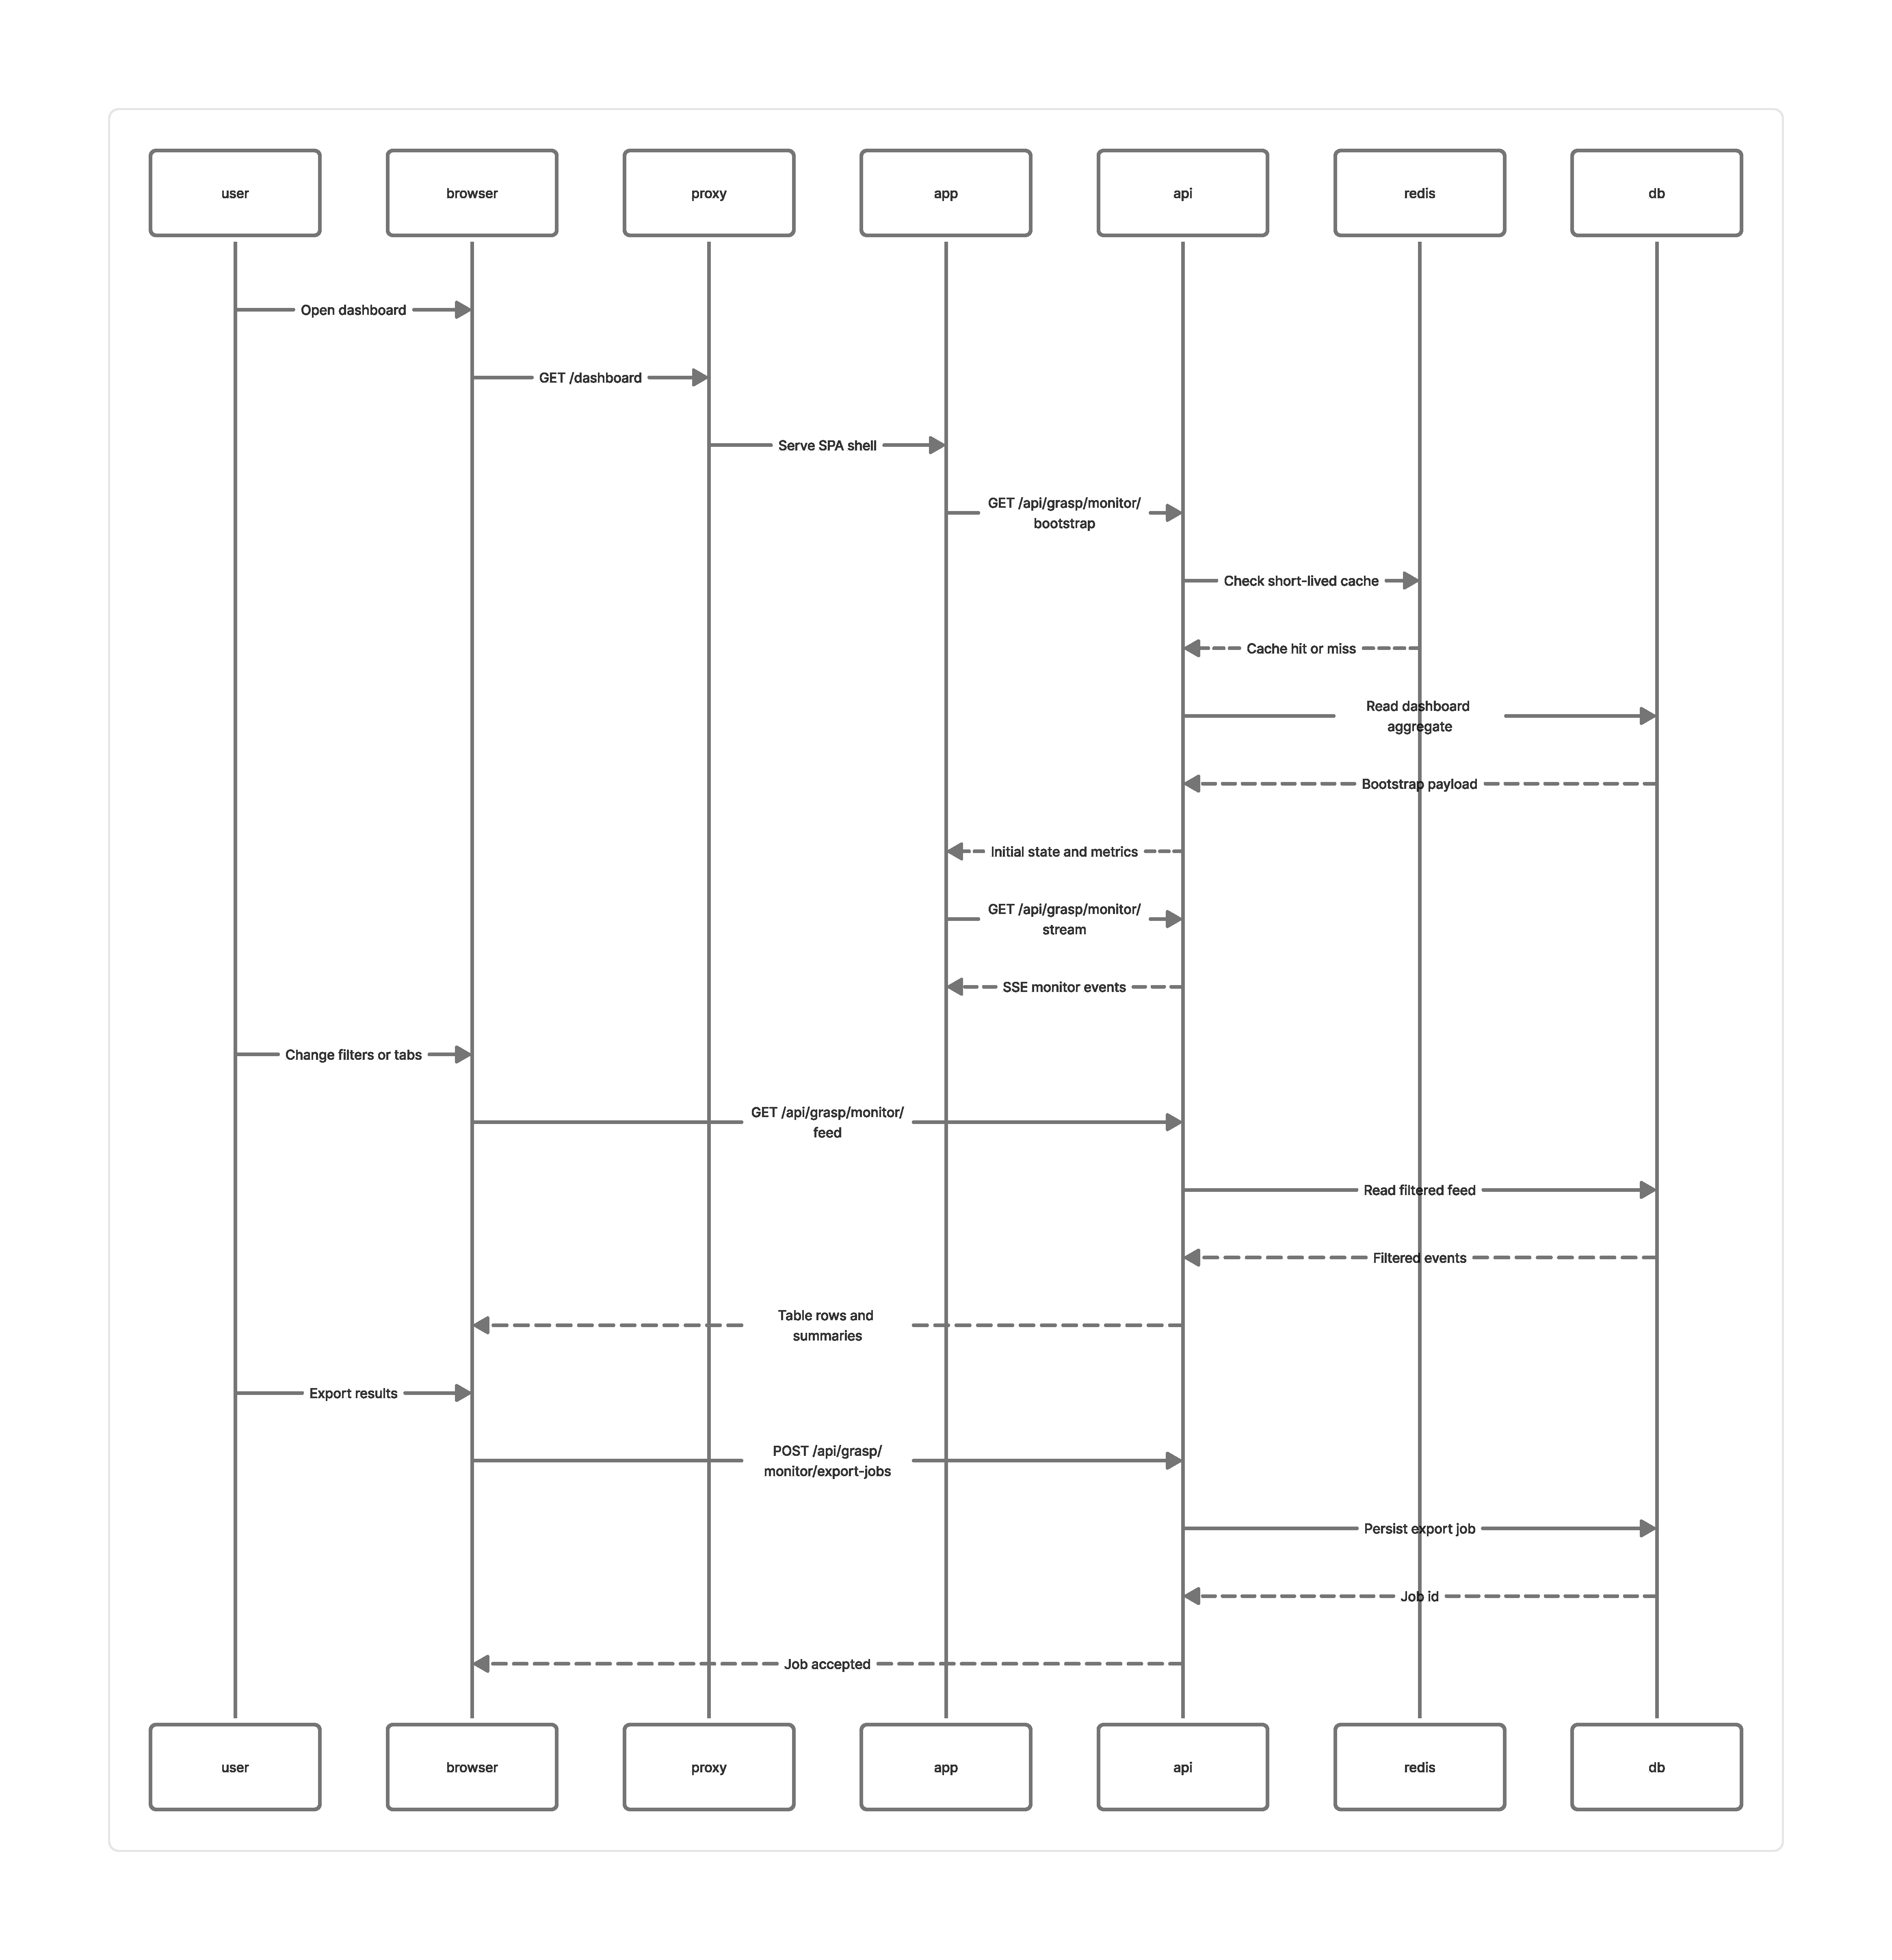
\includegraphics[width=.92\linewidth]{fig/gfshield/gfshield-front-flow.pdf}
  \caption{Frontend flow of the system.}
  \label{fig:app-front-flow}
\end{figure}

\begin{figure}[!htb]
  \centering
  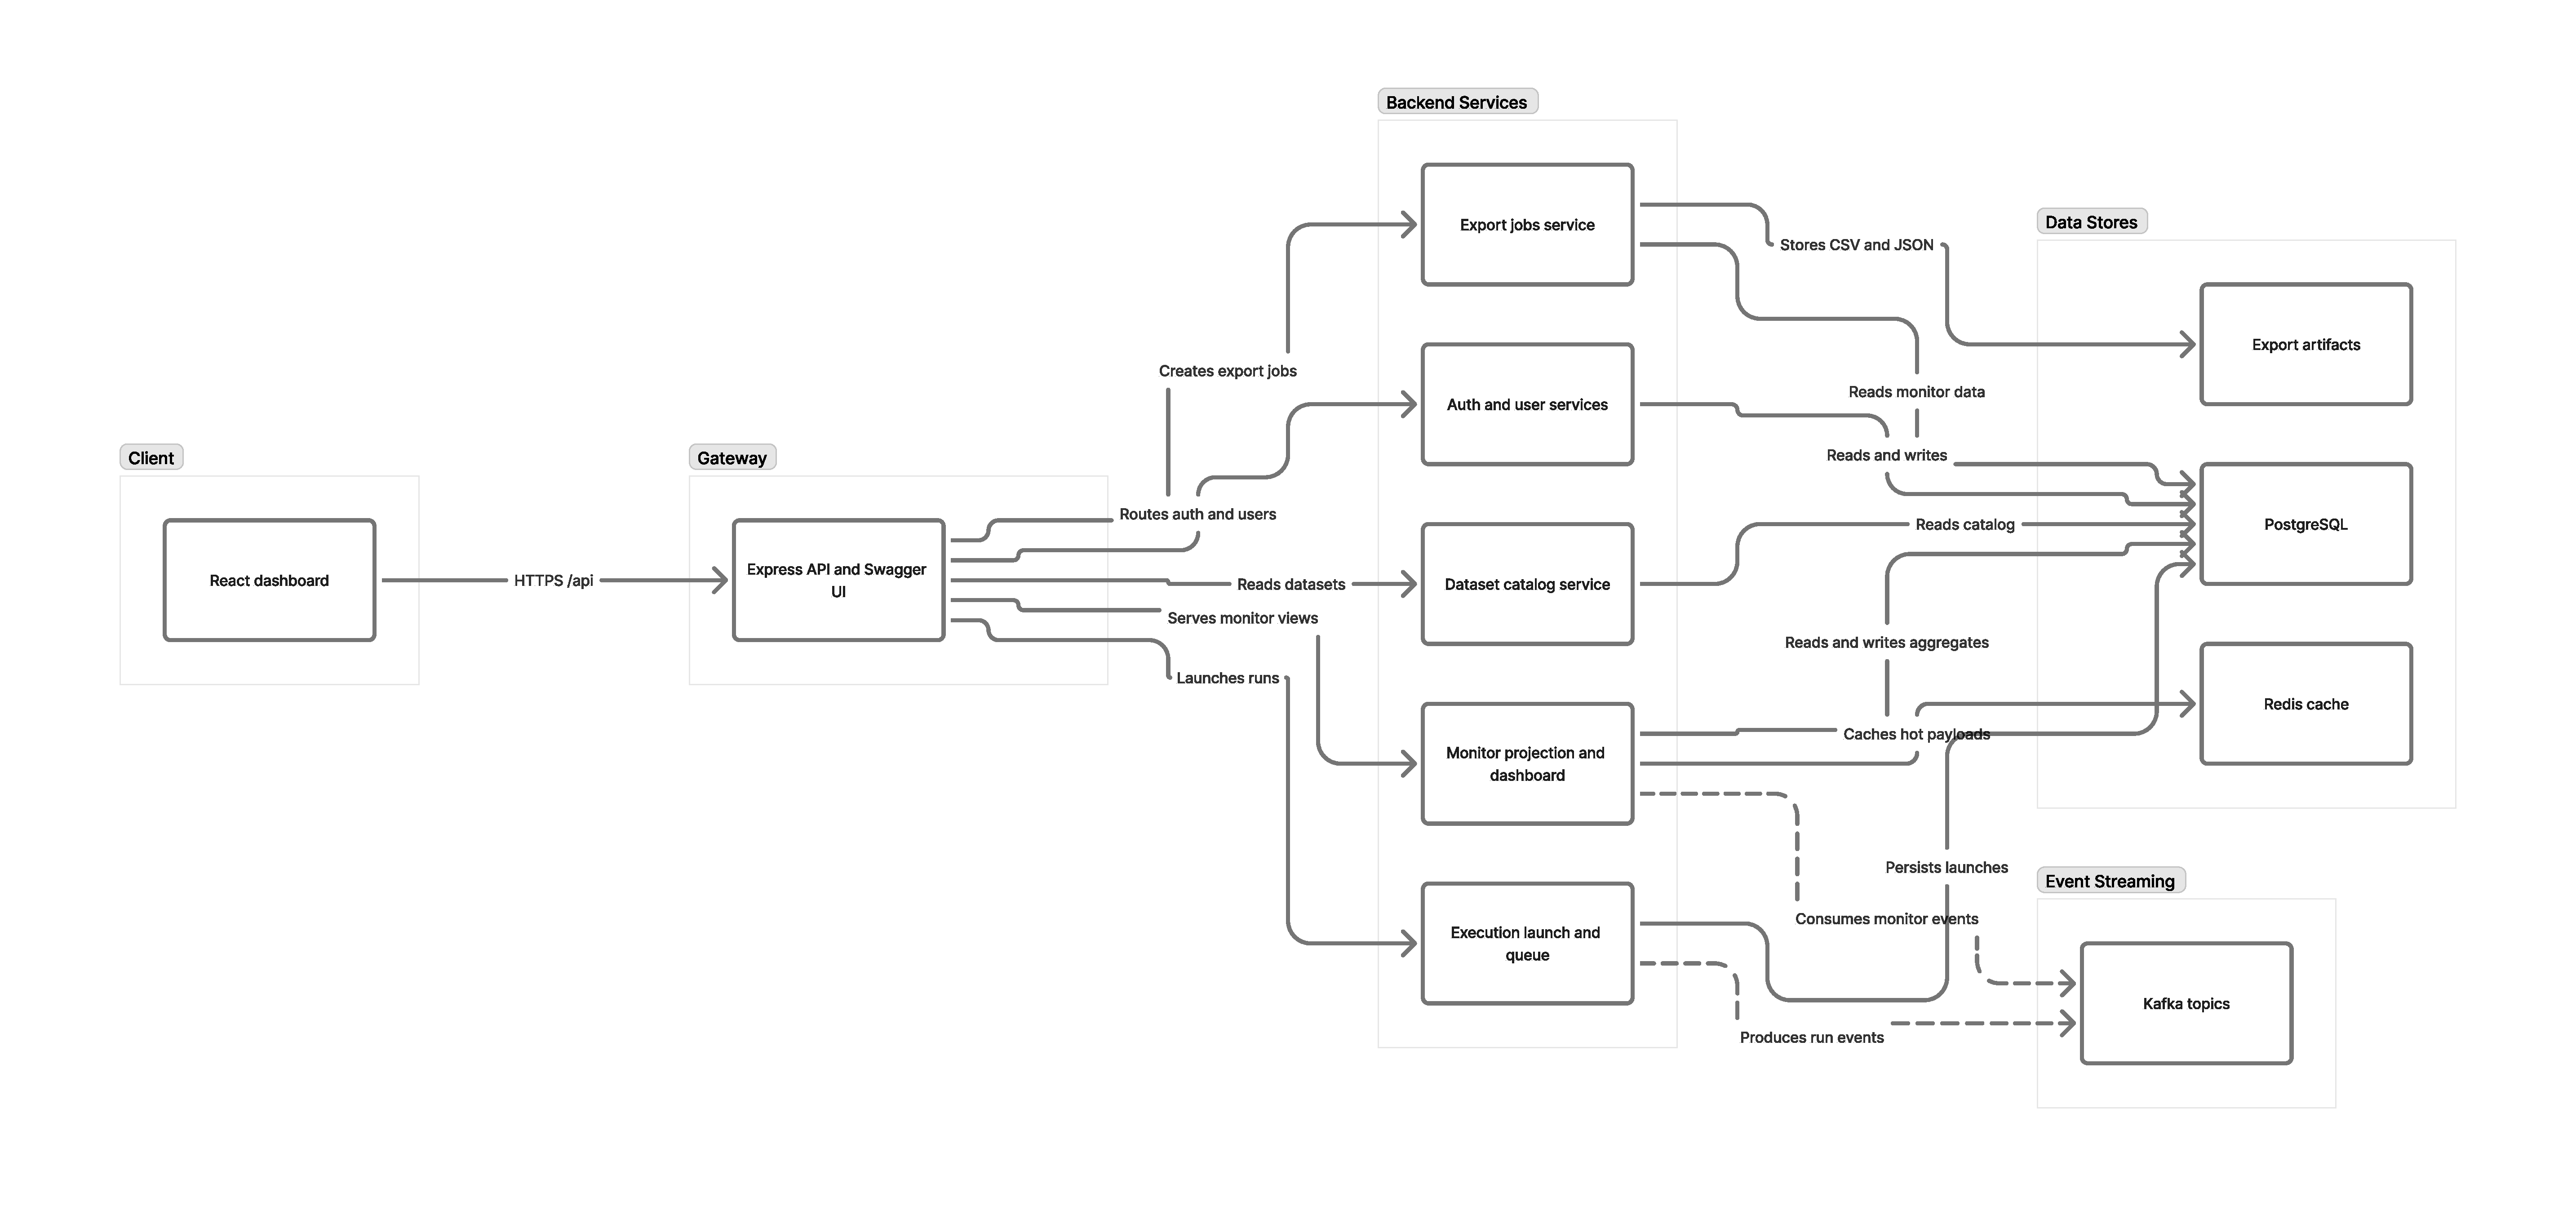
\includegraphics[width=.92\linewidth]{fig/gfshield/gfshield-backend-architecture.pdf}
  \caption{Backend architecture of the system.}
  \label{fig:app-backend-architecture}
\end{figure}

\begin{figure}[!htb]
  \centering
  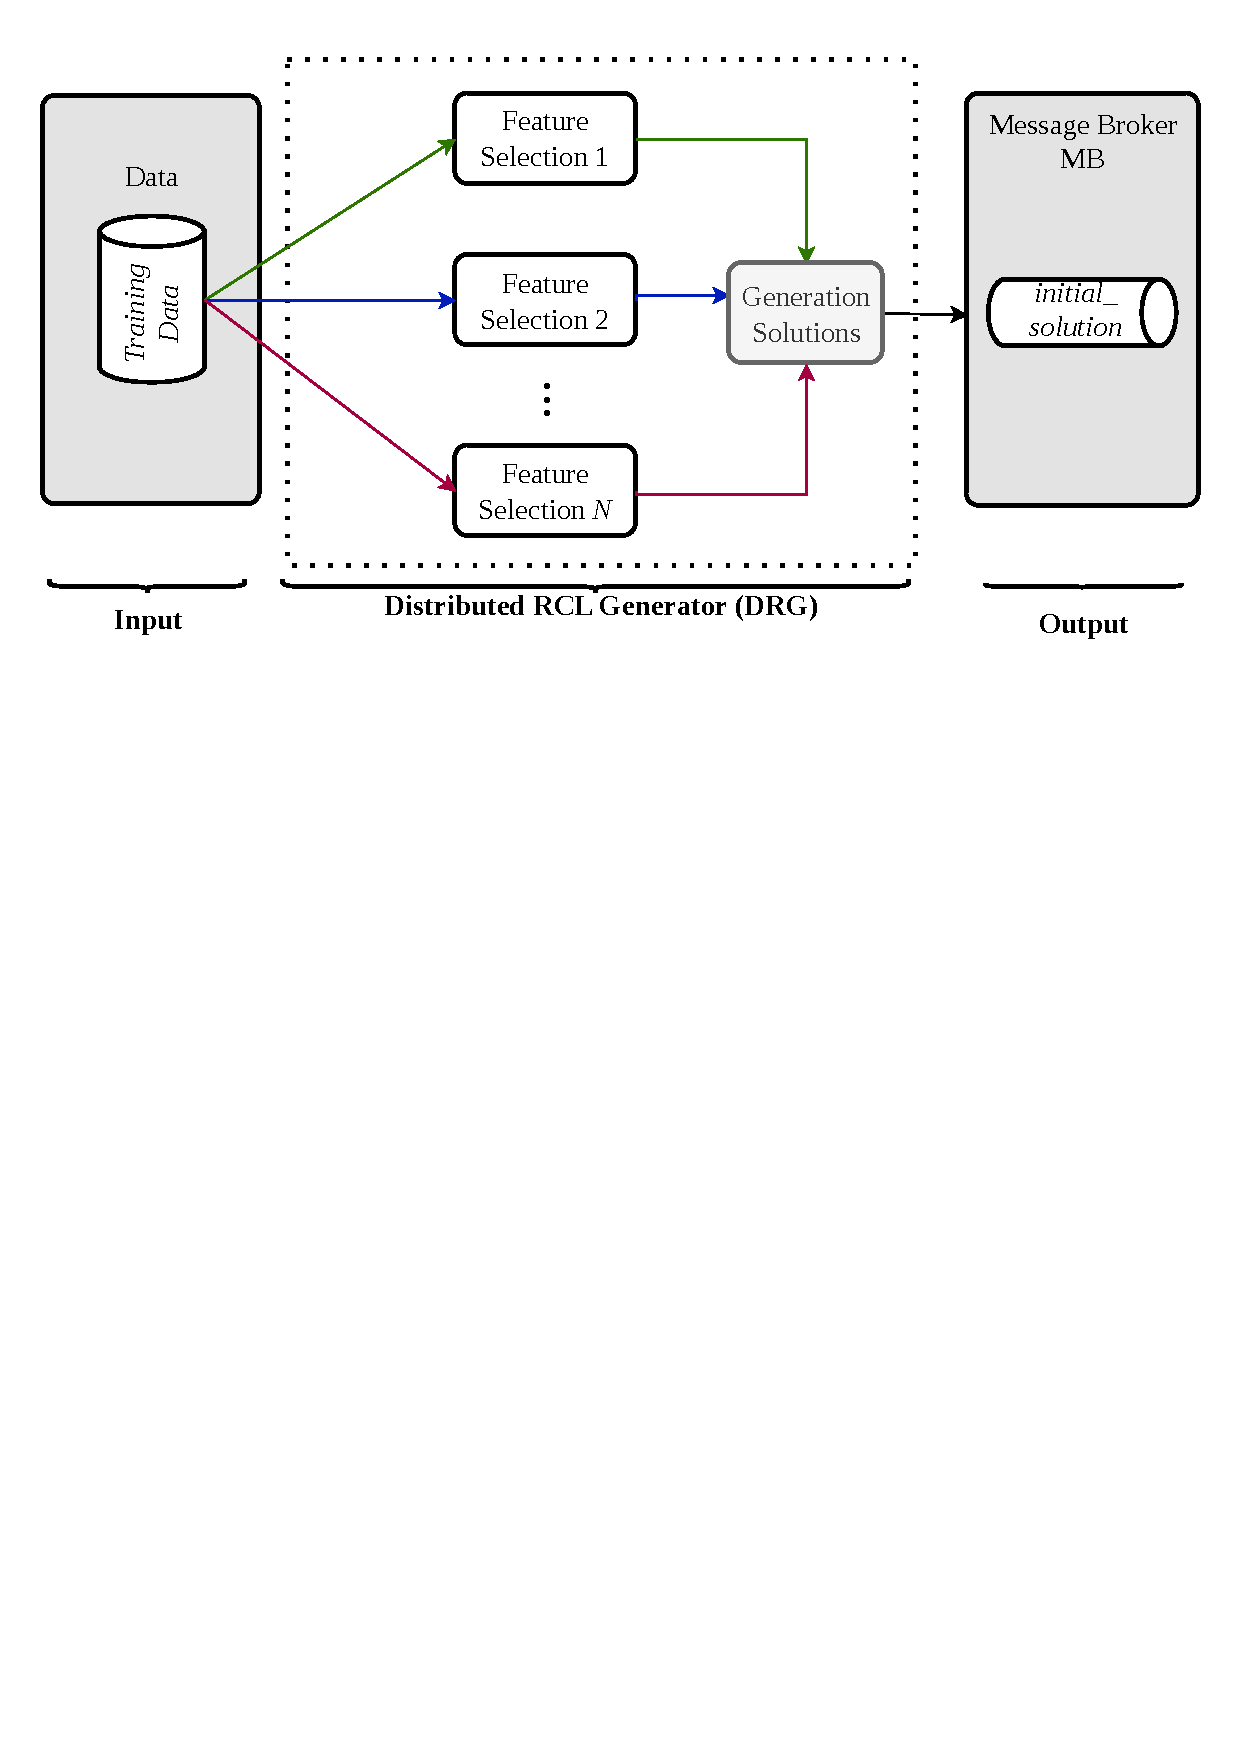
\includegraphics[width=.92\linewidth]{fig/gfshield/arquitetura-drg-generic.pdf}
  \caption{Generic DRG view with abstract data input.}
  \label{fig:app-drg-generic}
\end{figure}

\begin{figure}[!htb]
  \centering
  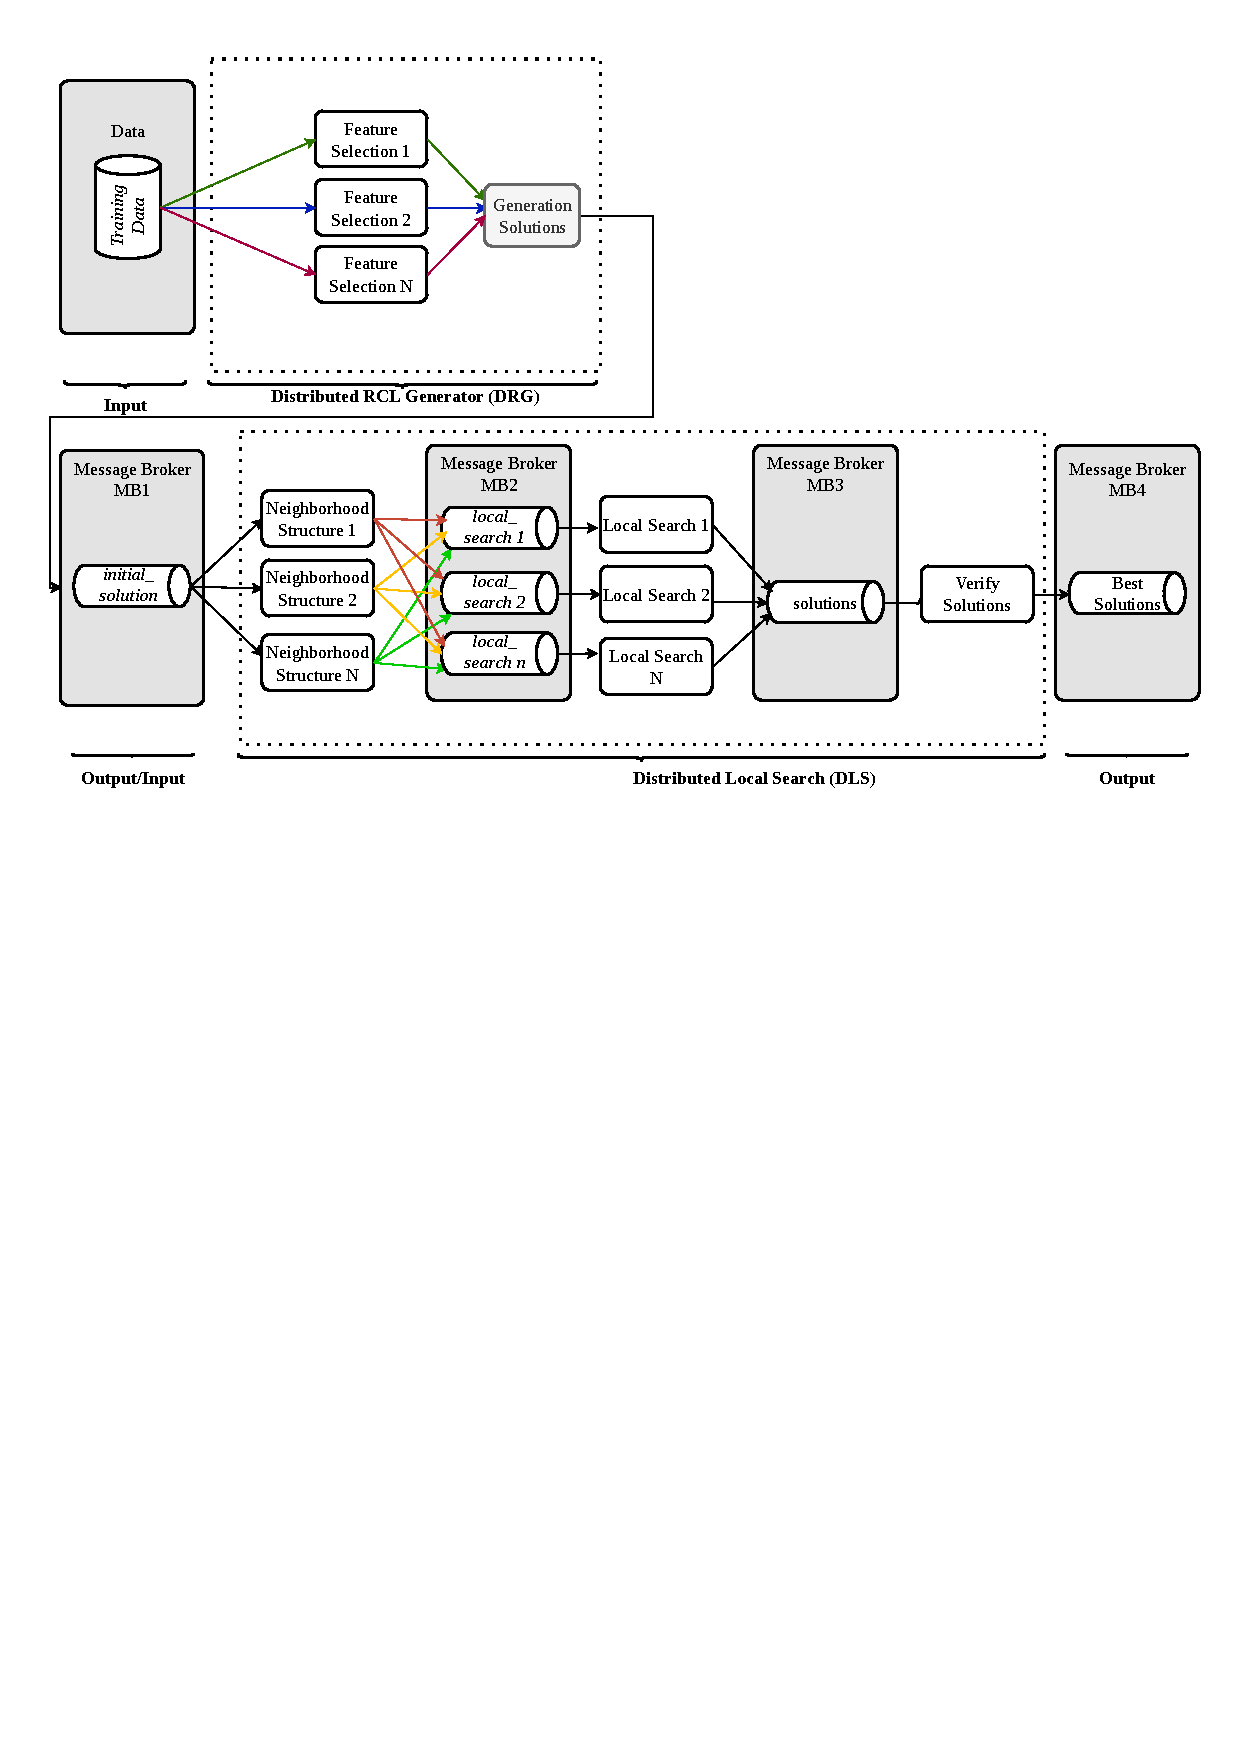
\includegraphics[width=.92\linewidth]{fig/gfshield/arquitetura-full-summary.pdf}
  \caption{Complete architecture summary.}
  \label{fig:app-architecture-summary}
\end{figure}

\end{apendicesenv}
